\section{Scope and recorded coverage}
Board PM12-\allowbreak{}K7-\allowbreak{}3A17A1\allowbreak{}B40221\allowbreak{}2223. Campaign 5ef2e2\allowbreak{}b4-\allowbreak{}c04a-\allowbreak{}4fad-\allowbreak{}b86f-\allowbreak{}a23be6\allowbreak{}21d7a7\allowbreak{}.

Recorded status: INCOMP\allowbreak{}LETE. Missing tests are NOT MEASURED. Complete selected-protocol coverage is not a calibrated whole-board release.

\begingroup\setlength{\tabcolsep}{3pt}\begin{longtable}{>{\raggedright\arraybackslash}p{0.1075\linewidth}>{\raggedright\arraybackslash}p{0.1075\linewidth}>{\raggedright\arraybackslash}p{0.1075\linewidth}>{\raggedright\arraybackslash}p{0.1075\linewidth}>{\raggedright\arraybackslash}p{0.1075\linewidth}>{\raggedright\arraybackslash}p{0.1075\linewidth}>{\raggedright\arraybackslash}p{0.1075\linewidth}>{\raggedright\arraybackslash}p{0.1075\linewidth}}\toprule
Channe\allowbreak{}l & cfd-\allowbreak{}monito\allowbreak{}r & cfd-\allowbreak{}dacs & gate-\allowbreak{}phase & tdc & adc-\allowbreak{}dc & adc-\allowbreak{}lines & integr\allowbreak{}ator\\\midrule\endhead
1 & NM & NM & NM & NM & NM & NM & NM\\
2 & NM & NM & NM & NM & NM & NM & NM\\
3 & NM & NM & NM & NM & NM & NM & NM\\
4 & NM & NM & NM & NM & NM & NM & NM\\
5 & NM & NM & NM & NM & NM & NM & NM\\
6 & NM & NM & NM & NM & NM & NM & NM\\
7 & NM & NM & NM & NM & NM & NM & NM\\
8 & NM & NM & NM & NM & NM & NM & NM\\
9 & NM & PASS & PASS & PASS & NM & NM & NM\\
10 & NM & PASS & PASS & PASS & PASS & PASS & PASS\\
11 & NM & PASS & PASS & PASS & PASS & PASS & PASS\\
12 & NM & PASS & PASS & PASS & PASS & PASS & PASS\\
\bottomrule\end{longtable}\endgroup
NM = not measured; INC = incomplete; ERR = acquisition error. No missing series is invented.
\subsection{Board-level tests}
\begingroup\setlength{\tabcolsep}{3pt}\begin{longtable}{>{\raggedright\arraybackslash}p{0.4300\linewidth}>{\raggedright\arraybackslash}p{0.4300\linewidth}}\toprule
Test & Status\allowbreak{}\\\midrule\endhead
Bounda\allowbreak{}ry scan and CPLD–FPGA connec\allowbreak{}tions & NOT\_\allowbreak{}MEASUR\allowbreak{}ED\\
MCU,\allowbreak{} CPU–FPGA commun\allowbreak{}icatio\allowbreak{}n and periph\allowbreak{}eral IDs & NOT\_\allowbreak{}MEASUR\allowbreak{}ED\\
I2C sensor\allowbreak{}s,\allowbreak{} curren\allowbreak{}ts and voltag\allowbreak{}es & NOT\_\allowbreak{}MEASUR\allowbreak{}ED\\
HDMI digita\allowbreak{}l link & NOT\_\allowbreak{}MEASUR\allowbreak{}ED\\
Ethern\allowbreak{}et/\allowbreak{}bridge\allowbreak{} diagno\allowbreak{}stic & NOT\_\allowbreak{}MEASUR\allowbreak{}ED\\
\bottomrule\end{longtable}\endgroup
\section{Fitted batches and fixture provenance}
\begingroup\setlength{\tabcolsep}{3pt}\begin{longtable}{>{\raggedright\arraybackslash}p{0.1720\linewidth}>{\raggedright\arraybackslash}p{0.1720\linewidth}>{\raggedright\arraybackslash}p{0.1720\linewidth}>{\raggedright\arraybackslash}p{0.1720\linewidth}>{\raggedright\arraybackslash}p{0.1720\linewidth}}\toprule
Batch attemp\allowbreak{}t & PM channe\allowbreak{}l & CFD label & Declar\allowbreak{}ed connec\allowbreak{}tion & Fittin\allowbreak{}g\\\midrule\endhead
ch09-\allowbreak{}12-\allowbreak{}attemp\allowbreak{}t001 & 12 & CFD01 & slot 7,\allowbreak{} RJ45 0 & Identi\allowbreak{}ty/\allowbreak{}fittin\allowbreak{}g confir\allowbreak{}med\\
ch09-\allowbreak{}12-\allowbreak{}attemp\allowbreak{}t001 & 11 & CFD02 & slot 7,\allowbreak{} RJ45 1 & Identi\allowbreak{}ty/\allowbreak{}fittin\allowbreak{}g confir\allowbreak{}med\\
ch09-\allowbreak{}12-\allowbreak{}attemp\allowbreak{}t001 & 10 & CFD03 & slot 7,\allowbreak{} RJ45 2 & Identi\allowbreak{}ty/\allowbreak{}fittin\allowbreak{}g confir\allowbreak{}med\\
ch09-\allowbreak{}12-\allowbreak{}attemp\allowbreak{}t001 & 9 & CFD04 & slot 7,\allowbreak{} RJ45 3 & Identi\allowbreak{}ty/\allowbreak{}fittin\allowbreak{}g confir\allowbreak{}med\\
\bottomrule\end{longtable}\endgroup
Fixture labels CFD01--CFD04 are provisional bench labels. Factory identities and photos remain unknown until supplied; a label is not proof of module identity. Declared cable routes must be checked physically.

Raw inputs and selected result IDs are retained in inputs/. Repeated measurements are never silently substituted.
\section{Retained attempts and explicit selection}
\begingroup\setlength{\tabcolsep}{3pt}\begin{longtable}{>{\raggedright\arraybackslash}p{0.1433\linewidth}>{\raggedright\arraybackslash}p{0.1433\linewidth}>{\raggedright\arraybackslash}p{0.1433\linewidth}>{\raggedright\arraybackslash}p{0.1433\linewidth}>{\raggedright\arraybackslash}p{0.1433\linewidth}>{\raggedright\arraybackslash}p{0.1433\linewidth}}\toprule
Result\allowbreak{} ID prefix\allowbreak{} & Test & Channe\allowbreak{}l & Fittin\allowbreak{}g & Status\allowbreak{} & Select\allowbreak{}ed\\\midrule\endhead
result\allowbreak{}-\allowbreak{}b91262\allowbreak{}35 & adc-\allowbreak{}dc & 12 & ch09-\allowbreak{}12-\allowbreak{}attemp\allowbreak{}t001 & PASS & yes\\
result\allowbreak{}-\allowbreak{}ee0613\allowbreak{}ea & adc-\allowbreak{}lines & 12 & ch09-\allowbreak{}12-\allowbreak{}attemp\allowbreak{}t001 & PASS & yes\\
result\allowbreak{}-\allowbreak{}217f5c\allowbreak{}b4 & integr\allowbreak{}ator & 12 & ch09-\allowbreak{}12-\allowbreak{}attemp\allowbreak{}t001 & PASS & yes\\
result\allowbreak{}-\allowbreak{}b99efe\allowbreak{}3a & cfd-\allowbreak{}dacs & 9 & ch09-\allowbreak{}12-\allowbreak{}attemp\allowbreak{}t001 & INCOMP\allowbreak{}LETE & no\\
result\allowbreak{}-\allowbreak{}ef5049\allowbreak{}3e & cfd-\allowbreak{}dacs & 10 & ch09-\allowbreak{}12-\allowbreak{}attemp\allowbreak{}t001 & INCOMP\allowbreak{}LETE & no\\
result\allowbreak{}-\allowbreak{}c4800a\allowbreak{}66 & cfd-\allowbreak{}dacs & 11 & ch09-\allowbreak{}12-\allowbreak{}attemp\allowbreak{}t001 & INCOMP\allowbreak{}LETE & no\\
result\allowbreak{}-\allowbreak{}c80f3b\allowbreak{}9e & cfd-\allowbreak{}dacs & 12 & ch09-\allowbreak{}12-\allowbreak{}attemp\allowbreak{}t001 & INCOMP\allowbreak{}LETE & no\\
result\allowbreak{}-\allowbreak{}9e64b4\allowbreak{}3e & cfd-\allowbreak{}dacs & 9 & ch09-\allowbreak{}12-\allowbreak{}attemp\allowbreak{}t001 & PASS & yes\\
result\allowbreak{}-\allowbreak{}0fcaad\allowbreak{}d7 & cfd-\allowbreak{}dacs & 10 & ch09-\allowbreak{}12-\allowbreak{}attemp\allowbreak{}t001 & PASS & yes\\
result\allowbreak{}-\allowbreak{}8b6b8a\allowbreak{}a7 & cfd-\allowbreak{}dacs & 11 & ch09-\allowbreak{}12-\allowbreak{}attemp\allowbreak{}t001 & PASS & yes\\
result\allowbreak{}-\allowbreak{}b4c6c4\allowbreak{}97 & cfd-\allowbreak{}dacs & 12 & ch09-\allowbreak{}12-\allowbreak{}attemp\allowbreak{}t001 & PASS & yes\\
result\allowbreak{}-\allowbreak{}aa2f2b\allowbreak{}7c & adc-\allowbreak{}dc & 11 & ch09-\allowbreak{}12-\allowbreak{}attemp\allowbreak{}t001 & PASS & yes\\
result\allowbreak{}-\allowbreak{}fa68f8\allowbreak{}09 & adc-\allowbreak{}lines & 11 & ch09-\allowbreak{}12-\allowbreak{}attemp\allowbreak{}t001 & PASS & yes\\
result\allowbreak{}-\allowbreak{}021f9e\allowbreak{}97 & integr\allowbreak{}ator & 11 & ch09-\allowbreak{}12-\allowbreak{}attemp\allowbreak{}t001 & PASS & yes\\
result\allowbreak{}-\allowbreak{}317b8d\allowbreak{}60 & adc-\allowbreak{}dc & 10 & ch09-\allowbreak{}12-\allowbreak{}attemp\allowbreak{}t001 & PASS & yes\\
result\allowbreak{}-\allowbreak{}0386d7\allowbreak{}66 & adc-\allowbreak{}lines & 10 & ch09-\allowbreak{}12-\allowbreak{}attemp\allowbreak{}t001 & PASS & yes\\
result\allowbreak{}-\allowbreak{}e87c1c\allowbreak{}5e & integr\allowbreak{}ator & 10 & ch09-\allowbreak{}12-\allowbreak{}attemp\allowbreak{}t001 & PASS & yes\\
result\allowbreak{}-\allowbreak{}164215\allowbreak{}3e & tdc & 12 & ch09-\allowbreak{}12-\allowbreak{}attemp\allowbreak{}t001 & PASS & yes\\
result\allowbreak{}-\allowbreak{}5f833b\allowbreak{}a0 & tdc & 11 & ch09-\allowbreak{}12-\allowbreak{}attemp\allowbreak{}t001 & PASS & yes\\
result\allowbreak{}-\allowbreak{}cdf234\allowbreak{}1e & tdc & 10 & ch09-\allowbreak{}12-\allowbreak{}attemp\allowbreak{}t001 & PASS & yes\\
result\allowbreak{}-\allowbreak{}5e3a4c\allowbreak{}64 & tdc & 9 & ch09-\allowbreak{}12-\allowbreak{}attemp\allowbreak{}t001 & PASS & yes\\
result\allowbreak{}-\allowbreak{}d2e5cd\allowbreak{}6c & gate-\allowbreak{}phase & 12 & ch09-\allowbreak{}12-\allowbreak{}attemp\allowbreak{}t001 & PASS & yes\\
result\allowbreak{}-\allowbreak{}769a57\allowbreak{}17 & gate-\allowbreak{}phase & 11 & ch09-\allowbreak{}12-\allowbreak{}attemp\allowbreak{}t001 & PASS & yes\\
result\allowbreak{}-\allowbreak{}5b389a\allowbreak{}db & gate-\allowbreak{}phase & 10 & ch09-\allowbreak{}12-\allowbreak{}attemp\allowbreak{}t001 & PASS & yes\\
result\allowbreak{}-\allowbreak{}a00721\allowbreak{}bb & gate-\allowbreak{}phase & 9 & ch09-\allowbreak{}12-\allowbreak{}attemp\allowbreak{}t001 & PASS & yes\\
\bottomrule\end{longtable}\endgroup
All attempts, including failures and rejected repeats, remain in the archived inputs. The coverage matrix uses only the explicitly selected attempt.
\section{Selected measurement conditions and limits}
\begingroup\setlength{\tabcolsep}{3pt}\begin{longtable}{>{\raggedright\arraybackslash}p{0.2867\linewidth}>{\raggedright\arraybackslash}p{0.2867\linewidth}>{\raggedright\arraybackslash}p{0.2867\linewidth}}\toprule
Test & Physic\allowbreak{}al channe\allowbreak{}l & Confir\allowbreak{}med stimul\allowbreak{}us connec\allowbreak{}tion\\\midrule\endhead
adc-\allowbreak{}dc & 12 & \{"dac\_\allowbreak{}channe\allowbreak{}ls": [0,\allowbreak{} 1],\allowbreak{} "stimul\allowbreak{}us\_\allowbreak{}channe\allowbreak{}l": 12,\allowbreak{} "usb\_\allowbreak{}input": "J8"\}\\
adc-\allowbreak{}lines & 12 & \{"dac\_\allowbreak{}channe\allowbreak{}ls": [0,\allowbreak{} 1],\allowbreak{} "stimul\allowbreak{}us\_\allowbreak{}channe\allowbreak{}l": 12,\allowbreak{} "usb\_\allowbreak{}input": "J8"\}\\
integr\allowbreak{}ator & 12 & \{"dac\_\allowbreak{}channe\allowbreak{}ls": [2,\allowbreak{} 3],\allowbreak{} "stimul\allowbreak{}us\_\allowbreak{}channe\allowbreak{}l": 12,\allowbreak{} "usb\_\allowbreak{}input": "J6"\}\\
cfd-\allowbreak{}dacs & 9 & \{"select\allowbreak{}ion": "one monito\allowbreak{}r mux enable\allowbreak{}d; all others\allowbreak{} inhibi\allowbreak{}ted",\allowbreak{} "shared\allowbreak{}\_\allowbreak{}monito\allowbreak{}r\_\allowbreak{}channe\allowbreak{}ls": [9,\allowbreak{} 10,\allowbreak{} 11,\allowbreak{} 12]\}\\
cfd-\allowbreak{}dacs & 10 & \{"select\allowbreak{}ion": "one monito\allowbreak{}r mux enable\allowbreak{}d; all others\allowbreak{} inhibi\allowbreak{}ted",\allowbreak{} "shared\allowbreak{}\_\allowbreak{}monito\allowbreak{}r\_\allowbreak{}channe\allowbreak{}ls": [9,\allowbreak{} 10,\allowbreak{} 11,\allowbreak{} 12]\}\\
cfd-\allowbreak{}dacs & 11 & \{"select\allowbreak{}ion": "one monito\allowbreak{}r mux enable\allowbreak{}d; all others\allowbreak{} inhibi\allowbreak{}ted",\allowbreak{} "shared\allowbreak{}\_\allowbreak{}monito\allowbreak{}r\_\allowbreak{}channe\allowbreak{}ls": [9,\allowbreak{} 10,\allowbreak{} 11,\allowbreak{} 12]\}\\
cfd-\allowbreak{}dacs & 12 & \{"select\allowbreak{}ion": "one monito\allowbreak{}r mux enable\allowbreak{}d; all others\allowbreak{} inhibi\allowbreak{}ted",\allowbreak{} "shared\allowbreak{}\_\allowbreak{}monito\allowbreak{}r\_\allowbreak{}channe\allowbreak{}ls": [9,\allowbreak{} 10,\allowbreak{} 11,\allowbreak{} 12]\}\\
adc-\allowbreak{}dc & 11 & \{"dac\_\allowbreak{}channe\allowbreak{}ls": [0,\allowbreak{} 1],\allowbreak{} "stimul\allowbreak{}us\_\allowbreak{}channe\allowbreak{}l": 11,\allowbreak{} "usb\_\allowbreak{}input": "J8"\}\\
adc-\allowbreak{}lines & 11 & \{"dac\_\allowbreak{}channe\allowbreak{}ls": [0,\allowbreak{} 1],\allowbreak{} "stimul\allowbreak{}us\_\allowbreak{}channe\allowbreak{}l": 11,\allowbreak{} "usb\_\allowbreak{}input": "J8"\}\\
integr\allowbreak{}ator & 11 & \{"dac\_\allowbreak{}channe\allowbreak{}ls": [2,\allowbreak{} 3],\allowbreak{} "stimul\allowbreak{}us\_\allowbreak{}channe\allowbreak{}l": 11,\allowbreak{} "usb\_\allowbreak{}input": "J6"\}\\
adc-\allowbreak{}dc & 10 & \{"dac\_\allowbreak{}channe\allowbreak{}ls": [0,\allowbreak{} 1],\allowbreak{} "stimul\allowbreak{}us\_\allowbreak{}channe\allowbreak{}l": 10,\allowbreak{} "usb\_\allowbreak{}input": "J8"\}\\
adc-\allowbreak{}lines & 10 & \{"dac\_\allowbreak{}channe\allowbreak{}ls": [0,\allowbreak{} 1],\allowbreak{} "stimul\allowbreak{}us\_\allowbreak{}channe\allowbreak{}l": 10,\allowbreak{} "usb\_\allowbreak{}input": "J8"\}\\
integr\allowbreak{}ator & 10 & \{"dac\_\allowbreak{}channe\allowbreak{}ls": [2,\allowbreak{} 3],\allowbreak{} "stimul\allowbreak{}us\_\allowbreak{}channe\allowbreak{}l": 10,\allowbreak{} "usb\_\allowbreak{}input": "J6"\}\\
tdc & 12 & \{"phase\_\allowbreak{}lanes": [8,\allowbreak{} 9],\allowbreak{} "rj45\_\allowbreak{}port": 0,\allowbreak{} "slot": 7,\allowbreak{} "stimul\allowbreak{}us\_\allowbreak{}dio": 0\}\\
tdc & 11 & \{"phase\_\allowbreak{}lanes": [10,\allowbreak{} 11],\allowbreak{} "rj45\_\allowbreak{}port": 1,\allowbreak{} "slot": 7,\allowbreak{} "stimul\allowbreak{}us\_\allowbreak{}dio": 4\}\\
tdc & 10 & \{"phase\_\allowbreak{}lanes": [12,\allowbreak{} 13],\allowbreak{} "rj45\_\allowbreak{}port": 2,\allowbreak{} "slot": 7,\allowbreak{} "stimul\allowbreak{}us\_\allowbreak{}dio": 8\}\\
tdc & 9 & \{"phase\_\allowbreak{}lanes": [14,\allowbreak{} 15],\allowbreak{} "rj45\_\allowbreak{}port": 3,\allowbreak{} "slot": 7,\allowbreak{} "stimul\allowbreak{}us\_\allowbreak{}dio": 12\}\\
gate-\allowbreak{}phase & 12 & \{"phase\_\allowbreak{}lanes": [8,\allowbreak{} 9],\allowbreak{} "rj45\_\allowbreak{}port": 0,\allowbreak{} "slot": 7,\allowbreak{} "stimul\allowbreak{}us\_\allowbreak{}dio": 0\}\\
gate-\allowbreak{}phase & 11 & \{"phase\_\allowbreak{}lanes": [10,\allowbreak{} 11],\allowbreak{} "rj45\_\allowbreak{}port": 1,\allowbreak{} "slot": 7,\allowbreak{} "stimul\allowbreak{}us\_\allowbreak{}dio": 4\}\\
gate-\allowbreak{}phase & 10 & \{"phase\_\allowbreak{}lanes": [12,\allowbreak{} 13],\allowbreak{} "rj45\_\allowbreak{}port": 2,\allowbreak{} "slot": 7,\allowbreak{} "stimul\allowbreak{}us\_\allowbreak{}dio": 8\}\\
gate-\allowbreak{}phase & 9 & \{"phase\_\allowbreak{}lanes": [14,\allowbreak{} 15],\allowbreak{} "rj45\_\allowbreak{}port": 3,\allowbreak{} "slot": 7,\allowbreak{} "stimul\allowbreak{}us\_\allowbreak{}dio": 12\}\\
\bottomrule\end{longtable}\endgroup
\subsection{Common hardware configuration}
\begingroup\setlength{\tabcolsep}{3pt}\begin{longtable}{>{\raggedright\arraybackslash}p{0.4300\linewidth}>{\raggedright\arraybackslash}p{0.4300\linewidth}}\toprule
Settin\allowbreak{}g & Record\allowbreak{}ed value\\\midrule\endhead
clock\_\allowbreak{}profil\allowbreak{}e.adc\_\allowbreak{}rate & 2x refere\allowbreak{}nce\\
clock\_\allowbreak{}profil\allowbreak{}e.kasli\_\allowbreak{}rate & 3x refere\allowbreak{}nce\\
clock\_\allowbreak{}profil\allowbreak{}e.refere\allowbreak{}nce\_\allowbreak{}mhz & 40.0787\\
cpld\_\allowbreak{}gate\_\allowbreak{}mode & origin\allowbreak{}al INTA/\allowbreak{}INTB enable\allowbreak{}d,\allowbreak{} nomina\allowbreak{}l20MHz\allowbreak{}\\
kasli\_\allowbreak{}build.ABI & CFD4\\
kasli\_\allowbreak{}build.expect\allowbreak{}ed\_\allowbreak{}bit\_\allowbreak{}sha256\allowbreak{} & a71a08\allowbreak{}a25862\allowbreak{}0b0e5a\allowbreak{}52c5d0\allowbreak{}3aefd8\allowbreak{}c69040\allowbreak{}c9d15e\allowbreak{}8de639\allowbreak{}1c484a\allowbreak{}c182b7\allowbreak{}173b\\
pm\_\allowbreak{}build & c7c42d\allowbreak{}28\\
\bottomrule\end{longtable}\endgroup
\subsection{adc-\allowbreak{}dc}
\begingroup\setlength{\tabcolsep}{3pt}\begin{longtable}{>{\raggedright\arraybackslash}p{0.4300\linewidth}>{\raggedright\arraybackslash}p{0.4300\linewidth}}\toprule
Settin\allowbreak{}g & Record\allowbreak{}ed value\\\midrule\endhead
method\allowbreak{} & "direct\allowbreak{}-\allowbreak{}ADC-\allowbreak{}DC-\allowbreak{}v1"\\
stimul\allowbreak{}us\_\allowbreak{}points\allowbreak{}\_\allowbreak{}per\_\allowbreak{}bank & 257\\
comman\allowbreak{}ded\_\allowbreak{}range\_\allowbreak{}V & [-\allowbreak{}1.2,\allowbreak{} 1.2]\\
common\allowbreak{}\_\allowbreak{}mode\_\allowbreak{}V & 1.0\\
dac\_\allowbreak{}channe\allowbreak{}ls & [0,\allowbreak{} 1]\\
fit\_\allowbreak{}interv\allowbreak{}al\_\allowbreak{}V & [-\allowbreak{}0.8,\allowbreak{} 0.8]\\
fft\_\allowbreak{}sample\allowbreak{}\_\allowbreak{}rate\_\allowbreak{}assume\allowbreak{}d\_\allowbreak{}Hz & 801574\allowbreak{}00\\
integr\allowbreak{}ator\_\allowbreak{}input\_\allowbreak{}parked\allowbreak{}\_\allowbreak{}V & [2.048000\allowbreak{}1,\allowbreak{} 1.024000\allowbreak{}05]\\
\bottomrule\end{longtable}\endgroup
\subsection{adc-\allowbreak{}lines}
\begingroup\setlength{\tabcolsep}{3pt}\begin{longtable}{>{\raggedright\arraybackslash}p{0.4300\linewidth}>{\raggedright\arraybackslash}p{0.4300\linewidth}}\toprule
Settin\allowbreak{}g & Record\allowbreak{}ed value\\\midrule\endhead
method\allowbreak{} & "adjace\allowbreak{}nt-\allowbreak{}pair-\allowbreak{}states\allowbreak{}-\allowbreak{}v1"\\
stimul\allowbreak{}us\_\allowbreak{}points\allowbreak{}\_\allowbreak{}per\_\allowbreak{}bank & 257\\
comman\allowbreak{}ded\_\allowbreak{}range\_\allowbreak{}V & [-\allowbreak{}1.2,\allowbreak{} 1.2]\\
common\allowbreak{}\_\allowbreak{}mode\_\allowbreak{}V & 1.0\\
dac\_\allowbreak{}channe\allowbreak{}ls & [0,\allowbreak{} 1]\\
fit\_\allowbreak{}interv\allowbreak{}al\_\allowbreak{}V & [-\allowbreak{}0.8,\allowbreak{} 0.8]\\
fft\_\allowbreak{}sample\allowbreak{}\_\allowbreak{}rate\_\allowbreak{}assume\allowbreak{}d\_\allowbreak{}Hz & 801574\allowbreak{}00\\
integr\allowbreak{}ator\_\allowbreak{}input\_\allowbreak{}parked\allowbreak{}\_\allowbreak{}V & [2.048000\allowbreak{}1,\allowbreak{} 1.024000\allowbreak{}05]\\
\bottomrule\end{longtable}\endgroup
\subsection{cfd-\allowbreak{}dacs}
\begingroup\setlength{\tabcolsep}{3pt}\begin{longtable}{>{\raggedright\arraybackslash}p{0.4300\linewidth}>{\raggedright\arraybackslash}p{0.4300\linewidth}}\toprule
Settin\allowbreak{}g & Record\allowbreak{}ed value\\\midrule\endhead
method\allowbreak{} & "shared\allowbreak{}-\allowbreak{}monito\allowbreak{}r-\allowbreak{}SMU-\allowbreak{}BCD-\allowbreak{}v1"\\
instru\allowbreak{}ment\_\allowbreak{}identi\allowbreak{}ty & "Keysig\allowbreak{}ht Techno\allowbreak{}logies\allowbreak{},\allowbreak{}B2910B\allowbreak{}L,\allowbreak{}MY6332\allowbreak{}0299,\allowbreak{}5.0.2429.8966"\\
sense & "Force HI/\allowbreak{}LO,\allowbreak{} local"\\
source\allowbreak{}\_\allowbreak{}curren\allowbreak{}t\_\allowbreak{}A & 0\\
source\allowbreak{}\_\allowbreak{}range\_\allowbreak{}A & 1e-\allowbreak{}06\\
voltag\allowbreak{}e\_\allowbreak{}range\_\allowbreak{}V & 20\\
nplc & 1\\
settli\allowbreak{}ng\_\allowbreak{}s & 0.1\\
points\allowbreak{} & 101\\
repeat\allowbreak{}s & 3\\
limits\allowbreak{} & \{"repeat\allowbreak{}\_\allowbreak{}std\_\allowbreak{}V": 0.001,\allowbreak{} "revers\allowbreak{}e\_\allowbreak{}step\_\allowbreak{}V": 0.0002,\allowbreak{} "span\_\allowbreak{}relati\allowbreak{}ve\_\allowbreak{}error": 0.05\}\\
post\_\allowbreak{}scan\_\allowbreak{}verifi\allowbreak{}cation\allowbreak{} & "SMU OFF/\allowbreak{}HIZ,\allowbreak{} four monito\allowbreak{}r muxes inhibi\allowbreak{}ted,\allowbreak{} explic\allowbreak{}it TCA masks0\allowbreak{}"\\
\bottomrule\end{longtable}\endgroup
\subsection{gate-\allowbreak{}phase}
\begingroup\setlength{\tabcolsep}{3pt}\begin{longtable}{>{\raggedright\arraybackslash}p{0.4300\linewidth}>{\raggedright\arraybackslash}p{0.4300\linewidth}}\toprule
Settin\allowbreak{}g & Record\allowbreak{}ed value\\\midrule\endhead
method\allowbreak{} & "DAC-\allowbreak{}A-\allowbreak{}ISERDE\allowbreak{}S-\allowbreak{}gate-\allowbreak{}phase-\allowbreak{}v1"\\
codes & [0,\allowbreak{} 655,\allowbreak{} 1311,\allowbreak{} 1966,\allowbreak{} 2621,\allowbreak{} 3277,\allowbreak{} 3932,\allowbreak{} 4587,\allowbreak{} 5243,\allowbreak{} 5898,\allowbreak{} 6554,\allowbreak{} 7209,\allowbreak{} 7864,\allowbreak{} 8520,\allowbreak{} 9175,\allowbreak{} 9830,\allowbreak{} 10486,\allowbreak{} 11141,\allowbreak{} 11796,\allowbreak{} 12452,\allowbreak{} 13107,\allowbreak{} 13762,\allowbreak{} 14418,\allowbreak{} 15073,\allowbreak{} 15728,\allowbreak{} 16384,\allowbreak{} 17039,\allowbreak{} 17694,\allowbreak{} 18350,\allowbreak{} 19005,\allowbreak{} 19661,\allowbreak{} 20316,\allowbreak{} 20971,\allowbreak{} 21627,\allowbreak{} 22282,\allowbreak{} 22937,\allowbreak{} 23593,\allowbreak{} 24248,\allowbreak{} 24903,\allowbreak{} 25559,\allowbreak{} 26214,\allowbreak{} 26869,\allowbreak{} 27525,\allowbreak{} 28180,\allowbreak{} 28835,\allowbreak{} 29491,\allowbreak{} 30146,\allowbreak{} 30801,\allowbreak{} 31457,\allowbreak{} 32112,\allowbreak{} 32768,\allowbreak{} 33423,\allowbreak{} 34078,\allowbreak{} 34734,\allowbreak{} 35389,\allowbreak{} 36044,\allowbreak{} 36700,\allowbreak{} 37355,\allowbreak{} 38010,\allowbreak{} 38666,\allowbreak{} 39321,\allowbreak{} 39976,\allowbreak{} 40632,\allowbreak{} 41287,\allowbreak{} 41942,\allowbreak{} 42598,\allowbreak{} 43253,\allowbreak{} 43908,\allowbreak{} 44564,\allowbreak{} 45219,\allowbreak{} 45875,\allowbreak{} 46530,\allowbreak{} 47185,\allowbreak{} 47841,\allowbreak{} 48496,\allowbreak{} 49151,\allowbreak{} 49807,\allowbreak{} 50462,\allowbreak{} 51117,\allowbreak{} 51773,\allowbreak{} 52428,\allowbreak{} 53083,\allowbreak{} 53739,\allowbreak{} 54394,\allowbreak{} 55049,\allowbreak{} 55705,\allowbreak{} 56360,\allowbreak{} 57015,\allowbreak{} 57671,\allowbreak{} 58326,\allowbreak{} 58982,\allowbreak{} 59637,\allowbreak{} 60292,\allowbreak{} 60948,\allowbreak{} 61603,\allowbreak{} 62258,\allowbreak{} 62914,\allowbreak{} 63569,\allowbreak{} 64224,\allowbreak{} 64880,\allowbreak{} 65535]\\
sample\allowbreak{}\_\allowbreak{}hz & 961888\allowbreak{}800.0\\
gate\_\allowbreak{}period\allowbreak{}\_\allowbreak{}bins & 48\\
captur\allowbreak{}e\_\allowbreak{}words & 4095\\
minimu\allowbreak{}m\_\allowbreak{}functi\allowbreak{}onal\_\allowbreak{}excurs\allowbreak{}ion\_\allowbreak{}ns & 5\\
\bottomrule\end{longtable}\endgroup
\subsection{integr\allowbreak{}ator}
\begingroup\setlength{\tabcolsep}{3pt}\begin{longtable}{>{\raggedright\arraybackslash}p{0.4300\linewidth}>{\raggedright\arraybackslash}p{0.4300\linewidth}}\toprule
Settin\allowbreak{}g & Record\allowbreak{}ed value\\\midrule\endhead
method\allowbreak{} & "signed\allowbreak{}-\allowbreak{}integr\allowbreak{}ation-\allowbreak{}pair-\allowbreak{}v1"\\
dac\_\allowbreak{}channe\allowbreak{}ls & [2,\allowbreak{} 3]\\
base\_\allowbreak{}V & [1.024,\allowbreak{} 2.048]\\
coarse\allowbreak{}\_\allowbreak{}offset\allowbreak{}s\_\allowbreak{}V & [-\allowbreak{}0.099999\allowbreak{}999999\allowbreak{}99987,\allowbreak{} -\allowbreak{}0.080000\allowbreak{}000000\allowbreak{}00007,\allowbreak{} -\allowbreak{}0.059999\allowbreak{}999999\allowbreak{}99983,\allowbreak{} -\allowbreak{}0.040000\allowbreak{}000000\allowbreak{}000036\allowbreak{},\allowbreak{} -\allowbreak{}0.019999\allowbreak{}999999\allowbreak{}999796\allowbreak{},\allowbreak{} -\allowbreak{}0.010000\allowbreak{}000000\allowbreak{}000009\allowbreak{},\allowbreak{} 0.0,\allowbreak{} 0.009999\allowbreak{}999999\allowbreak{}999787\allowbreak{},\allowbreak{} 0.020000\allowbreak{}000000\allowbreak{}00024,\allowbreak{} 0.040000\allowbreak{}000000\allowbreak{}000036\allowbreak{},\allowbreak{} 0.060000\allowbreak{}000000\allowbreak{}000275\allowbreak{},\allowbreak{} 0.080000\allowbreak{}000000\allowbreak{}00007,\allowbreak{} 0.100000\allowbreak{}000000\allowbreak{}00009]\\
fine\_\allowbreak{}method\allowbreak{} & "26 points\allowbreak{},\allowbreak{}0.4mV step around\allowbreak{} coarse\allowbreak{} estima\allowbreak{}te"\\
return\allowbreak{}\_\allowbreak{}method\allowbreak{} & "two candid\allowbreak{}ate revisi\allowbreak{}ts and +/\allowbreak{}-\allowbreak{}5mV offset\allowbreak{}s;near-\allowbreak{}zero <=2codes\allowbreak{}; signed\allowbreak{} respon\allowbreak{}se >4codes\allowbreak{}"\\
\bottomrule\end{longtable}\endgroup
\subsection{tdc}
\begingroup\setlength{\tabcolsep}{3pt}\begin{longtable}{>{\raggedright\arraybackslash}p{0.4300\linewidth}>{\raggedright\arraybackslash}p{0.4300\linewidth}}\toprule
Settin\allowbreak{}g & Record\allowbreak{}ed value\\\midrule\endhead
method\allowbreak{} & "finite\allowbreak{}-\allowbreak{}OSERDE\allowbreak{}S-\allowbreak{}TDC-\allowbreak{}phase-\allowbreak{}v1"\\
phase\_\allowbreak{}slots & [24,\allowbreak{} 25,\allowbreak{} 26,\allowbreak{} 27,\allowbreak{} 28,\allowbreak{} 29,\allowbreak{} 30,\allowbreak{} 31,\allowbreak{} 32,\allowbreak{} 33,\allowbreak{} 34,\allowbreak{} 35,\allowbreak{} 36,\allowbreak{} 37,\allowbreak{} 38,\allowbreak{} 39,\allowbreak{} 40,\allowbreak{} 41,\allowbreak{} 42,\allowbreak{} 43,\allowbreak{} 44,\allowbreak{} 45,\allowbreak{} 46,\allowbreak{} 47,\allowbreak{} 48]\\
sample\allowbreak{}\_\allowbreak{}hz & 961888\allowbreak{}800.0\\
events\allowbreak{}\_\allowbreak{}per\_\allowbreak{}phase & 128\\
discov\allowbreak{}ery\_\allowbreak{}events\allowbreak{} & 16\\
respon\allowbreak{}se\_\allowbreak{}slope\_\allowbreak{}window\allowbreak{} & [-\allowbreak{}60,\allowbreak{} -\allowbreak{}20]\\
maximu\allowbreak{}m\_\allowbreak{}residu\allowbreak{}al\_\allowbreak{}fine\_\allowbreak{}codes & 10\\
\bottomrule\end{longtable}\endgroup
Comman\allowbreak{}ded DAC voltag\allowbreak{}es,\allowbreak{} whole connec\allowbreak{}ted chain; not calibr\allowbreak{}ated ADC-\allowbreak{}only INL/\allowbreak{}noise or electr\allowbreak{}ical contin\allowbreak{}uity proof.

Effect\allowbreak{}ive differ\allowbreak{}ential\allowbreak{} whole-\allowbreak{}chain balanc\allowbreak{}e; wavefo\allowbreak{}rm-\allowbreak{}based integr\allowbreak{}ation pair,\allowbreak{} not an absolu\allowbreak{}te gate timest\allowbreak{}amp or calibr\allowbreak{}ated opamp bias.

Fine modulo\allowbreak{}128 unwrap\allowbreak{}ped by neares\allowbreak{}t contin\allowbreak{}uation\allowbreak{}; coarse\allowbreak{} fields\allowbreak{} retain\allowbreak{}ed withou\allowbreak{}t repair\allowbreak{}. Progra\allowbreak{}mmed slot1.0396ns\allowbreak{} assume\allowbreak{}s40.0787MH\allowbreak{}z; not calibr\allowbreak{}ated TDC timing\allowbreak{} or intrin\allowbreak{}sic jitter\allowbreak{}.

Functi\allowbreak{}onal assemb\allowbreak{}led-\allowbreak{}chain transf\allowbreak{}er check: span within\allowbreak{}5\% of schema\allowbreak{}tic scalin\allowbreak{}g,\allowbreak{} revers\allowbreak{}e step <=0.2mV,\allowbreak{} repeat\allowbreak{} standa\allowbreak{}rd deviat\allowbreak{}ion <=1mV. Not tracea\allowbreak{}ble calibr\allowbreak{}ation or exhaus\allowbreak{}tive16\allowbreak{}-\allowbreak{}bit INL/\allowbreak{}DNL. DAC-\allowbreak{}A unchan\allowbreak{}ged; exerci\allowbreak{}sed B/\allowbreak{}C/\allowbreak{}D end at0000\allowbreak{}..

Occupa\allowbreak{}ncy-\allowbreak{}weight\allowbreak{}ed sample\allowbreak{}d phase centro\allowbreak{}id; nomina\allowbreak{}l1.0396ns\allowbreak{} bins and49.9ns gate period\allowbreak{}. Neares\allowbreak{}t-\allowbreak{}contin\allowbreak{}uation\allowbreak{} unwrap\allowbreak{}; discon\allowbreak{}tinuit\allowbreak{}ies retain\allowbreak{}ed. No calibr\allowbreak{}ated sub-\allowbreak{}bin precis\allowbreak{}ion or indepe\allowbreak{}ndent-\allowbreak{}edge sqrt(N) uncert\allowbreak{}ainty. DAC A comman\allowbreak{}ded000\allowbreak{}0 at cleanu\allowbreak{}p,\allowbreak{} withou\allowbreak{}t hardwa\allowbreak{}re code readba\allowbreak{}ck.

integr\allowbreak{}ator; physic\allowbreak{}al channe\allowbreak{}l 10: The coarse\allowbreak{} wavefo\allowbreak{}rm assign\allowbreak{}ment produc\allowbreak{}es an additi\allowbreak{}onal positi\allowbreak{}ve-\allowbreak{}going sign crossi\allowbreak{}ng near +40mV. It was not accept\allowbreak{}ed as balanc\allowbreak{}e. Fine acquis\allowbreak{}ition used the centra\allowbreak{}l negati\allowbreak{}ve-\allowbreak{}going crossi\allowbreak{}ng for this revers\allowbreak{}ed input coordi\allowbreak{}nate,\allowbreak{} then confir\allowbreak{}med it with indepe\allowbreak{}ndent candid\allowbreak{}ate revisi\allowbreak{}ts and +/\allowbreak{}-\allowbreak{}5mV contro\allowbreak{}ls. The origin\allowbreak{}al coarse\allowbreak{} data and both contro\allowbreak{}ller versio\allowbreak{}ns remain\allowbreak{} archiv\allowbreak{}ed.

ADC total RMS includes the complete connected chain and periodic gate feedthrough. The four-phase-removed RMS removes the mean of each sample phase; it is a residual statistic, not an intrinsic ADC noise specification. FFT and time axes use the declared clock frequency, not an independent frequency measurement.

\section{Measurements and common channel plots}
\begingroup\setlength{\tabcolsep}{3pt}\begin{longtable}{>{\raggedright\arraybackslash}p{0.1433\linewidth}>{\raggedright\arraybackslash}p{0.1433\linewidth}>{\raggedright\arraybackslash}p{0.1433\linewidth}>{\raggedright\arraybackslash}p{0.1433\linewidth}>{\raggedright\arraybackslash}p{0.1433\linewidth}>{\raggedright\arraybackslash}p{0.1433\linewidth}}\toprule
Test & Channe\allowbreak{}l & Bank & Observ\allowbreak{}able & Value & Unit\\\midrule\endhead
adc-\allowbreak{}dc & 12 & A & gain & -\allowbreak{}1784.205440\allowbreak{}671235\allowbreak{} & code/\allowbreak{}V\\
adc-\allowbreak{}dc & 12 & A & zero\_\allowbreak{}mean & 2162.081133\allowbreak{}919843\allowbreak{}5 & code\\
adc-\allowbreak{}dc & 12 & A & zero\_\allowbreak{}total\_\allowbreak{}rms & 56.227545\allowbreak{}889877\allowbreak{}61 & code\\
adc-\allowbreak{}dc & 12 & A & zero\_\allowbreak{}four\_\allowbreak{}phase\_\allowbreak{}remove\allowbreak{}d\_\allowbreak{}rms & 0.592637\allowbreak{}125072\allowbreak{}8474 & code\\
adc-\allowbreak{}dc & 12 & B & gain & -\allowbreak{}1784.269486\allowbreak{}954563\allowbreak{}5 & code/\allowbreak{}V\\
adc-\allowbreak{}dc & 12 & B & zero\_\allowbreak{}mean & 2165.847507\allowbreak{}331378\allowbreak{}4 & code\\
adc-\allowbreak{}dc & 12 & B & zero\_\allowbreak{}total\_\allowbreak{}rms & 64.408946\allowbreak{}780400\allowbreak{}04 & code\\
adc-\allowbreak{}dc & 12 & B & zero\_\allowbreak{}four\_\allowbreak{}phase\_\allowbreak{}remove\allowbreak{}d\_\allowbreak{}rms & 0.562557\allowbreak{}186635\allowbreak{}5403 & code\\
adc-\allowbreak{}lines & 12 & A & adjace\allowbreak{}nt\_\allowbreak{}pair\_\allowbreak{}states\allowbreak{} & 44 & state\\
adc-\allowbreak{}lines & 12 & A & visite\allowbreak{}d\_\allowbreak{}codes & 3147 & code\\
adc-\allowbreak{}lines & 12 & B & adjace\allowbreak{}nt\_\allowbreak{}pair\_\allowbreak{}states\allowbreak{} & 44 & state\\
adc-\allowbreak{}lines & 12 & B & visite\allowbreak{}d\_\allowbreak{}codes & 3184 & code\\
integr\allowbreak{}ator & 12 & A & balanc\allowbreak{}e\_\allowbreak{}delta & 0.006030\allowbreak{}008721\allowbreak{}686399\allowbreak{} & V\\
integr\allowbreak{}ator & 12 & A & gain & -\allowbreak{}2530.411960\allowbreak{}665549\allowbreak{} & code/\allowbreak{}V\\
integr\allowbreak{}ator & 12 & A & near\_\allowbreak{}balanc\allowbreak{}e\_\allowbreak{}change\allowbreak{} & 0.130164\allowbreak{}910452\allowbreak{}36994 & code\\
integr\allowbreak{}ator & 12 & B & balanc\allowbreak{}e\_\allowbreak{}delta & 0.007424\allowbreak{}191555\allowbreak{}263186\allowbreak{} & V\\
integr\allowbreak{}ator & 12 & B & gain & -\allowbreak{}2448.007789\allowbreak{}561749\allowbreak{}6 & code/\allowbreak{}V\\
integr\allowbreak{}ator & 12 & B & near\_\allowbreak{}balanc\allowbreak{}e\_\allowbreak{}change\allowbreak{} & 0.111943\allowbreak{}222170\allowbreak{}75807 & code\\
cfd-\allowbreak{}dacs & 9 &  & dac\_\allowbreak{}B\_\allowbreak{}minimu\allowbreak{}m\_\allowbreak{}code\_\allowbreak{}V & 1.044726\allowbreak{}666666\allowbreak{}6666 & V\\
cfd-\allowbreak{}dacs & 9 &  & dac\_\allowbreak{}B\_\allowbreak{}maximu\allowbreak{}m\_\allowbreak{}code\_\allowbreak{}V & 1.004613\allowbreak{}333333\allowbreak{}3334 & V\\
cfd-\allowbreak{}dacs & 9 &  & dac\_\allowbreak{}B\_\allowbreak{}span\_\allowbreak{}V & -\allowbreak{}0.040113\allowbreak{}333333\allowbreak{}33322 & V\\
cfd-\allowbreak{}dacs & 9 &  & dac\_\allowbreak{}B\_\allowbreak{}maximu\allowbreak{}m\_\allowbreak{}revers\allowbreak{}e\_\allowbreak{}step\_\allowbreak{}V & 0 & V\\
cfd-\allowbreak{}dacs & 9 &  & dac\_\allowbreak{}B\_\allowbreak{}maximu\allowbreak{}m\_\allowbreak{}repeat\allowbreak{}\_\allowbreak{}std\_\allowbreak{}V & 7.023769\allowbreak{}168570\allowbreak{}249e-\allowbreak{}05 & V\\
cfd-\allowbreak{}dacs & 9 &  & dac\_\allowbreak{}B\_\allowbreak{}interi\allowbreak{}or\_\allowbreak{}gain\_\allowbreak{}error\_\allowbreak{}percen\allowbreak{}t & -\allowbreak{}0.006716\allowbreak{}857635\allowbreak{}891138\allowbreak{} & \%\\
cfd-\allowbreak{}dacs & 9 &  & dac\_\allowbreak{}C\_\allowbreak{}minimu\allowbreak{}m\_\allowbreak{}code\_\allowbreak{}V & 1.034956\allowbreak{}666666\allowbreak{}6667 & V\\
cfd-\allowbreak{}dacs & 9 &  & dac\_\allowbreak{}C\_\allowbreak{}maximu\allowbreak{}m\_\allowbreak{}code\_\allowbreak{}V & 1.014396\allowbreak{}666666\allowbreak{}6666 & V\\
cfd-\allowbreak{}dacs & 9 &  & dac\_\allowbreak{}C\_\allowbreak{}span\_\allowbreak{}V & -\allowbreak{}0.020560\allowbreak{}000000\allowbreak{}000134\allowbreak{} & V\\
cfd-\allowbreak{}dacs & 9 &  & dac\_\allowbreak{}C\_\allowbreak{}maximu\allowbreak{}m\_\allowbreak{}revers\allowbreak{}e\_\allowbreak{}step\_\allowbreak{}V & 0 & V\\
cfd-\allowbreak{}dacs & 9 &  & dac\_\allowbreak{}C\_\allowbreak{}maximu\allowbreak{}m\_\allowbreak{}repeat\allowbreak{}\_\allowbreak{}std\_\allowbreak{}V & 9.504384\allowbreak{}952928\allowbreak{}754e-\allowbreak{}05 & V\\
cfd-\allowbreak{}dacs & 9 &  & dac\_\allowbreak{}C\_\allowbreak{}interi\allowbreak{}or\_\allowbreak{}gain\_\allowbreak{}error\_\allowbreak{}percen\allowbreak{}t & 0.851897\allowbreak{}186479\allowbreak{}7997 & \%\\
cfd-\allowbreak{}dacs & 9 &  & dac\_\allowbreak{}D\_\allowbreak{}minimu\allowbreak{}m\_\allowbreak{}code\_\allowbreak{}V & 0.0054 & V\\
cfd-\allowbreak{}dacs & 9 &  & dac\_\allowbreak{}D\_\allowbreak{}maximu\allowbreak{}m\_\allowbreak{}code\_\allowbreak{}V & 1.06306 & V\\
cfd-\allowbreak{}dacs & 9 &  & dac\_\allowbreak{}D\_\allowbreak{}span\_\allowbreak{}V & 1.057659\allowbreak{}999999\allowbreak{}9998 & V\\
cfd-\allowbreak{}dacs & 9 &  & dac\_\allowbreak{}D\_\allowbreak{}maximu\allowbreak{}m\_\allowbreak{}revers\allowbreak{}e\_\allowbreak{}step\_\allowbreak{}V & 0 & V\\
cfd-\allowbreak{}dacs & 9 &  & dac\_\allowbreak{}D\_\allowbreak{}maximu\allowbreak{}m\_\allowbreak{}repeat\allowbreak{}\_\allowbreak{}std\_\allowbreak{}V & 7.000000\allowbreak{}000000\allowbreak{}657e-\allowbreak{}05 & V\\
cfd-\allowbreak{}dacs & 9 &  & dac\_\allowbreak{}D\_\allowbreak{}interi\allowbreak{}or\_\allowbreak{}gain\_\allowbreak{}error\_\allowbreak{}percen\allowbreak{}t & -\allowbreak{}0.026880\allowbreak{}429186\allowbreak{}237897\allowbreak{} & \%\\
cfd-\allowbreak{}dacs & 10 &  & dac\_\allowbreak{}B\_\allowbreak{}minimu\allowbreak{}m\_\allowbreak{}code\_\allowbreak{}V & 1.04437 & V\\
cfd-\allowbreak{}dacs & 10 &  & dac\_\allowbreak{}B\_\allowbreak{}maximu\allowbreak{}m\_\allowbreak{}code\_\allowbreak{}V & 1.00438 & V\\
cfd-\allowbreak{}dacs & 10 &  & dac\_\allowbreak{}B\_\allowbreak{}span\_\allowbreak{}V & -\allowbreak{}0.039989\allowbreak{}999999\allowbreak{}99997 & V\\
cfd-\allowbreak{}dacs & 10 &  & dac\_\allowbreak{}B\_\allowbreak{}maximu\allowbreak{}m\_\allowbreak{}revers\allowbreak{}e\_\allowbreak{}step\_\allowbreak{}V & 0 & V\\
cfd-\allowbreak{}dacs & 10 &  & dac\_\allowbreak{}B\_\allowbreak{}maximu\allowbreak{}m\_\allowbreak{}repeat\allowbreak{}\_\allowbreak{}std\_\allowbreak{}V & 8.082903\allowbreak{}768656\allowbreak{}434e-\allowbreak{}05 & V\\
cfd-\allowbreak{}dacs & 10 &  & dac\_\allowbreak{}B\_\allowbreak{}interi\allowbreak{}or\_\allowbreak{}gain\_\allowbreak{}error\_\allowbreak{}percen\allowbreak{}t & -\allowbreak{}0.142223\allowbreak{}048011\allowbreak{}90244 & \%\\
cfd-\allowbreak{}dacs & 10 &  & dac\_\allowbreak{}C\_\allowbreak{}minimu\allowbreak{}m\_\allowbreak{}code\_\allowbreak{}V & 1.034676\allowbreak{}666666\allowbreak{}6667 & V\\
cfd-\allowbreak{}dacs & 10 &  & dac\_\allowbreak{}C\_\allowbreak{}maximu\allowbreak{}m\_\allowbreak{}code\_\allowbreak{}V & 1.014143\allowbreak{}333333\allowbreak{}3334 & V\\
cfd-\allowbreak{}dacs & 10 &  & dac\_\allowbreak{}C\_\allowbreak{}span\_\allowbreak{}V & -\allowbreak{}0.020533\allowbreak{}333333\allowbreak{}333292\allowbreak{} & V\\
cfd-\allowbreak{}dacs & 10 &  & dac\_\allowbreak{}C\_\allowbreak{}maximu\allowbreak{}m\_\allowbreak{}revers\allowbreak{}e\_\allowbreak{}step\_\allowbreak{}V & 0 & V\\
cfd-\allowbreak{}dacs & 10 &  & dac\_\allowbreak{}C\_\allowbreak{}maximu\allowbreak{}m\_\allowbreak{}repeat\allowbreak{}\_\allowbreak{}std\_\allowbreak{}V & 9.539392\allowbreak{}014167\allowbreak{}94e-\allowbreak{}05 & V\\
cfd-\allowbreak{}dacs & 10 &  & dac\_\allowbreak{}C\_\allowbreak{}interi\allowbreak{}or\_\allowbreak{}gain\_\allowbreak{}error\_\allowbreak{}percen\allowbreak{}t & 0.582829\allowbreak{}335878\allowbreak{}3654 & \%\\
cfd-\allowbreak{}dacs & 10 &  & dac\_\allowbreak{}D\_\allowbreak{}minimu\allowbreak{}m\_\allowbreak{}code\_\allowbreak{}V & 0.004546\allowbreak{}666666\allowbreak{}666667\allowbreak{} & V\\
cfd-\allowbreak{}dacs & 10 &  & dac\_\allowbreak{}D\_\allowbreak{}maximu\allowbreak{}m\_\allowbreak{}code\_\allowbreak{}V & 1.069293\allowbreak{}333333\allowbreak{}3334 & V\\
cfd-\allowbreak{}dacs & 10 &  & dac\_\allowbreak{}D\_\allowbreak{}span\_\allowbreak{}V & 1.064746\allowbreak{}666666\allowbreak{}6667 & V\\
cfd-\allowbreak{}dacs & 10 &  & dac\_\allowbreak{}D\_\allowbreak{}maximu\allowbreak{}m\_\allowbreak{}revers\allowbreak{}e\_\allowbreak{}step\_\allowbreak{}V & 0 & V\\
cfd-\allowbreak{}dacs & 10 &  & dac\_\allowbreak{}D\_\allowbreak{}maximu\allowbreak{}m\_\allowbreak{}repeat\allowbreak{}\_\allowbreak{}std\_\allowbreak{}V & 7.000000\allowbreak{}000003\allowbreak{}828e-\allowbreak{}05 & V\\
cfd-\allowbreak{}dacs & 10 &  & dac\_\allowbreak{}D\_\allowbreak{}interi\allowbreak{}or\_\allowbreak{}gain\_\allowbreak{}error\_\allowbreak{}percen\allowbreak{}t & 0.042824\allowbreak{}877925\allowbreak{}129456\allowbreak{} & \%\\
cfd-\allowbreak{}dacs & 11 &  & dac\_\allowbreak{}B\_\allowbreak{}minimu\allowbreak{}m\_\allowbreak{}code\_\allowbreak{}V & 1.044666\allowbreak{}666666\allowbreak{}6666 & V\\
cfd-\allowbreak{}dacs & 11 &  & dac\_\allowbreak{}B\_\allowbreak{}maximu\allowbreak{}m\_\allowbreak{}code\_\allowbreak{}V & 1.00461 & V\\
cfd-\allowbreak{}dacs & 11 &  & dac\_\allowbreak{}B\_\allowbreak{}span\_\allowbreak{}V & -\allowbreak{}0.040056\allowbreak{}666666\allowbreak{}66663 & V\\
cfd-\allowbreak{}dacs & 11 &  & dac\_\allowbreak{}B\_\allowbreak{}maximu\allowbreak{}m\_\allowbreak{}revers\allowbreak{}e\_\allowbreak{}step\_\allowbreak{}V & 0 & V\\
cfd-\allowbreak{}dacs & 11 &  & dac\_\allowbreak{}B\_\allowbreak{}maximu\allowbreak{}m\_\allowbreak{}repeat\allowbreak{}\_\allowbreak{}std\_\allowbreak{}V & 7.549834\allowbreak{}435276\allowbreak{}095e-\allowbreak{}05 & V\\
cfd-\allowbreak{}dacs & 11 &  & dac\_\allowbreak{}B\_\allowbreak{}interi\allowbreak{}or\_\allowbreak{}gain\_\allowbreak{}error\_\allowbreak{}percen\allowbreak{}t & -\allowbreak{}0.174320\allowbreak{}774973\allowbreak{}6131 & \%\\
cfd-\allowbreak{}dacs & 11 &  & dac\_\allowbreak{}C\_\allowbreak{}minimu\allowbreak{}m\_\allowbreak{}code\_\allowbreak{}V & 1.034903\allowbreak{}333333\allowbreak{}3333 & V\\
cfd-\allowbreak{}dacs & 11 &  & dac\_\allowbreak{}C\_\allowbreak{}maximu\allowbreak{}m\_\allowbreak{}code\_\allowbreak{}V & 1.014386\allowbreak{}666666\allowbreak{}6665 & V\\
cfd-\allowbreak{}dacs & 11 &  & dac\_\allowbreak{}C\_\allowbreak{}span\_\allowbreak{}V & -\allowbreak{}0.020516\allowbreak{}666666\allowbreak{}66674 & V\\
cfd-\allowbreak{}dacs & 11 &  & dac\_\allowbreak{}C\_\allowbreak{}maximu\allowbreak{}m\_\allowbreak{}revers\allowbreak{}e\_\allowbreak{}step\_\allowbreak{}V & 0 & V\\
cfd-\allowbreak{}dacs & 11 &  & dac\_\allowbreak{}C\_\allowbreak{}maximu\allowbreak{}m\_\allowbreak{}repeat\allowbreak{}\_\allowbreak{}std\_\allowbreak{}V & 7.234178\allowbreak{}138066\allowbreak{}471e-\allowbreak{}05 & V\\
cfd-\allowbreak{}dacs & 11 &  & dac\_\allowbreak{}C\_\allowbreak{}interi\allowbreak{}or\_\allowbreak{}gain\_\allowbreak{}error\_\allowbreak{}percen\allowbreak{}t & 0.177204\allowbreak{}940863\allowbreak{}75105 & \%\\
cfd-\allowbreak{}dacs & 11 &  & dac\_\allowbreak{}D\_\allowbreak{}minimu\allowbreak{}m\_\allowbreak{}code\_\allowbreak{}V & 0.00485 & V\\
cfd-\allowbreak{}dacs & 11 &  & dac\_\allowbreak{}D\_\allowbreak{}maximu\allowbreak{}m\_\allowbreak{}code\_\allowbreak{}V & 1.063633\allowbreak{}333333\allowbreak{}3334 & V\\
cfd-\allowbreak{}dacs & 11 &  & dac\_\allowbreak{}D\_\allowbreak{}span\_\allowbreak{}V & 1.058783\allowbreak{}333333\allowbreak{}3334 & V\\
cfd-\allowbreak{}dacs & 11 &  & dac\_\allowbreak{}D\_\allowbreak{}maximu\allowbreak{}m\_\allowbreak{}revers\allowbreak{}e\_\allowbreak{}step\_\allowbreak{}V & 0 & V\\
cfd-\allowbreak{}dacs & 11 &  & dac\_\allowbreak{}D\_\allowbreak{}maximu\allowbreak{}m\_\allowbreak{}repeat\allowbreak{}\_\allowbreak{}std\_\allowbreak{}V & 6.110100\allowbreak{}926609\allowbreak{}052e-\allowbreak{}05 & V\\
cfd-\allowbreak{}dacs & 11 &  & dac\_\allowbreak{}D\_\allowbreak{}interi\allowbreak{}or\_\allowbreak{}gain\_\allowbreak{}error\_\allowbreak{}percen\allowbreak{}t & 0.026777\allowbreak{}441441\allowbreak{}017125\allowbreak{} & \%\\
cfd-\allowbreak{}dacs & 12 &  & dac\_\allowbreak{}B\_\allowbreak{}minimu\allowbreak{}m\_\allowbreak{}code\_\allowbreak{}V & 1.04463 & V\\
cfd-\allowbreak{}dacs & 12 &  & dac\_\allowbreak{}B\_\allowbreak{}maximu\allowbreak{}m\_\allowbreak{}code\_\allowbreak{}V & 1.004426\allowbreak{}666666\allowbreak{}6666 & V\\
cfd-\allowbreak{}dacs & 12 &  & dac\_\allowbreak{}B\_\allowbreak{}span\_\allowbreak{}V & -\allowbreak{}0.040203\allowbreak{}333333\allowbreak{}33337 & V\\
cfd-\allowbreak{}dacs & 12 &  & dac\_\allowbreak{}B\_\allowbreak{}maximu\allowbreak{}m\_\allowbreak{}revers\allowbreak{}e\_\allowbreak{}step\_\allowbreak{}V & 0 & V\\
cfd-\allowbreak{}dacs & 12 &  & dac\_\allowbreak{}B\_\allowbreak{}maximu\allowbreak{}m\_\allowbreak{}repeat\allowbreak{}\_\allowbreak{}std\_\allowbreak{}V & 4.932882\allowbreak{}862315\allowbreak{}5544e-\allowbreak{}05 & V\\
cfd-\allowbreak{}dacs & 12 &  & dac\_\allowbreak{}B\_\allowbreak{}interi\allowbreak{}or\_\allowbreak{}gain\_\allowbreak{}error\_\allowbreak{}percen\allowbreak{}t & 0.065108\allowbreak{}739366\allowbreak{}58168 & \%\\
cfd-\allowbreak{}dacs & 12 &  & dac\_\allowbreak{}C\_\allowbreak{}minimu\allowbreak{}m\_\allowbreak{}code\_\allowbreak{}V & 1.034806\allowbreak{}666666\allowbreak{}6667 & V\\
cfd-\allowbreak{}dacs & 12 &  & dac\_\allowbreak{}C\_\allowbreak{}maximu\allowbreak{}m\_\allowbreak{}code\_\allowbreak{}V & 1.014433\allowbreak{}333333\allowbreak{}3333 & V\\
cfd-\allowbreak{}dacs & 12 &  & dac\_\allowbreak{}C\_\allowbreak{}span\_\allowbreak{}V & -\allowbreak{}0.020373\allowbreak{}333333\allowbreak{}333354\allowbreak{} & V\\
cfd-\allowbreak{}dacs & 12 &  & dac\_\allowbreak{}C\_\allowbreak{}maximu\allowbreak{}m\_\allowbreak{}revers\allowbreak{}e\_\allowbreak{}step\_\allowbreak{}V & 3.333333\allowbreak{}333577\allowbreak{}2153e-\allowbreak{}06 & V\\
cfd-\allowbreak{}dacs & 12 &  & dac\_\allowbreak{}C\_\allowbreak{}maximu\allowbreak{}m\_\allowbreak{}repeat\allowbreak{}\_\allowbreak{}std\_\allowbreak{}V & 0.000118\allowbreak{}462370\allowbreak{}959384\allowbreak{}58 & V\\
cfd-\allowbreak{}dacs & 12 &  & dac\_\allowbreak{}C\_\allowbreak{}interi\allowbreak{}or\_\allowbreak{}gain\_\allowbreak{}error\_\allowbreak{}percen\allowbreak{}t & -\allowbreak{}1.395027\allowbreak{}937486\allowbreak{}315 & \%\\
cfd-\allowbreak{}dacs & 12 &  & dac\_\allowbreak{}D\_\allowbreak{}minimu\allowbreak{}m\_\allowbreak{}code\_\allowbreak{}V & 0.00498 & V\\
cfd-\allowbreak{}dacs & 12 &  & dac\_\allowbreak{}D\_\allowbreak{}maximu\allowbreak{}m\_\allowbreak{}code\_\allowbreak{}V & 1.06321 & V\\
cfd-\allowbreak{}dacs & 12 &  & dac\_\allowbreak{}D\_\allowbreak{}span\_\allowbreak{}V & 1.05823 & V\\
cfd-\allowbreak{}dacs & 12 &  & dac\_\allowbreak{}D\_\allowbreak{}maximu\allowbreak{}m\_\allowbreak{}revers\allowbreak{}e\_\allowbreak{}step\_\allowbreak{}V & 0 & V\\
cfd-\allowbreak{}dacs & 12 &  & dac\_\allowbreak{}D\_\allowbreak{}maximu\allowbreak{}m\_\allowbreak{}repeat\allowbreak{}\_\allowbreak{}std\_\allowbreak{}V & 8.020806\allowbreak{}277010\allowbreak{}36e-\allowbreak{}05 & V\\
cfd-\allowbreak{}dacs & 12 &  & dac\_\allowbreak{}D\_\allowbreak{}interi\allowbreak{}or\_\allowbreak{}gain\_\allowbreak{}error\_\allowbreak{}percen\allowbreak{}t & -\allowbreak{}0.037869\allowbreak{}625713\allowbreak{}4159 & \%\\
adc-\allowbreak{}dc & 11 & A & gain & -\allowbreak{}1783.308532\allowbreak{}452561\allowbreak{}4 & code/\allowbreak{}V\\
adc-\allowbreak{}dc & 11 & A & zero\_\allowbreak{}mean & 2163.592375\allowbreak{}366569\allowbreak{} & code\\
adc-\allowbreak{}dc & 11 & A & zero\_\allowbreak{}total\_\allowbreak{}rms & 61.455886\allowbreak{}797127\allowbreak{}64 & code\\
adc-\allowbreak{}dc & 11 & A & zero\_\allowbreak{}four\_\allowbreak{}phase\_\allowbreak{}remove\allowbreak{}d\_\allowbreak{}rms & 0.539425\allowbreak{}983946\allowbreak{}6975 & code\\
adc-\allowbreak{}dc & 11 & B & gain & -\allowbreak{}1776.859860\allowbreak{}960799\allowbreak{}3 & code/\allowbreak{}V\\
adc-\allowbreak{}dc & 11 & B & zero\_\allowbreak{}mean & 2158.097751\allowbreak{}710655\allowbreak{} & code\\
adc-\allowbreak{}dc & 11 & B & zero\_\allowbreak{}total\_\allowbreak{}rms & 59.536546\allowbreak{}887416\allowbreak{}56 & code\\
adc-\allowbreak{}dc & 11 & B & zero\_\allowbreak{}four\_\allowbreak{}phase\_\allowbreak{}remove\allowbreak{}d\_\allowbreak{}rms & 0.512098\allowbreak{}906728\allowbreak{}9364 & code\\
adc-\allowbreak{}lines & 11 & A & adjace\allowbreak{}nt\_\allowbreak{}pair\_\allowbreak{}states\allowbreak{} & 44 & state\\
adc-\allowbreak{}lines & 11 & A & visite\allowbreak{}d\_\allowbreak{}codes & 3175 & code\\
adc-\allowbreak{}lines & 11 & B & adjace\allowbreak{}nt\_\allowbreak{}pair\_\allowbreak{}states\allowbreak{} & 44 & state\\
adc-\allowbreak{}lines & 11 & B & visite\allowbreak{}d\_\allowbreak{}codes & 3237 & code\\
integr\allowbreak{}ator & 11 & A & balanc\allowbreak{}e\_\allowbreak{}delta & 0.003963\allowbreak{}723409\allowbreak{}567792\allowbreak{} & V\\
integr\allowbreak{}ator & 11 & A & gain & -\allowbreak{}2558.714013\allowbreak{}029675\allowbreak{}2 & code/\allowbreak{}V\\
integr\allowbreak{}ator & 11 & A & near\_\allowbreak{}balanc\allowbreak{}e\_\allowbreak{}change\allowbreak{} & -\allowbreak{}0.136157\allowbreak{}268025\allowbreak{}32035 & code\\
integr\allowbreak{}ator & 11 & B & balanc\allowbreak{}e\_\allowbreak{}delta & 0.009665\allowbreak{}397533\allowbreak{}032197\allowbreak{} & V\\
integr\allowbreak{}ator & 11 & B & gain & -\allowbreak{}2553.295843\allowbreak{}675655\allowbreak{} & code/\allowbreak{}V\\
integr\allowbreak{}ator & 11 & B & near\_\allowbreak{}balanc\allowbreak{}e\_\allowbreak{}change\allowbreak{} & 0.111521\allowbreak{}055272\allowbreak{}5027 & code\\
adc-\allowbreak{}dc & 10 & A & gain & -\allowbreak{}1777.673493\allowbreak{}020657\allowbreak{}8 & code/\allowbreak{}V\\
adc-\allowbreak{}dc & 10 & A & zero\_\allowbreak{}mean & 2159.386119\allowbreak{}257087\allowbreak{} & code\\
adc-\allowbreak{}dc & 10 & A & zero\_\allowbreak{}total\_\allowbreak{}rms & 52.466555\allowbreak{}775743\allowbreak{}08 & code\\
adc-\allowbreak{}dc & 10 & A & zero\_\allowbreak{}four\_\allowbreak{}phase\_\allowbreak{}remove\allowbreak{}d\_\allowbreak{}rms & 0.512849\allowbreak{}125277\allowbreak{}5638 & code\\
adc-\allowbreak{}dc & 10 & B & gain & -\allowbreak{}1778.265909\allowbreak{}817980\allowbreak{}4 & code/\allowbreak{}V\\
adc-\allowbreak{}dc & 10 & B & zero\_\allowbreak{}mean & 2165.929618\allowbreak{}768328\allowbreak{}5 & code\\
adc-\allowbreak{}dc & 10 & B & zero\_\allowbreak{}total\_\allowbreak{}rms & 59.048590\allowbreak{}198657\allowbreak{}52 & code\\
adc-\allowbreak{}dc & 10 & B & zero\_\allowbreak{}four\_\allowbreak{}phase\_\allowbreak{}remove\allowbreak{}d\_\allowbreak{}rms & 0.508210\allowbreak{}178512\allowbreak{}8094 & code\\
adc-\allowbreak{}lines & 10 & A & adjace\allowbreak{}nt\_\allowbreak{}pair\_\allowbreak{}states\allowbreak{} & 44 & state\\
adc-\allowbreak{}lines & 10 & A & visite\allowbreak{}d\_\allowbreak{}codes & 3220 & code\\
adc-\allowbreak{}lines & 10 & B & adjace\allowbreak{}nt\_\allowbreak{}pair\_\allowbreak{}states\allowbreak{} & 44 & state\\
adc-\allowbreak{}lines & 10 & B & visite\allowbreak{}d\_\allowbreak{}codes & 3266 & code\\
integr\allowbreak{}ator & 10 & A & balanc\allowbreak{}e\_\allowbreak{}delta & 0.002125\allowbreak{}480887\allowbreak{}618398\allowbreak{}4 & V\\
integr\allowbreak{}ator & 10 & A & gain & -\allowbreak{}2581.692821\allowbreak{}014272\allowbreak{}3 & code/\allowbreak{}V\\
integr\allowbreak{}ator & 10 & A & near\_\allowbreak{}balanc\allowbreak{}e\_\allowbreak{}change\allowbreak{} & -\allowbreak{}0.234018\allowbreak{}449899\allowbreak{}6449 & code\\
integr\allowbreak{}ator & 10 & B & balanc\allowbreak{}e\_\allowbreak{}delta & 0.008891\allowbreak{}470489\allowbreak{}998301\allowbreak{} & V\\
integr\allowbreak{}ator & 10 & B & gain & -\allowbreak{}2528.717823\allowbreak{}356551\allowbreak{} & code/\allowbreak{}V\\
integr\allowbreak{}ator & 10 & B & near\_\allowbreak{}balanc\allowbreak{}e\_\allowbreak{}change\allowbreak{} & 0.190924\allowbreak{}617878\allowbreak{}64753 & code\\
tdc & 12 &  & slope & -\allowbreak{}46.175872\allowbreak{}088649\allowbreak{}626 & fine code/\allowbreak{}ns\\
tdc & 12 &  & max\_\allowbreak{}fit\_\allowbreak{}residu\allowbreak{}al & 1.727641\allowbreak{}640880\allowbreak{}1651 & fine code\\
tdc & 12 &  & max\_\allowbreak{}circul\allowbreak{}ar\_\allowbreak{}spread\allowbreak{} & 1.073359\allowbreak{}048093\allowbreak{}4954 & fine code\\
tdc & 12 &  & events\allowbreak{} & 3200 & event\\
tdc & 11 &  & slope & -\allowbreak{}46.175079\allowbreak{}944169\allowbreak{}404 & fine code/\allowbreak{}ns\\
tdc & 11 &  & max\_\allowbreak{}fit\_\allowbreak{}residu\allowbreak{}al & 1.613910\allowbreak{}053851\allowbreak{}3276 & fine code\\
tdc & 11 &  & max\_\allowbreak{}circul\allowbreak{}ar\_\allowbreak{}spread\allowbreak{} & 1.107061\allowbreak{}858315\allowbreak{}5902 & fine code\\
tdc & 11 &  & events\allowbreak{} & 3200 & event\\
tdc & 10 &  & slope & -\allowbreak{}46.174272\allowbreak{}218768\allowbreak{}48 & fine code/\allowbreak{}ns\\
tdc & 10 &  & max\_\allowbreak{}fit\_\allowbreak{}residu\allowbreak{}al & 1.120830\allowbreak{}384447\allowbreak{}3448 & fine code\\
tdc & 10 &  & max\_\allowbreak{}circul\allowbreak{}ar\_\allowbreak{}spread\allowbreak{} & 1.304664\allowbreak{}241820\allowbreak{}6191 & fine code\\
tdc & 10 &  & events\allowbreak{} & 3200 & event\\
tdc & 9 &  & slope & -\allowbreak{}46.171135\allowbreak{}681533\allowbreak{}28 & fine code/\allowbreak{}ns\\
tdc & 9 &  & max\_\allowbreak{}fit\_\allowbreak{}residu\allowbreak{}al & 1.584146\allowbreak{}596234\allowbreak{}4046 & fine code\\
tdc & 9 &  & max\_\allowbreak{}circul\allowbreak{}ar\_\allowbreak{}spread\allowbreak{} & 1.061465\allowbreak{}492517\allowbreak{}4123 & fine code\\
tdc & 9 &  & events\allowbreak{} & 3200 & event\\
gate-\allowbreak{}phase & 12 & A & valid\_\allowbreak{}points\allowbreak{} & 101 & point\\
gate-\allowbreak{}phase & 12 & A & observ\allowbreak{}ed\_\allowbreak{}excurs\allowbreak{}ion & 19.752803\allowbreak{}026711\allowbreak{}61 & ns\\
gate-\allowbreak{}phase & 12 & A & end\_\allowbreak{}to\_\allowbreak{}end & -\allowbreak{}19.752803\allowbreak{}026711\allowbreak{}61 & ns\\
gate-\allowbreak{}phase & 12 & A & larges\allowbreak{}t\_\allowbreak{}step & 1.039621\allowbreak{}211932\allowbreak{}1913 & ns\\
gate-\allowbreak{}phase & 12 & A & max\_\allowbreak{}spread\allowbreak{} & 0.437643\allowbreak{}250807\allowbreak{}8598 & ns\\
gate-\allowbreak{}phase & 12 & B & valid\_\allowbreak{}points\allowbreak{} & 101 & point\\
gate-\allowbreak{}phase & 12 & B & observ\allowbreak{}ed\_\allowbreak{}excurs\allowbreak{}ion & 19.752803\allowbreak{}026711\allowbreak{}61 & ns\\
gate-\allowbreak{}phase & 12 & B & end\_\allowbreak{}to\_\allowbreak{}end & -\allowbreak{}19.752803\allowbreak{}026711\allowbreak{}61 & ns\\
gate-\allowbreak{}phase & 12 & B & larges\allowbreak{}t\_\allowbreak{}step & 1.039621\allowbreak{}211932\allowbreak{}1913 & ns\\
gate-\allowbreak{}phase & 12 & B & max\_\allowbreak{}spread\allowbreak{} & 0.519164\allowbreak{}246190\allowbreak{}1361 & ns\\
gate-\allowbreak{}phase & 11 & A & valid\_\allowbreak{}points\allowbreak{} & 101 & point\\
gate-\allowbreak{}phase & 11 & A & observ\allowbreak{}ed\_\allowbreak{}excurs\allowbreak{}ion & 20.905062\allowbreak{}554431\allowbreak{}478 & ns\\
gate-\allowbreak{}phase & 11 & A & end\_\allowbreak{}to\_\allowbreak{}end & -\allowbreak{}20.905062\allowbreak{}554431\allowbreak{}478 & ns\\
gate-\allowbreak{}phase & 11 & A & larges\allowbreak{}t\_\allowbreak{}step & 1.039621\allowbreak{}211932\allowbreak{}1913 & ns\\
gate-\allowbreak{}phase & 11 & A & max\_\allowbreak{}spread\allowbreak{} & 0.517370\allowbreak{}803473\allowbreak{}1153 & ns\\
gate-\allowbreak{}phase & 11 & B & valid\_\allowbreak{}points\allowbreak{} & 101 & point\\
gate-\allowbreak{}phase & 11 & B & observ\allowbreak{}ed\_\allowbreak{}excurs\allowbreak{}ion & 20.792424\allowbreak{}238643\allowbreak{}8 & ns\\
gate-\allowbreak{}phase & 11 & B & end\_\allowbreak{}to\_\allowbreak{}end & -\allowbreak{}20.792424\allowbreak{}238643\allowbreak{}8 & ns\\
gate-\allowbreak{}phase & 11 & B & larges\allowbreak{}t\_\allowbreak{}step & 1.039621\allowbreak{}211932\allowbreak{}1913 & ns\\
gate-\allowbreak{}phase & 11 & B & max\_\allowbreak{}spread\allowbreak{} & 0.515059\allowbreak{}317342\allowbreak{}4455 & ns\\
gate-\allowbreak{}phase & 10 & A & valid\_\allowbreak{}points\allowbreak{} & 101 & point\\
gate-\allowbreak{}phase & 10 & A & observ\allowbreak{}ed\_\allowbreak{}excurs\allowbreak{}ion & 21.832045\allowbreak{}450575\allowbreak{}993 & ns\\
gate-\allowbreak{}phase & 10 & A & end\_\allowbreak{}to\_\allowbreak{}end & -\allowbreak{}21.832045\allowbreak{}450575\allowbreak{}993 & ns\\
gate-\allowbreak{}phase & 10 & A & larges\allowbreak{}t\_\allowbreak{}step & 1.039621\allowbreak{}211932\allowbreak{}193 & ns\\
gate-\allowbreak{}phase & 10 & A & max\_\allowbreak{}spread\allowbreak{} & 0.519701\allowbreak{}072149\allowbreak{}0758 & ns\\
gate-\allowbreak{}phase & 10 & B & valid\_\allowbreak{}points\allowbreak{} & 101 & point\\
gate-\allowbreak{}phase & 10 & B & observ\allowbreak{}ed\_\allowbreak{}excurs\allowbreak{}ion & 20.792424\allowbreak{}238643\allowbreak{}8 & ns\\
gate-\allowbreak{}phase & 10 & B & end\_\allowbreak{}to\_\allowbreak{}end & -\allowbreak{}20.792424\allowbreak{}238643\allowbreak{}8 & ns\\
gate-\allowbreak{}phase & 10 & B & larges\allowbreak{}t\_\allowbreak{}step & 1.039621\allowbreak{}211932\allowbreak{}1913 & ns\\
gate-\allowbreak{}phase & 10 & B & max\_\allowbreak{}spread\allowbreak{} & 0.501793\allowbreak{}759061\allowbreak{}4953 & ns\\
gate-\allowbreak{}phase & 9 & A & valid\_\allowbreak{}points\allowbreak{} & 101 & point\\
gate-\allowbreak{}phase & 9 & A & observ\allowbreak{}ed\_\allowbreak{}excurs\allowbreak{}ion & 20.792424\allowbreak{}238643\allowbreak{}8 & ns\\
gate-\allowbreak{}phase & 9 & A & end\_\allowbreak{}to\_\allowbreak{}end & -\allowbreak{}20.792424\allowbreak{}238643\allowbreak{}8 & ns\\
gate-\allowbreak{}phase & 9 & A & larges\allowbreak{}t\_\allowbreak{}step & 1.039621\allowbreak{}211932\allowbreak{}1913 & ns\\
gate-\allowbreak{}phase & 9 & A & max\_\allowbreak{}spread\allowbreak{} & 0.452989\allowbreak{}299960\allowbreak{}23046 & ns\\
gate-\allowbreak{}phase & 9 & B & valid\_\allowbreak{}points\allowbreak{} & 101 & point\\
gate-\allowbreak{}phase & 9 & B & observ\allowbreak{}ed\_\allowbreak{}excurs\allowbreak{}ion & 20.792424\allowbreak{}238643\allowbreak{}8 & ns\\
gate-\allowbreak{}phase & 9 & B & end\_\allowbreak{}to\_\allowbreak{}end & -\allowbreak{}20.792424\allowbreak{}238643\allowbreak{}8 & ns\\
gate-\allowbreak{}phase & 9 & B & larges\allowbreak{}t\_\allowbreak{}step & 1.039621\allowbreak{}211932\allowbreak{}1913 & ns\\
gate-\allowbreak{}phase & 9 & B & max\_\allowbreak{}spread\allowbreak{} & 0.517594\allowbreak{}545714\allowbreak{}9657 & ns\\
\bottomrule\end{longtable}\endgroup
\begin{center}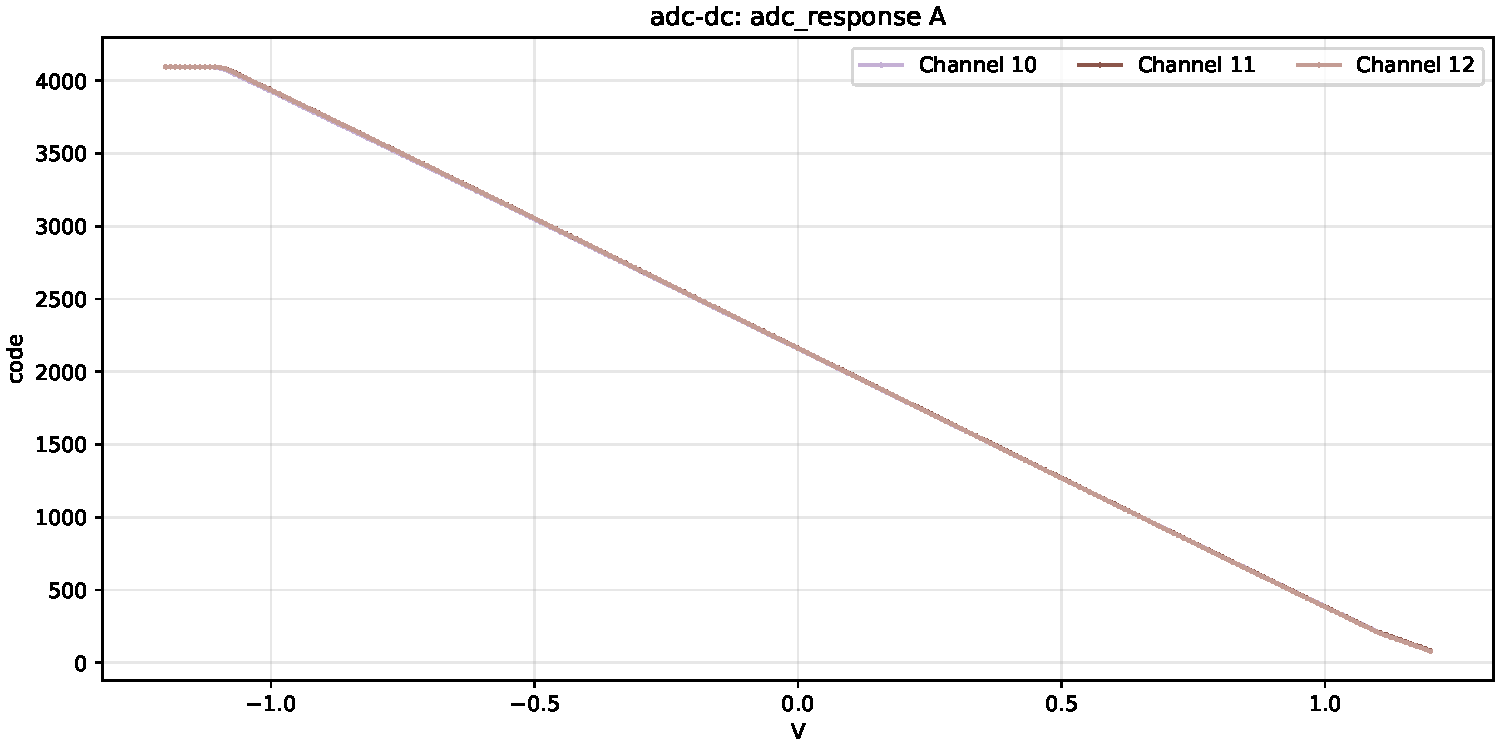
\includegraphics[width=\textwidth]{figures/figure-000.pdf}\end{center}
\begin{center}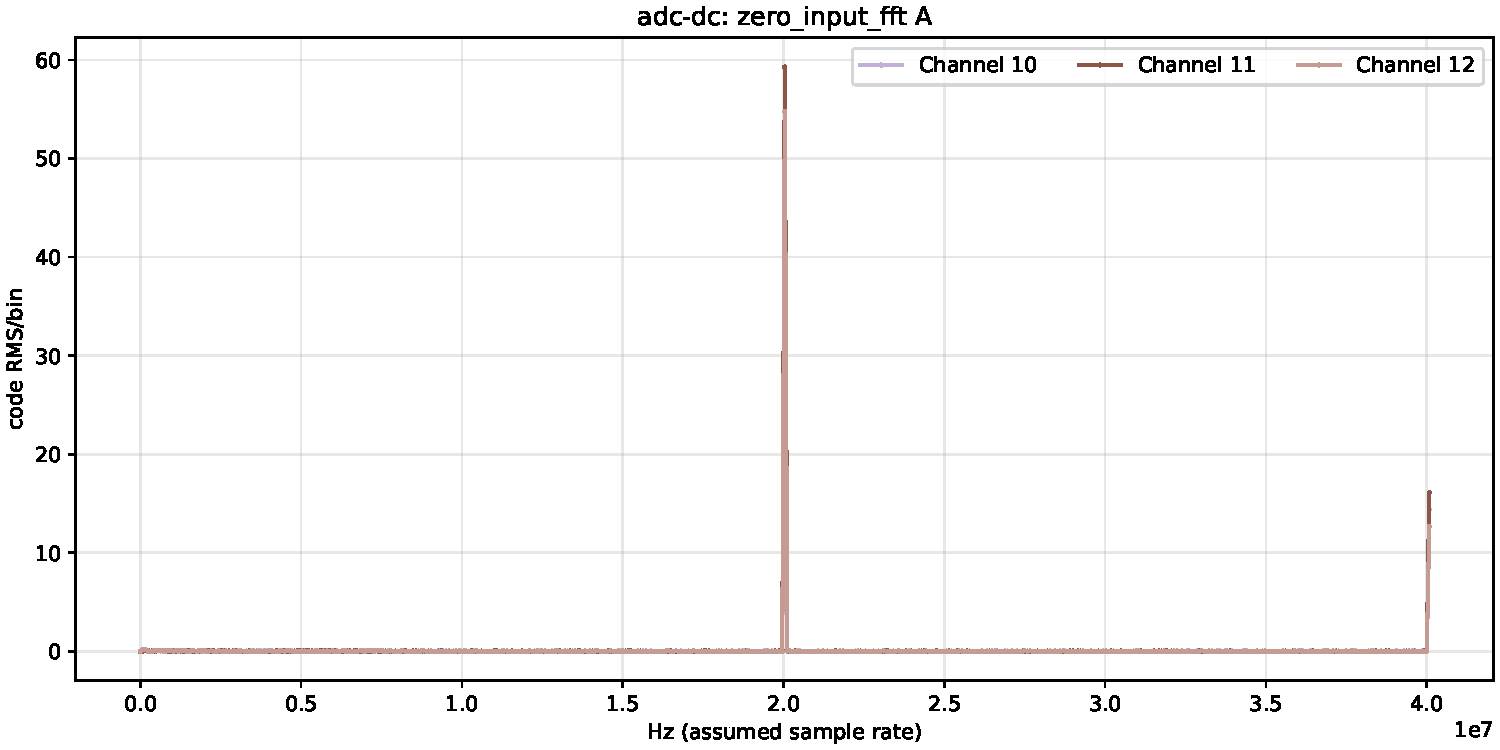
\includegraphics[width=\textwidth]{figures/figure-001.pdf}\end{center}
\begin{center}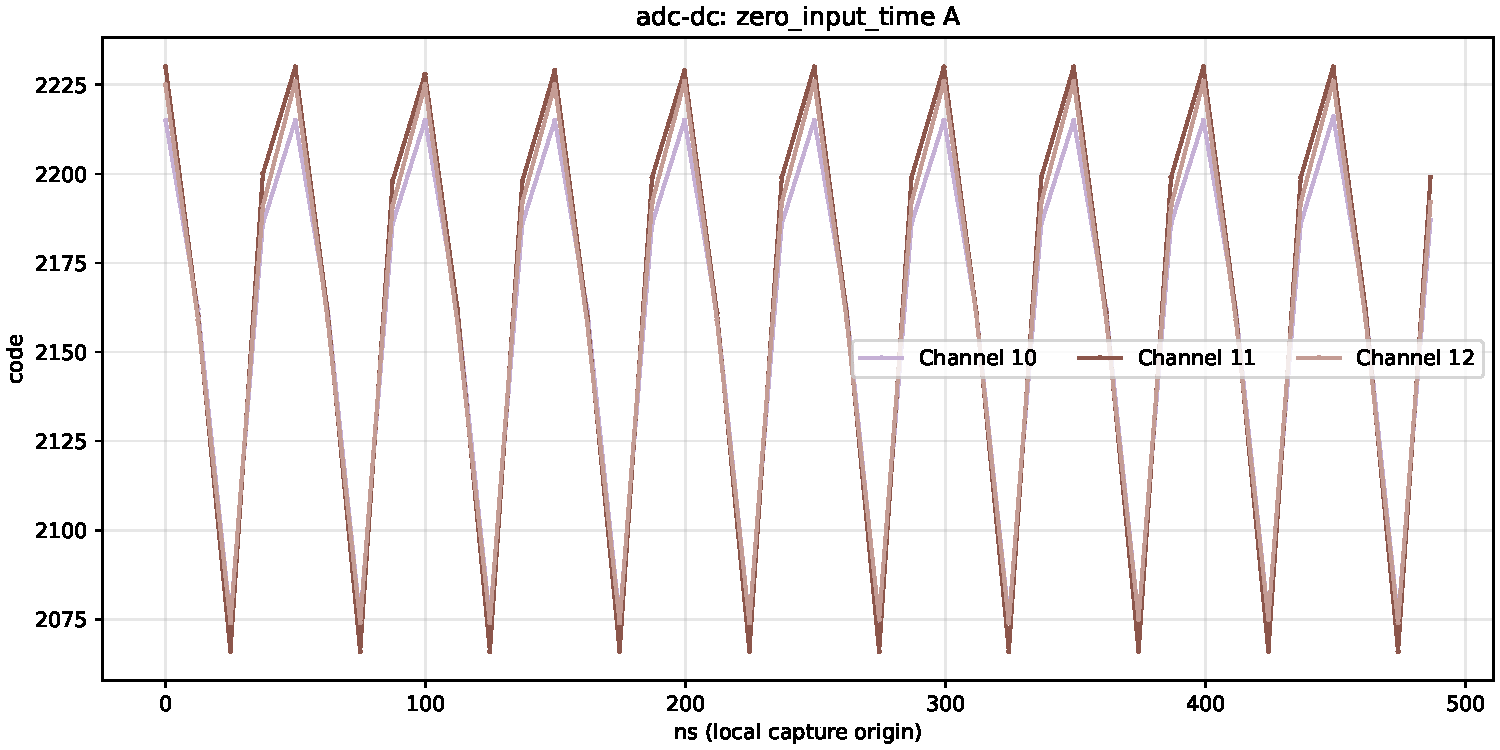
\includegraphics[width=\textwidth]{figures/figure-002.pdf}\end{center}
\begin{center}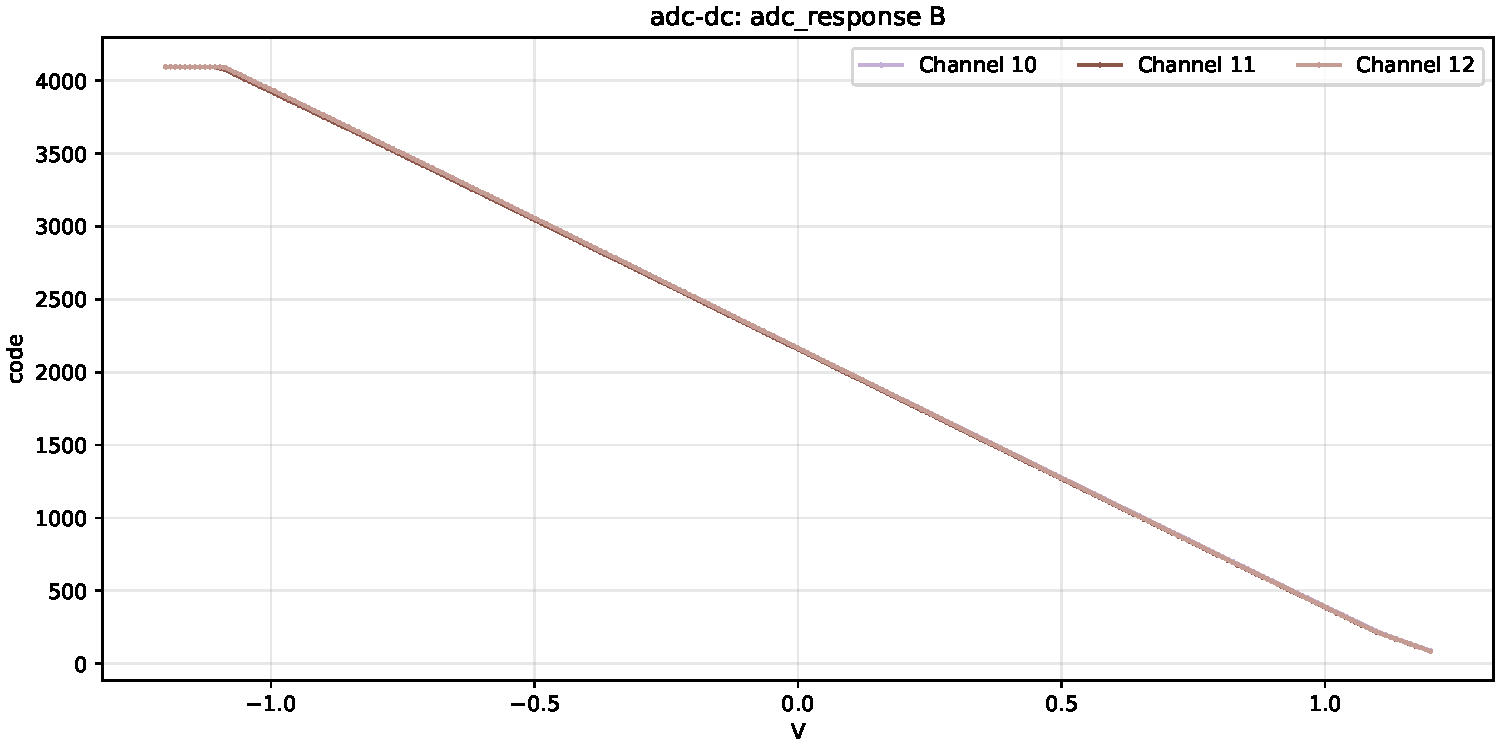
\includegraphics[width=\textwidth]{figures/figure-003.pdf}\end{center}
\begin{center}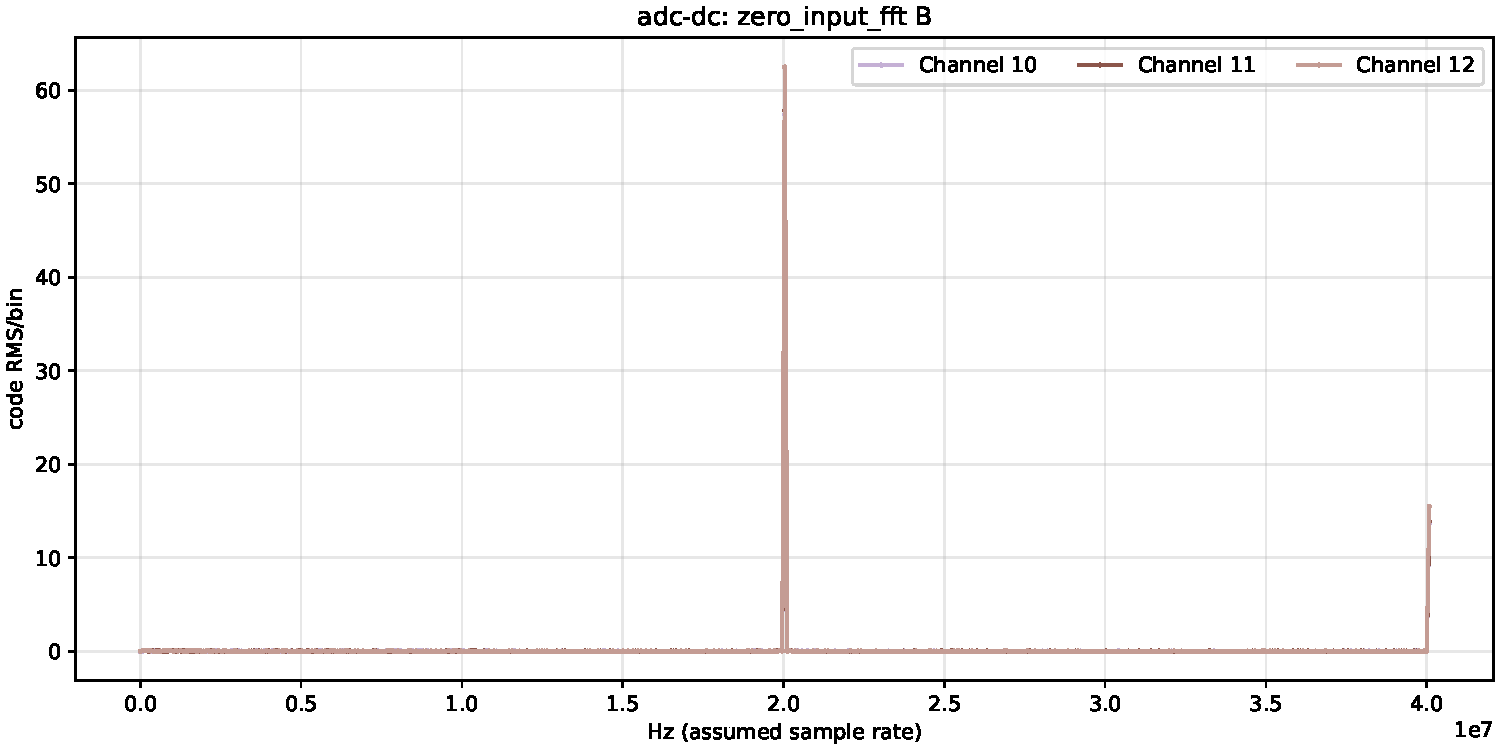
\includegraphics[width=\textwidth]{figures/figure-004.pdf}\end{center}
\begin{center}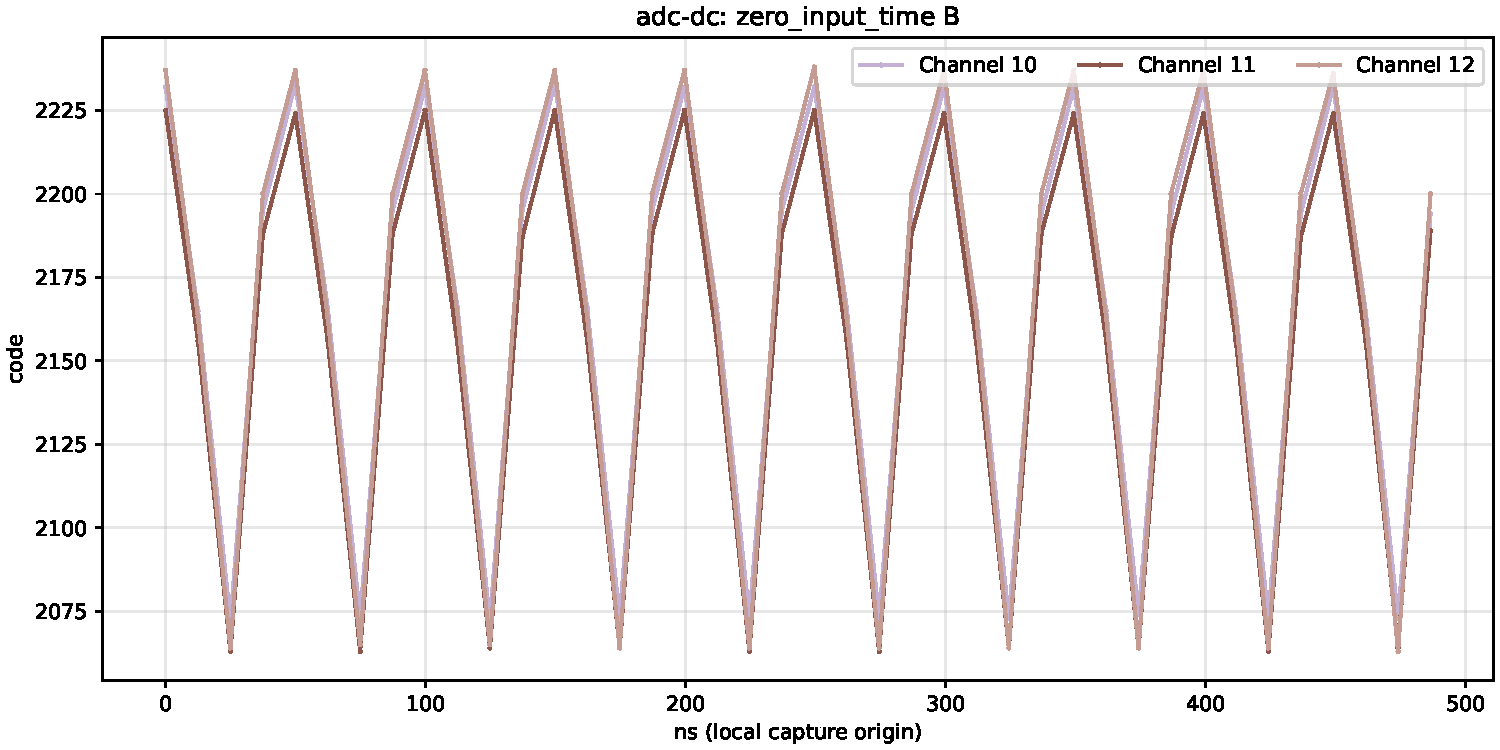
\includegraphics[width=\textwidth]{figures/figure-005.pdf}\end{center}
\begin{center}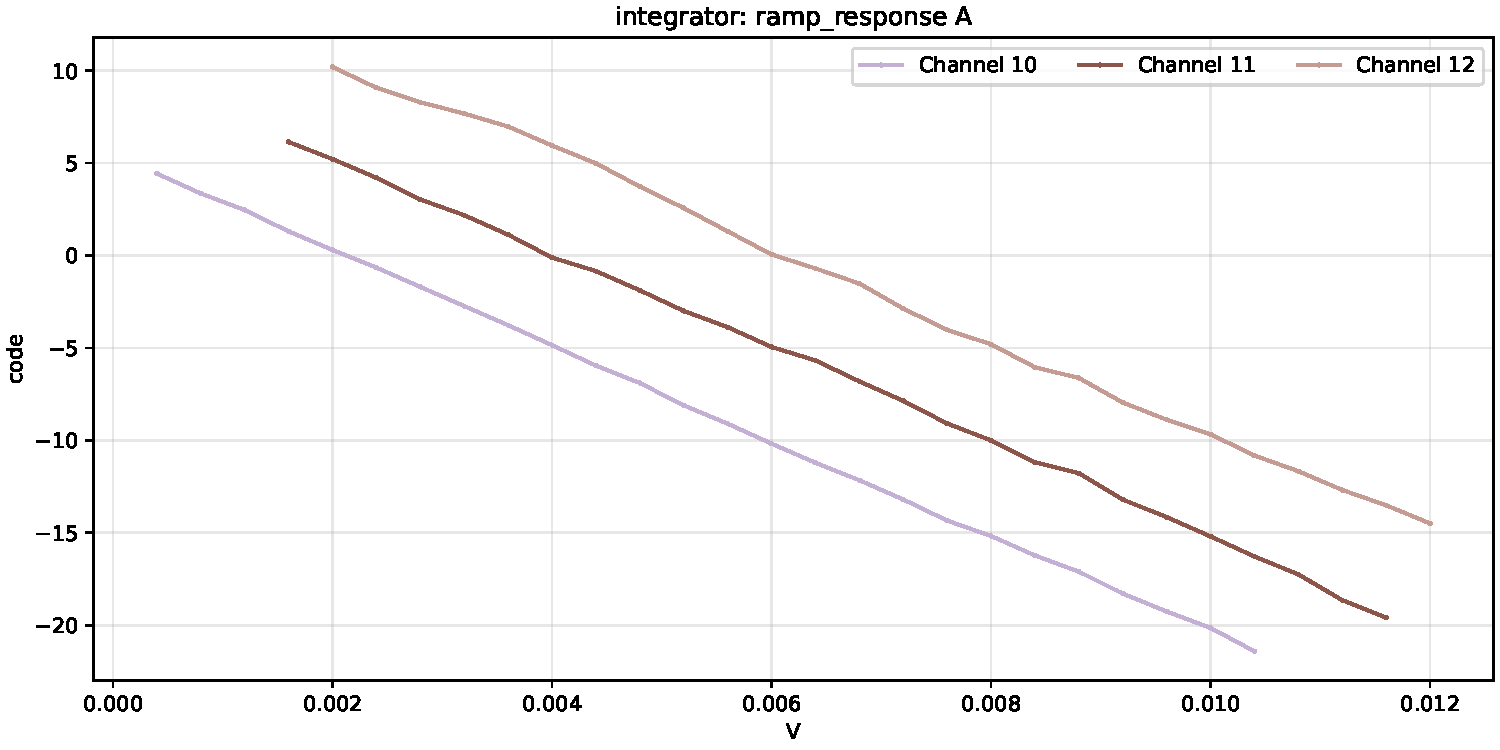
\includegraphics[width=\textwidth]{figures/figure-006.pdf}\end{center}
\begin{center}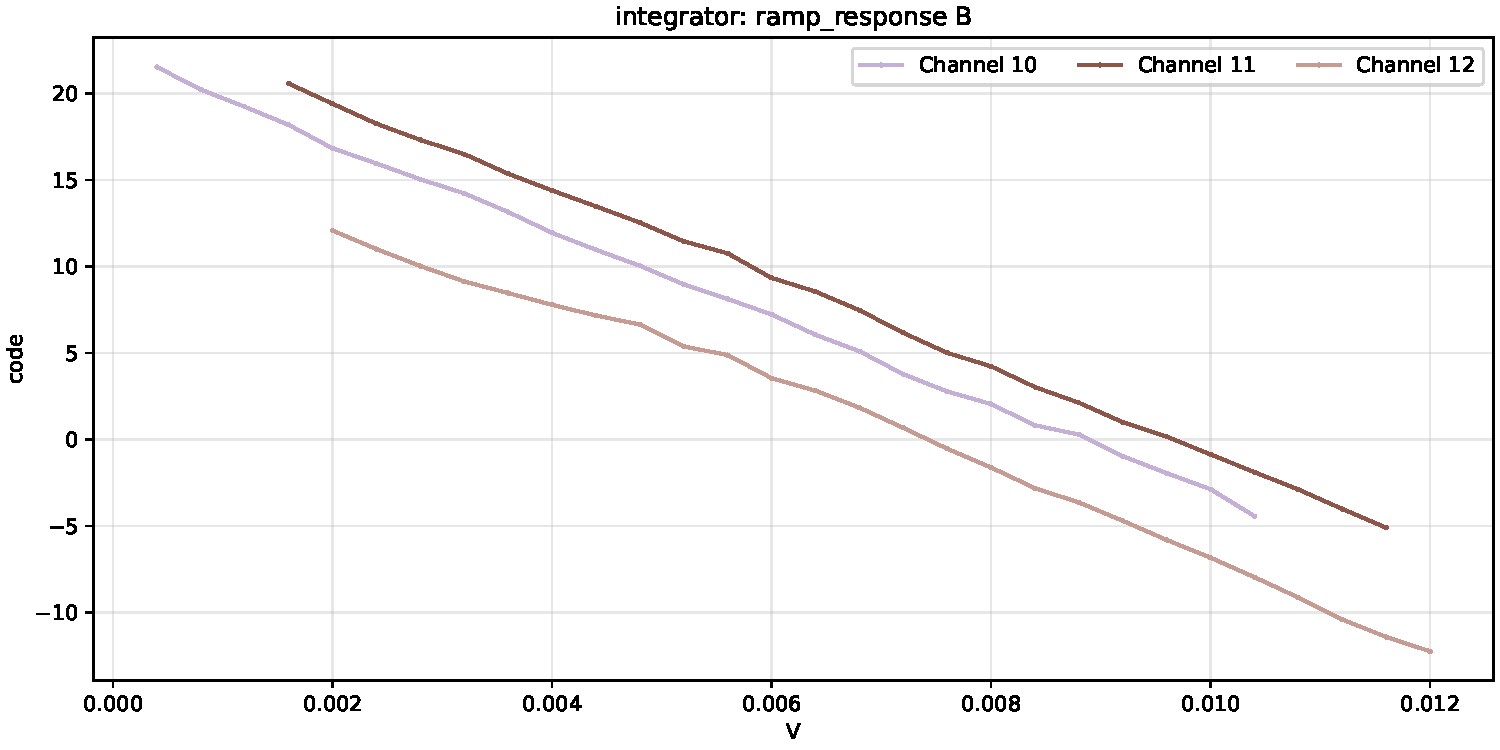
\includegraphics[width=\textwidth]{figures/figure-007.pdf}\end{center}
\begin{center}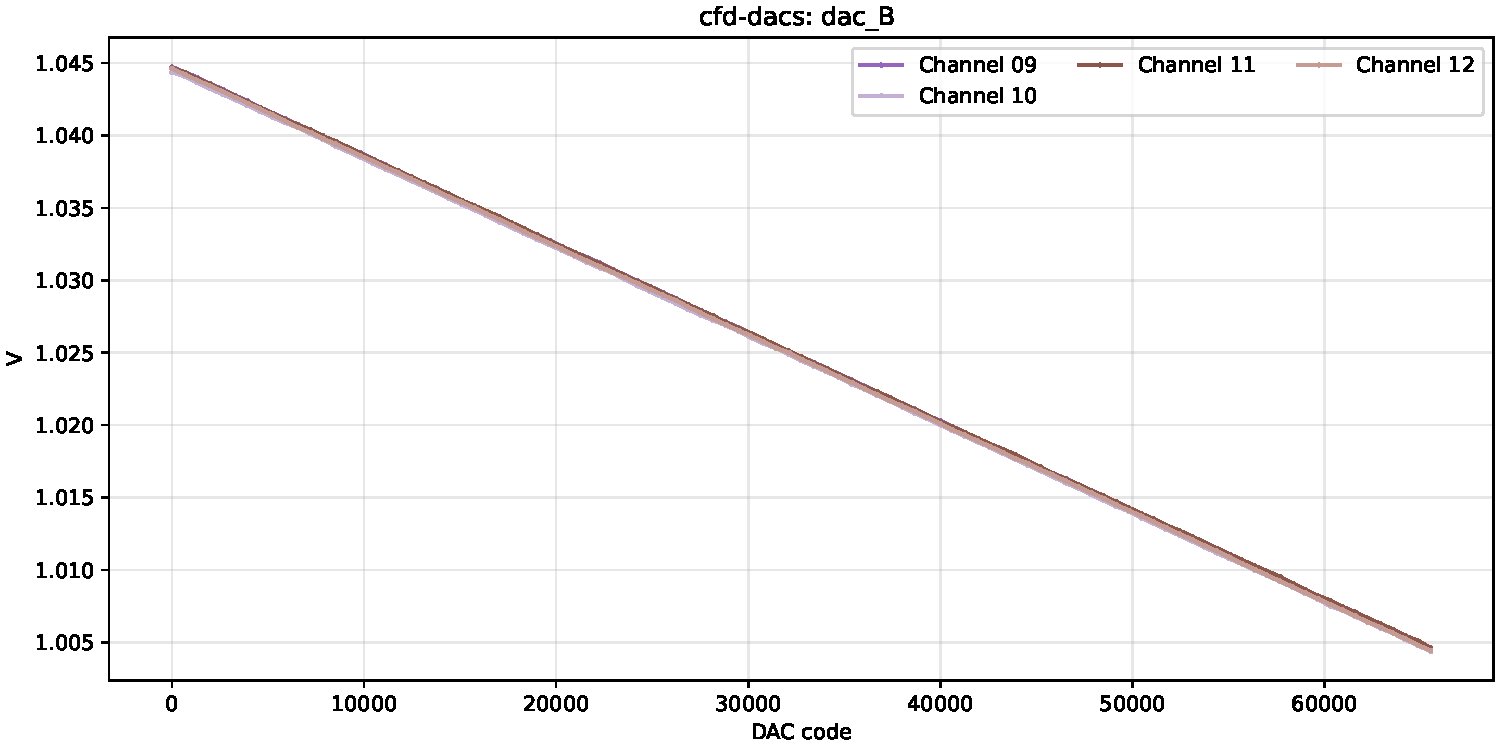
\includegraphics[width=\textwidth]{figures/figure-008.pdf}\end{center}
\begin{center}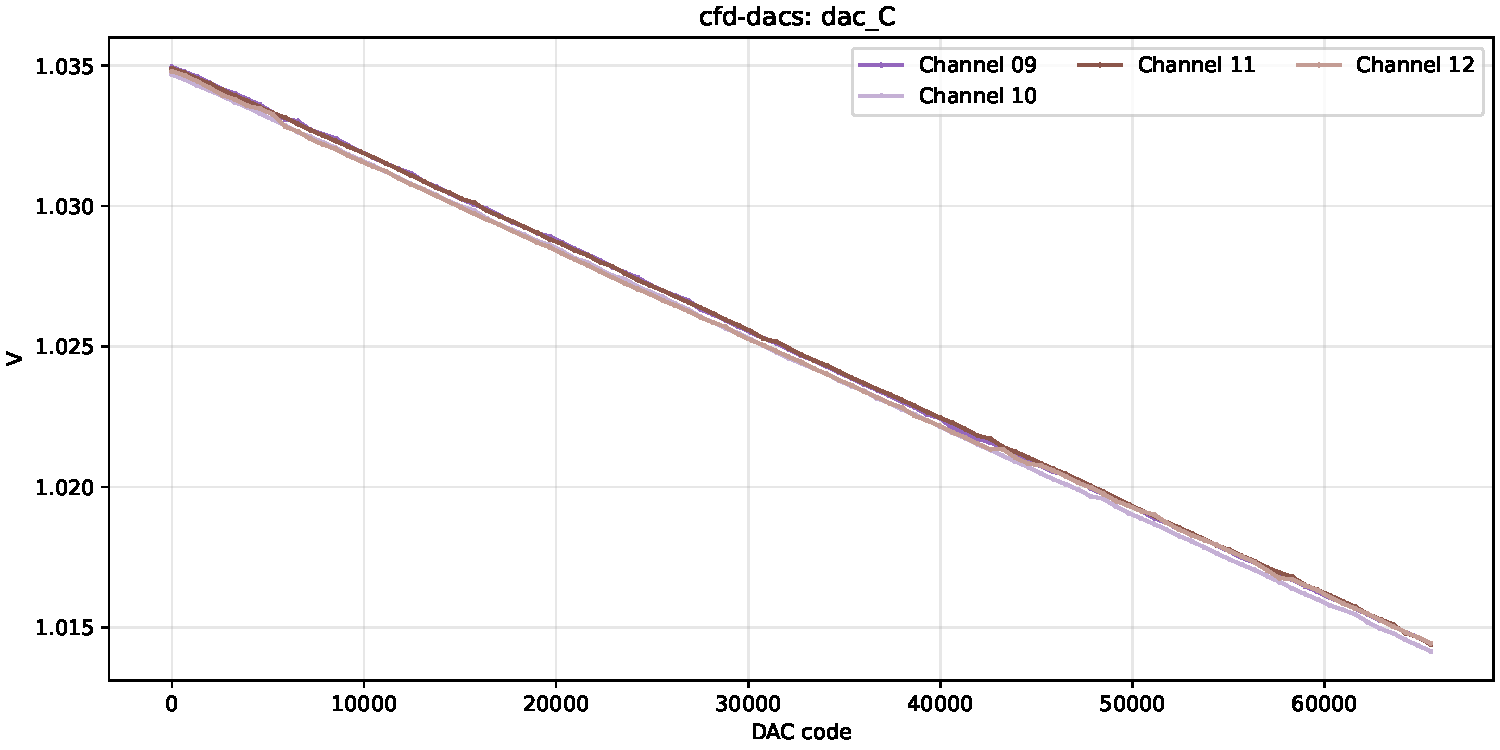
\includegraphics[width=\textwidth]{figures/figure-009.pdf}\end{center}
\begin{center}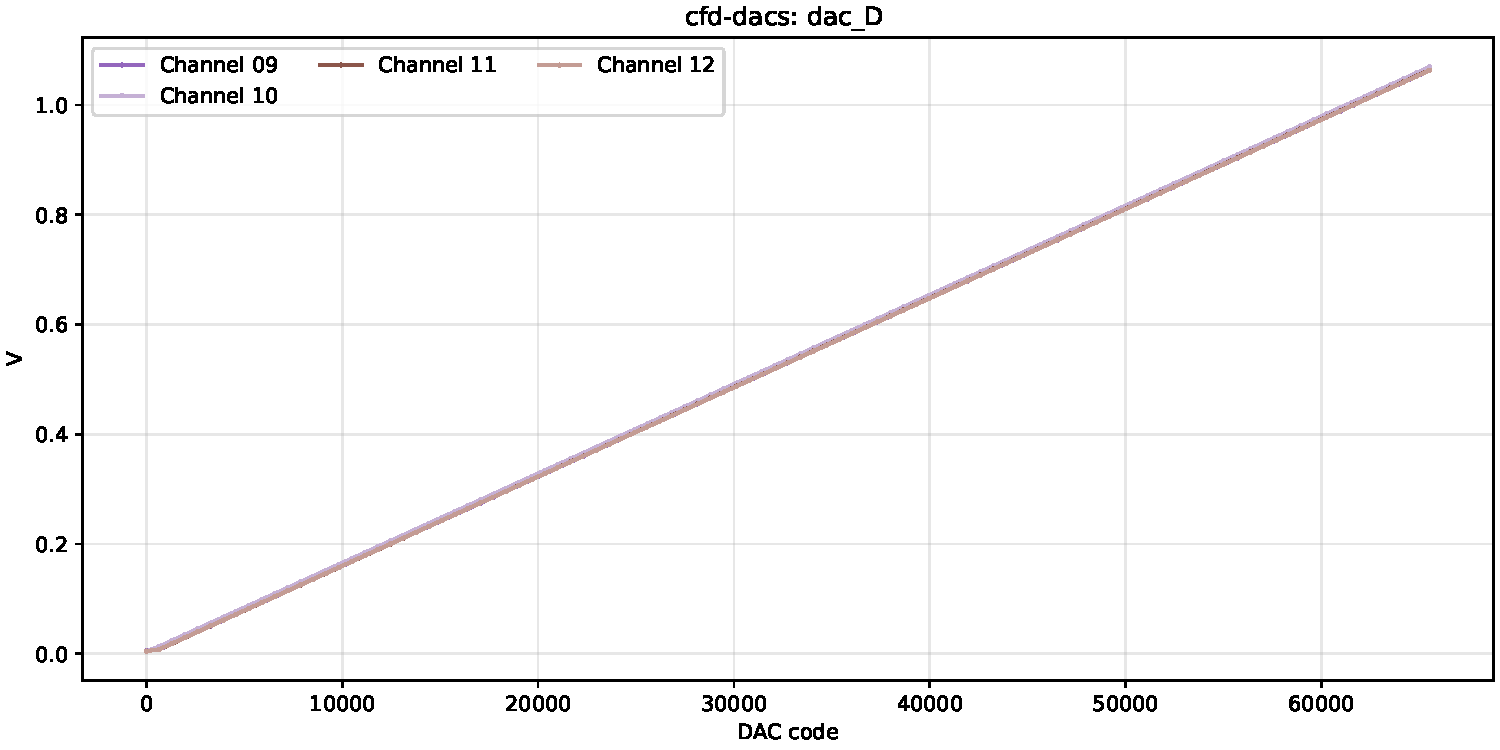
\includegraphics[width=\textwidth]{figures/figure-010.pdf}\end{center}
\begin{center}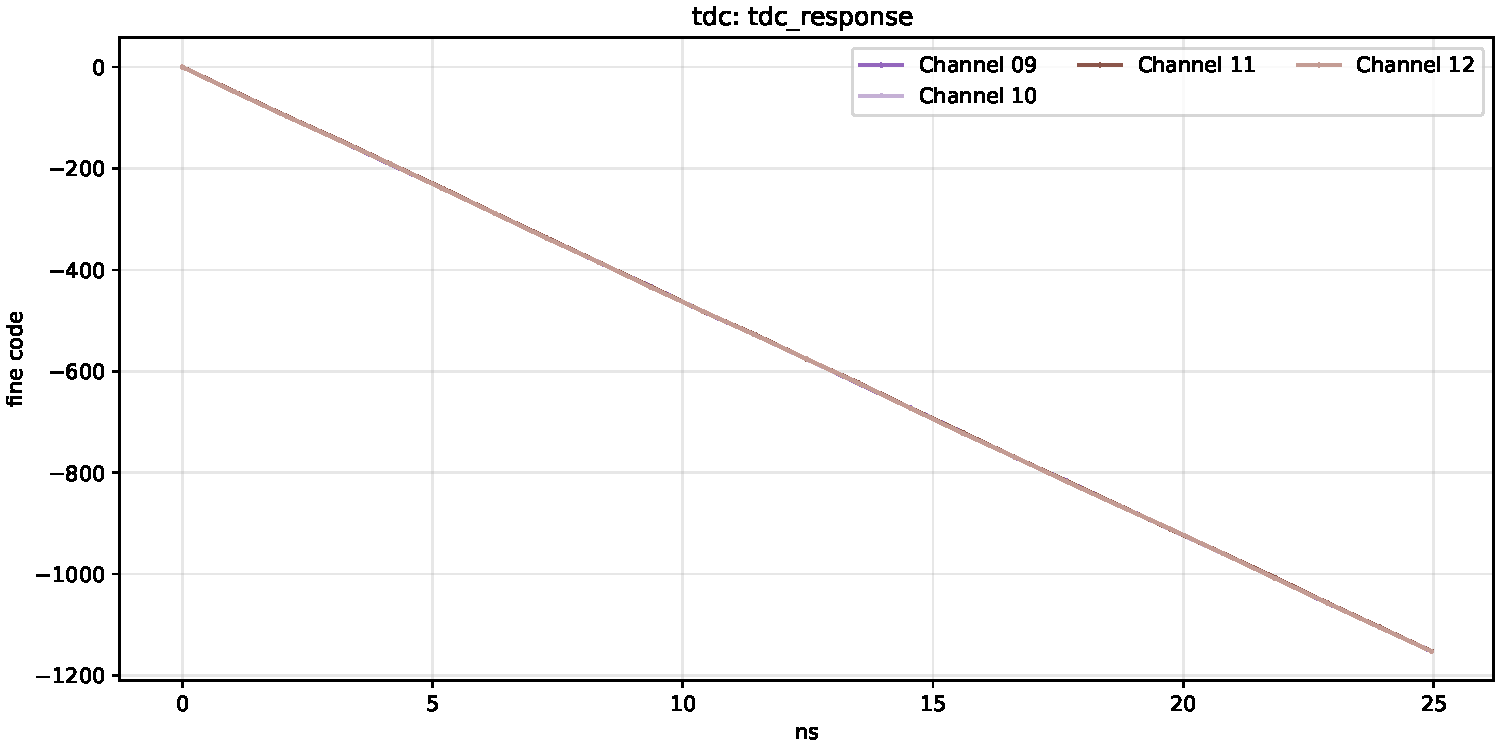
\includegraphics[width=\textwidth]{figures/figure-011.pdf}\end{center}
\begin{center}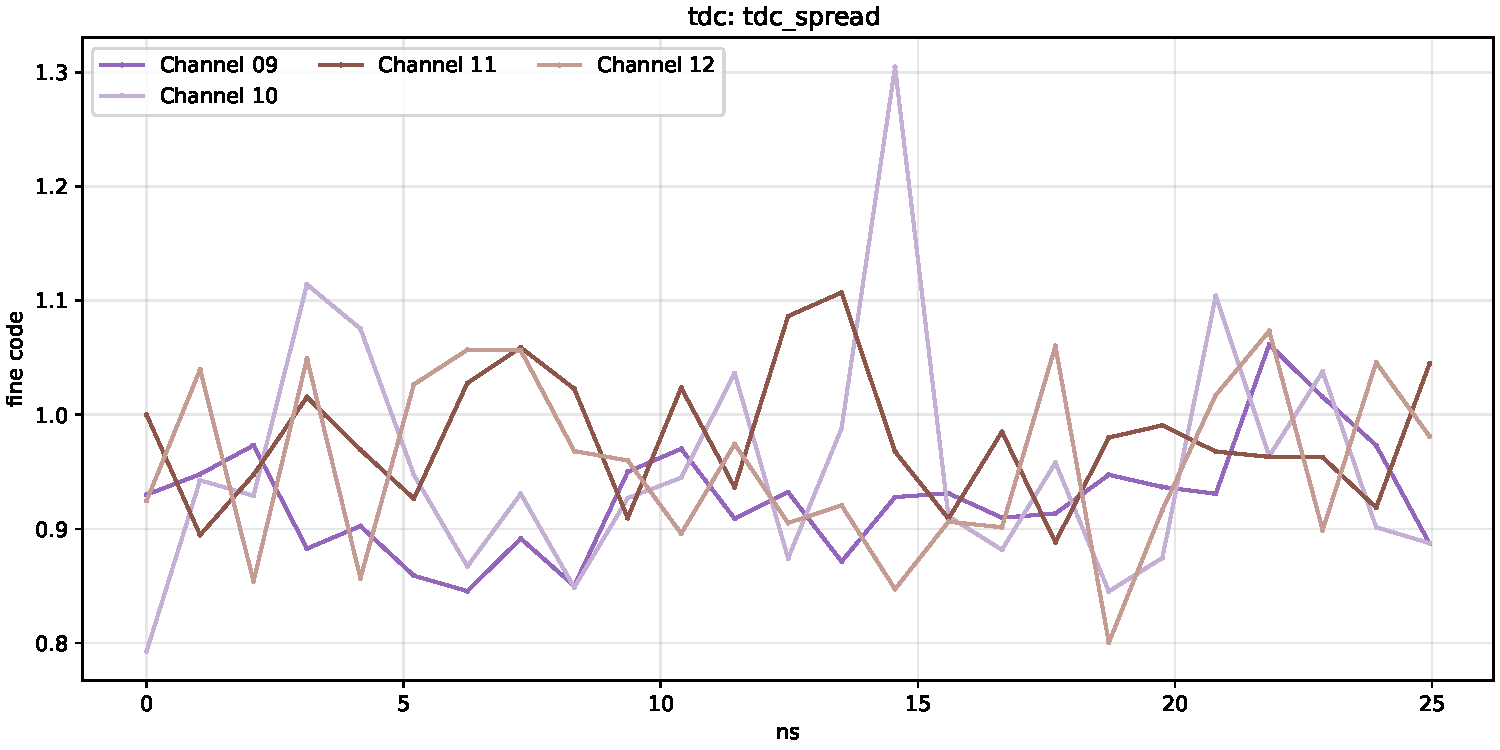
\includegraphics[width=\textwidth]{figures/figure-012.pdf}\end{center}
\begin{center}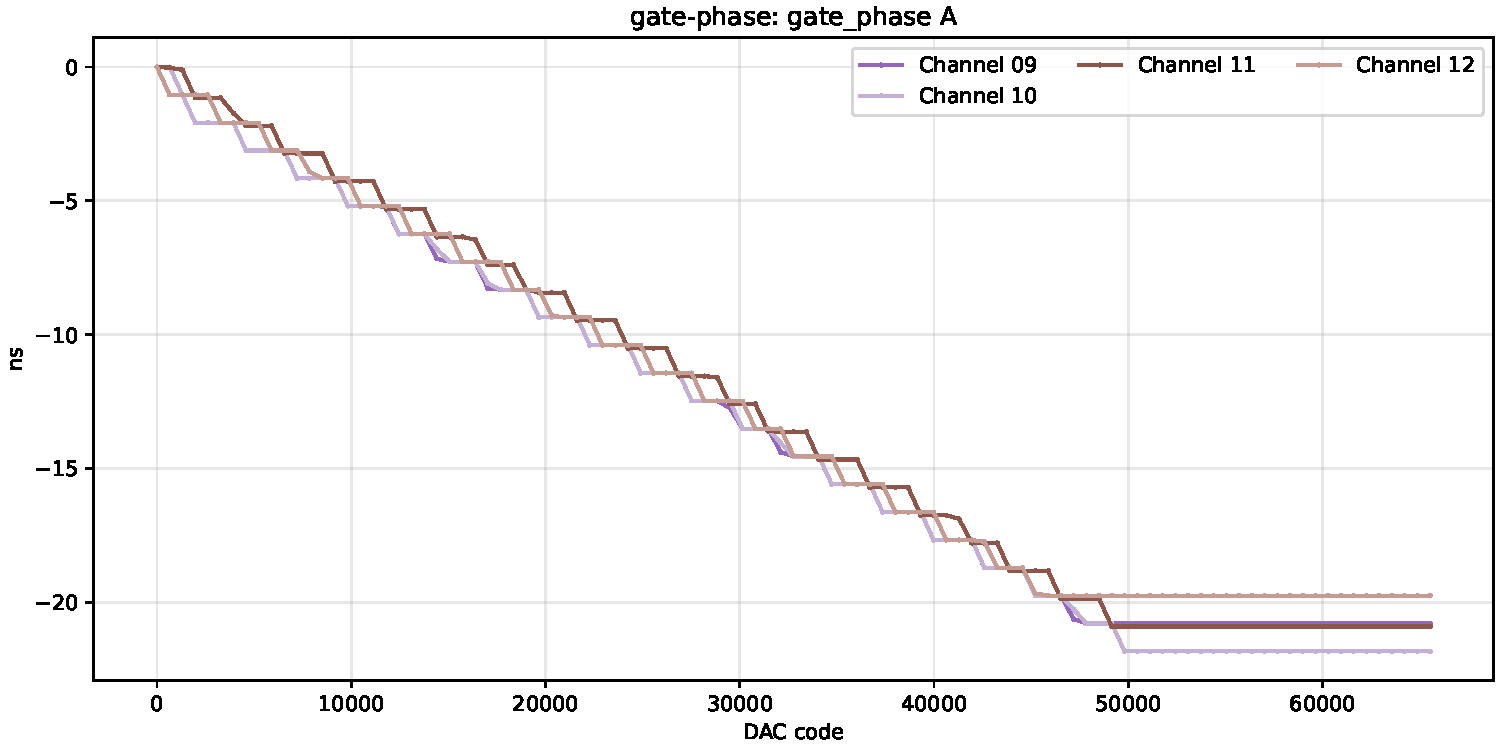
\includegraphics[width=\textwidth]{figures/figure-013.pdf}\end{center}
\begin{center}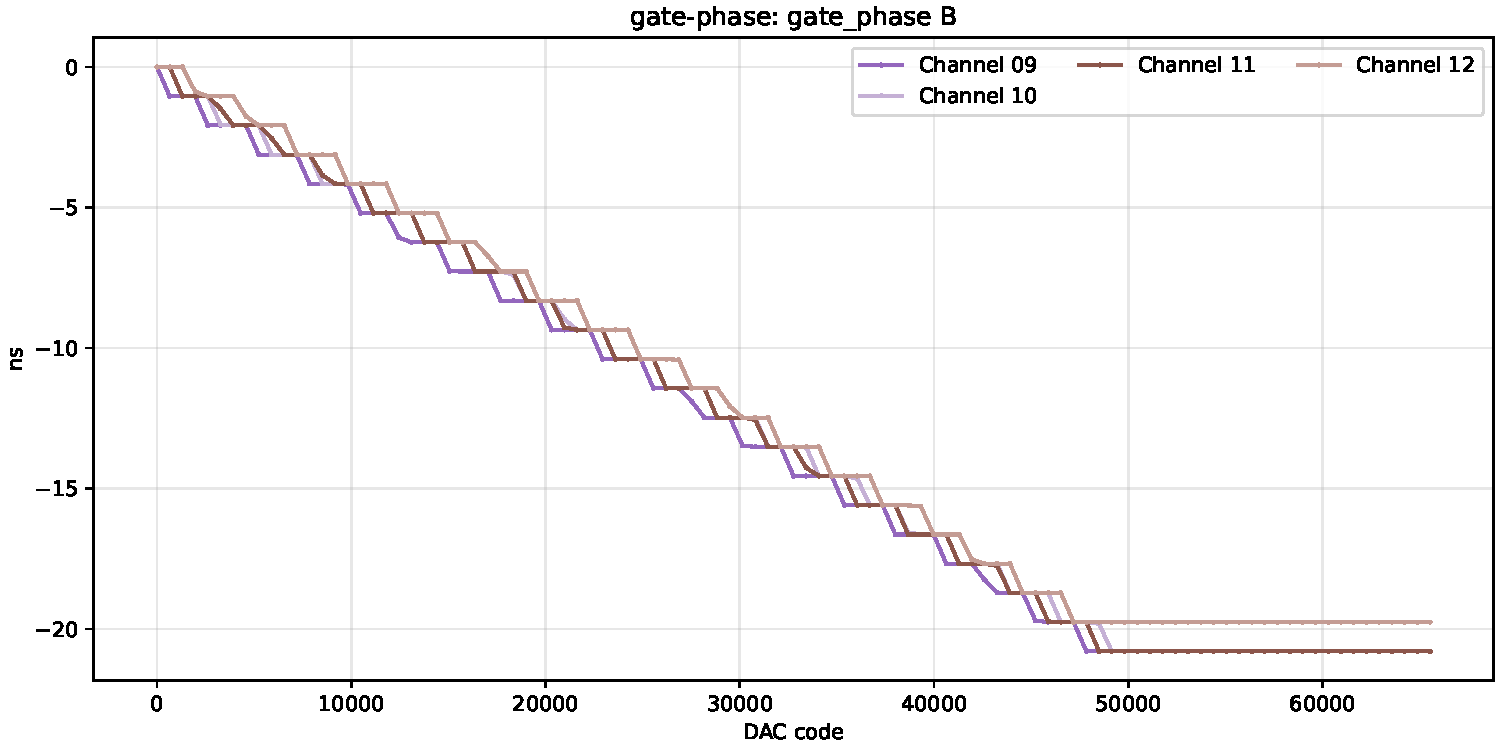
\includegraphics[width=\textwidth]{figures/figure-014.pdf}\end{center}
\begin{center}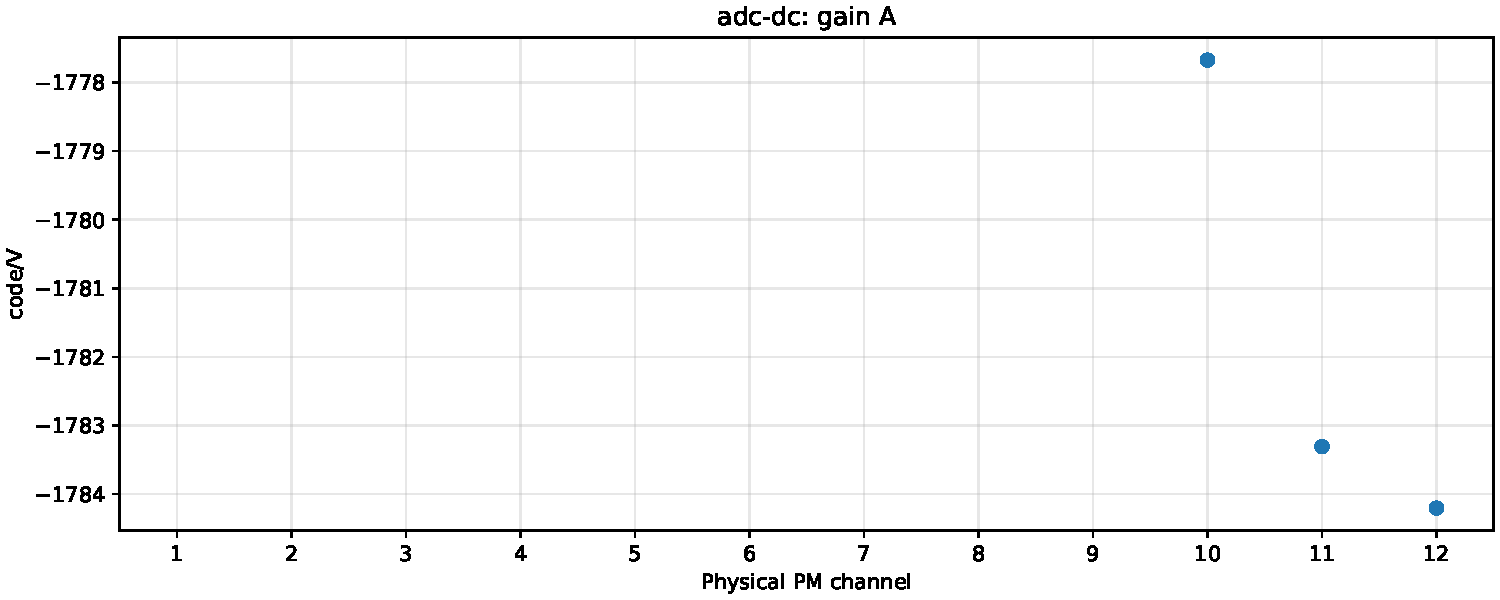
\includegraphics[width=\textwidth]{figures/figure-015.pdf}\end{center}
\begin{center}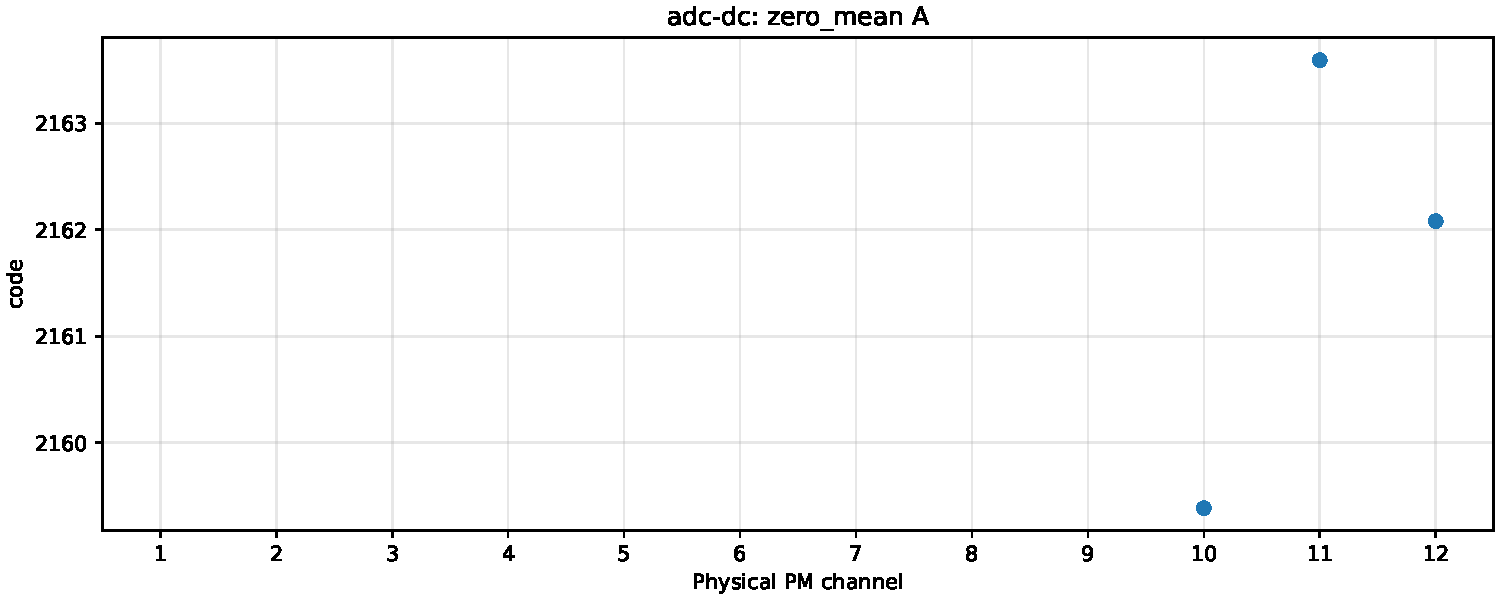
\includegraphics[width=\textwidth]{figures/figure-016.pdf}\end{center}
\begin{center}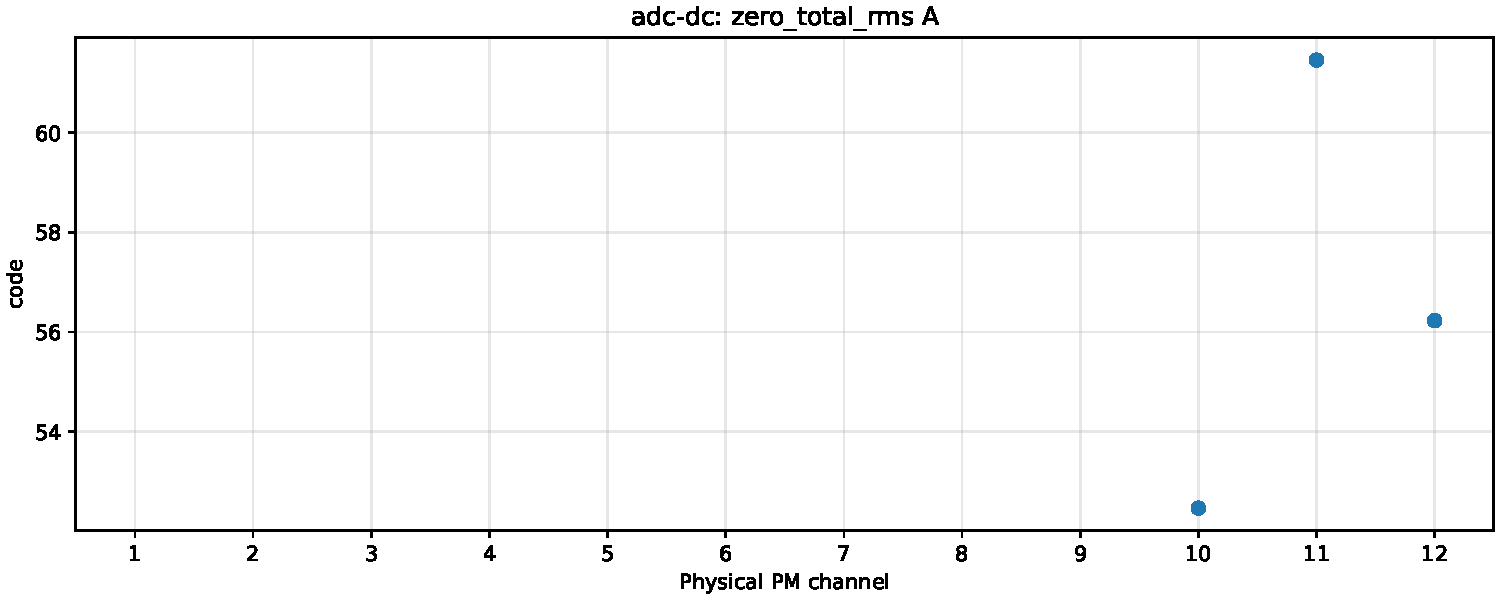
\includegraphics[width=\textwidth]{figures/figure-017.pdf}\end{center}
\begin{center}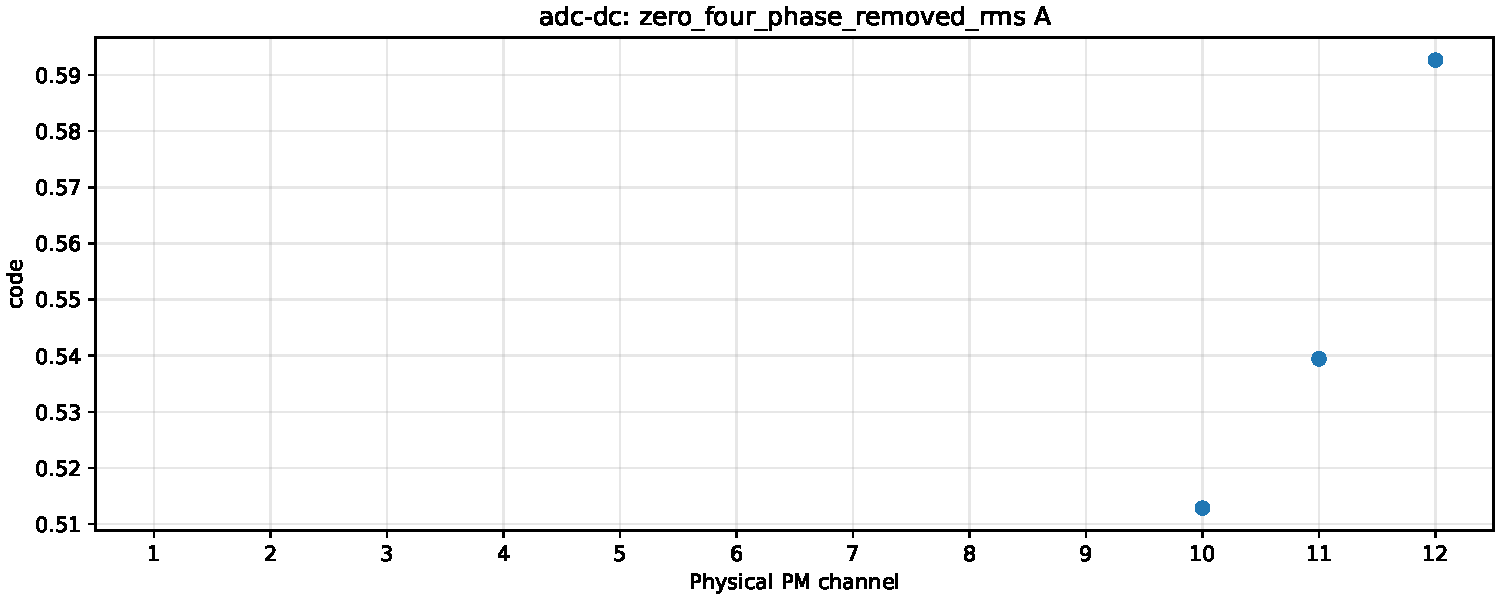
\includegraphics[width=\textwidth]{figures/figure-018.pdf}\end{center}
\begin{center}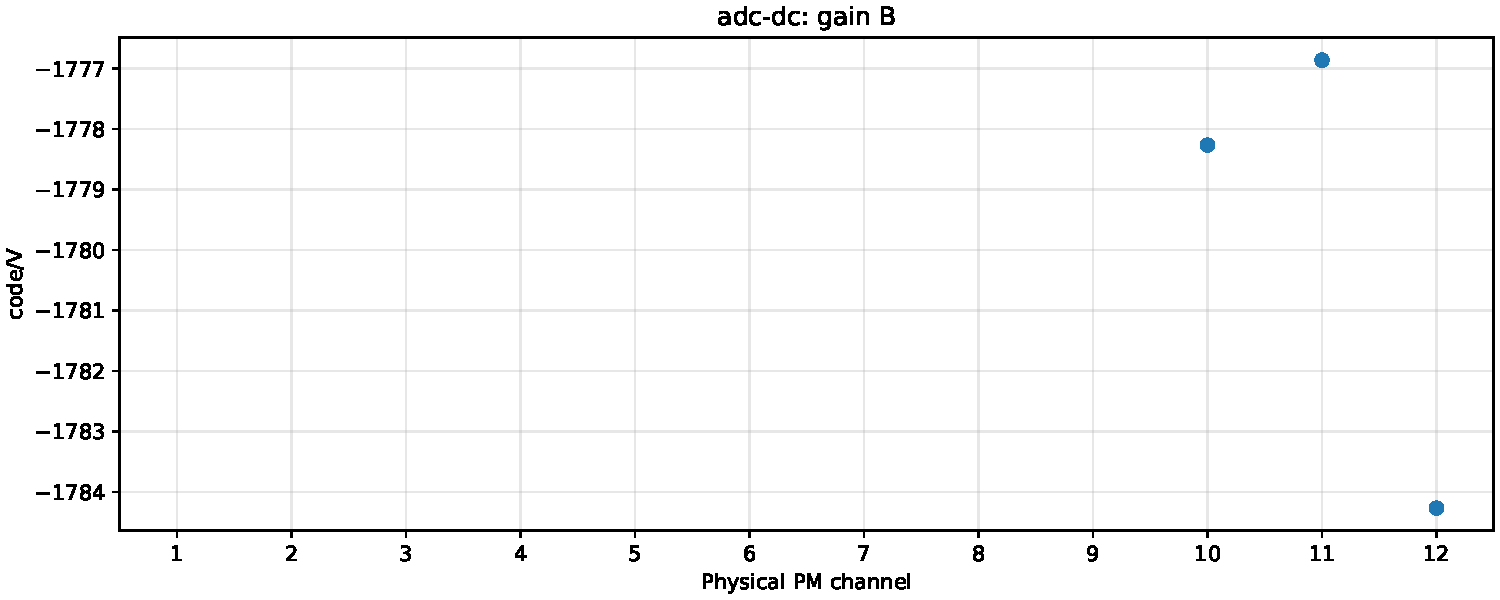
\includegraphics[width=\textwidth]{figures/figure-019.pdf}\end{center}
\begin{center}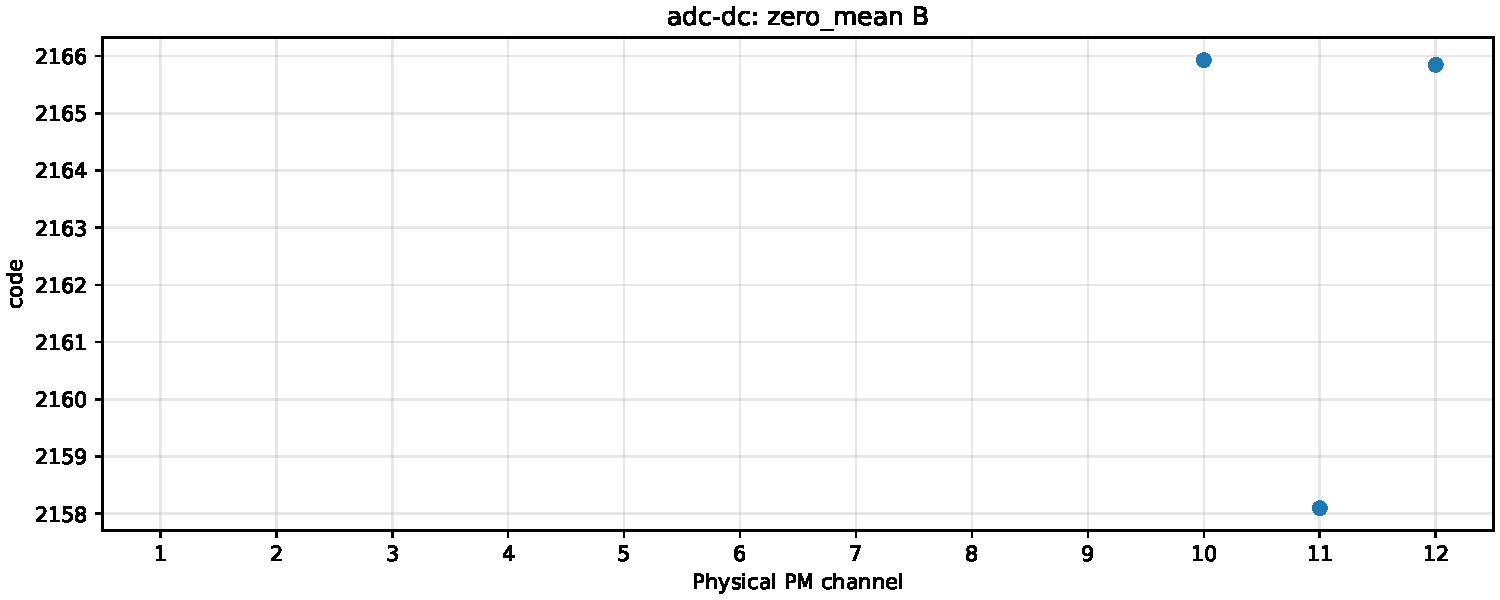
\includegraphics[width=\textwidth]{figures/figure-020.pdf}\end{center}
\begin{center}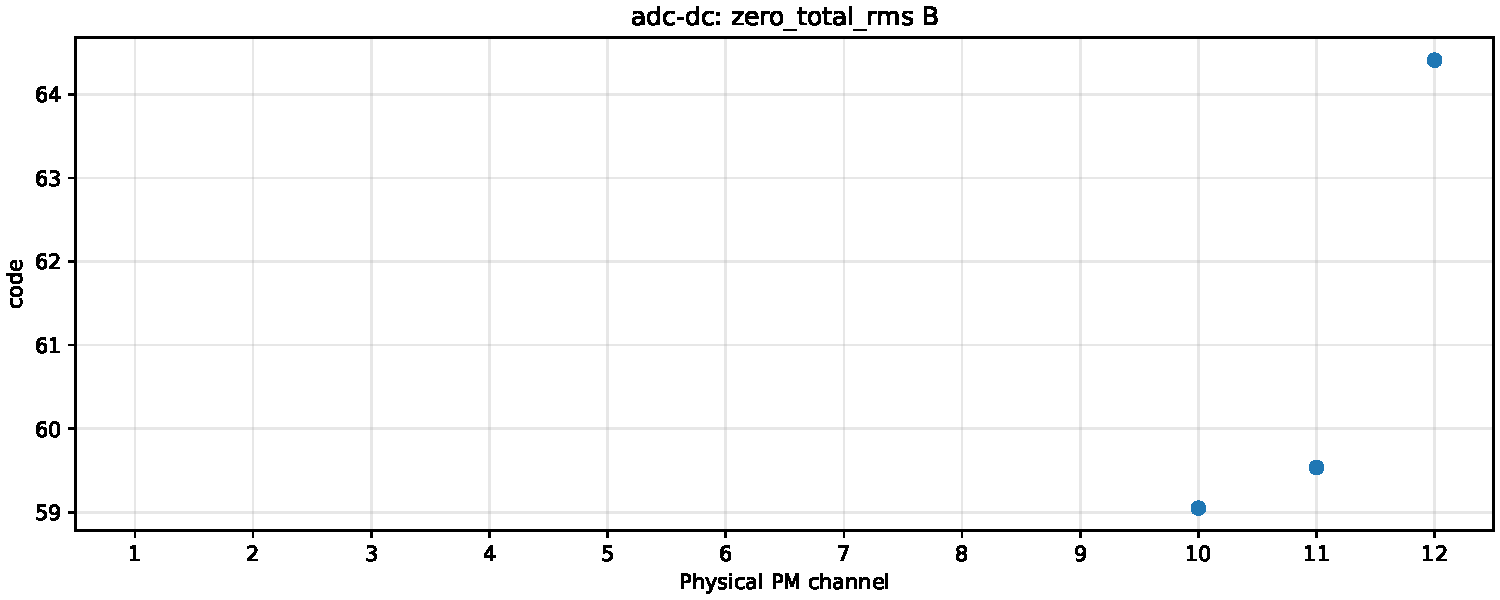
\includegraphics[width=\textwidth]{figures/figure-021.pdf}\end{center}
\begin{center}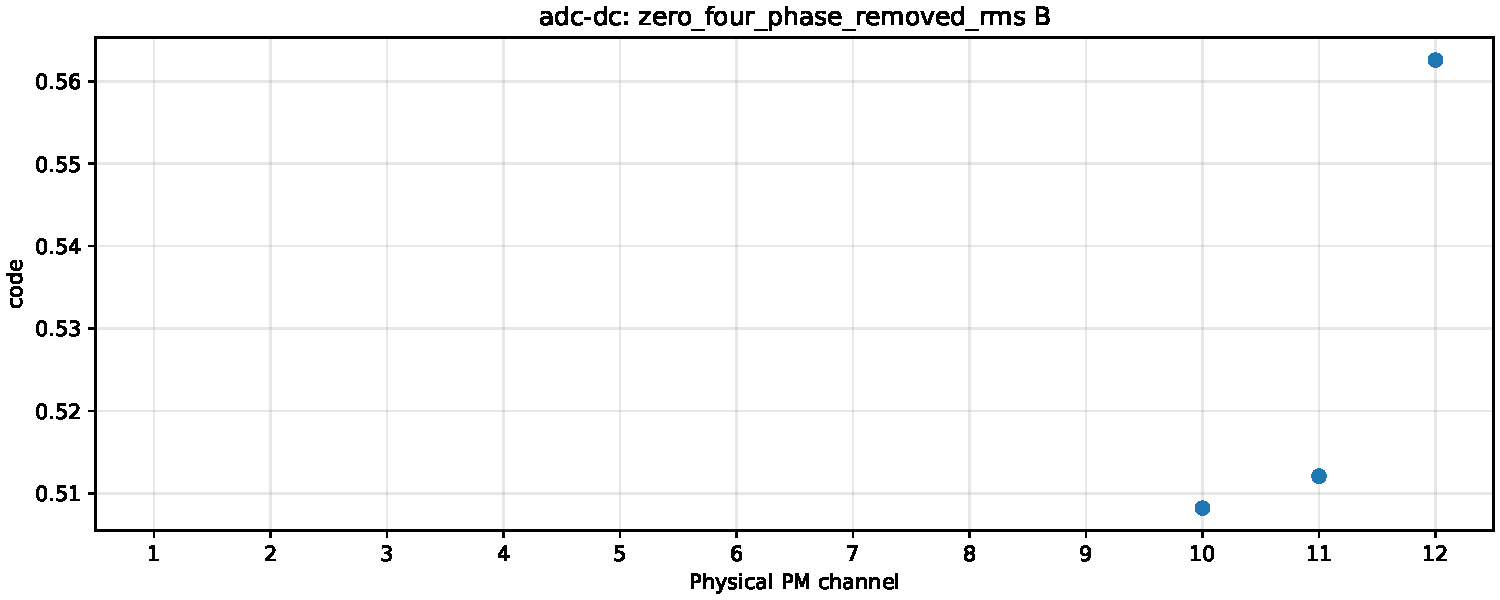
\includegraphics[width=\textwidth]{figures/figure-022.pdf}\end{center}
\begin{center}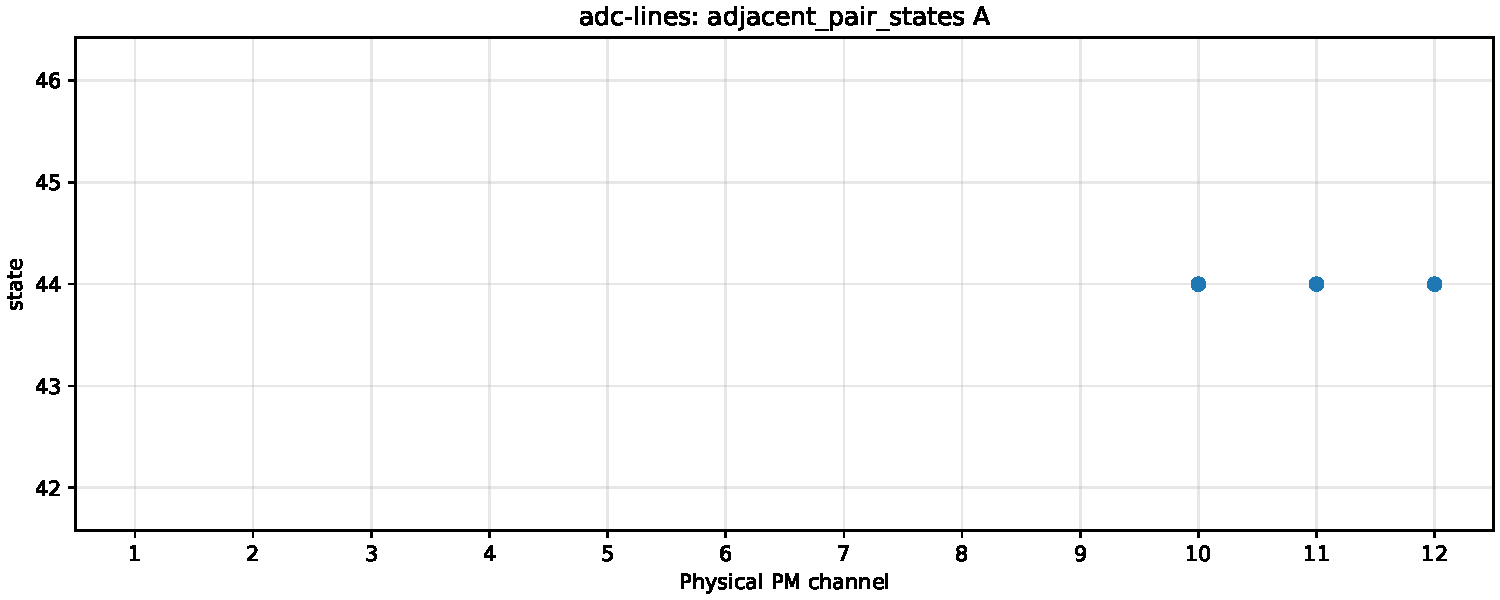
\includegraphics[width=\textwidth]{figures/figure-023.pdf}\end{center}
\begin{center}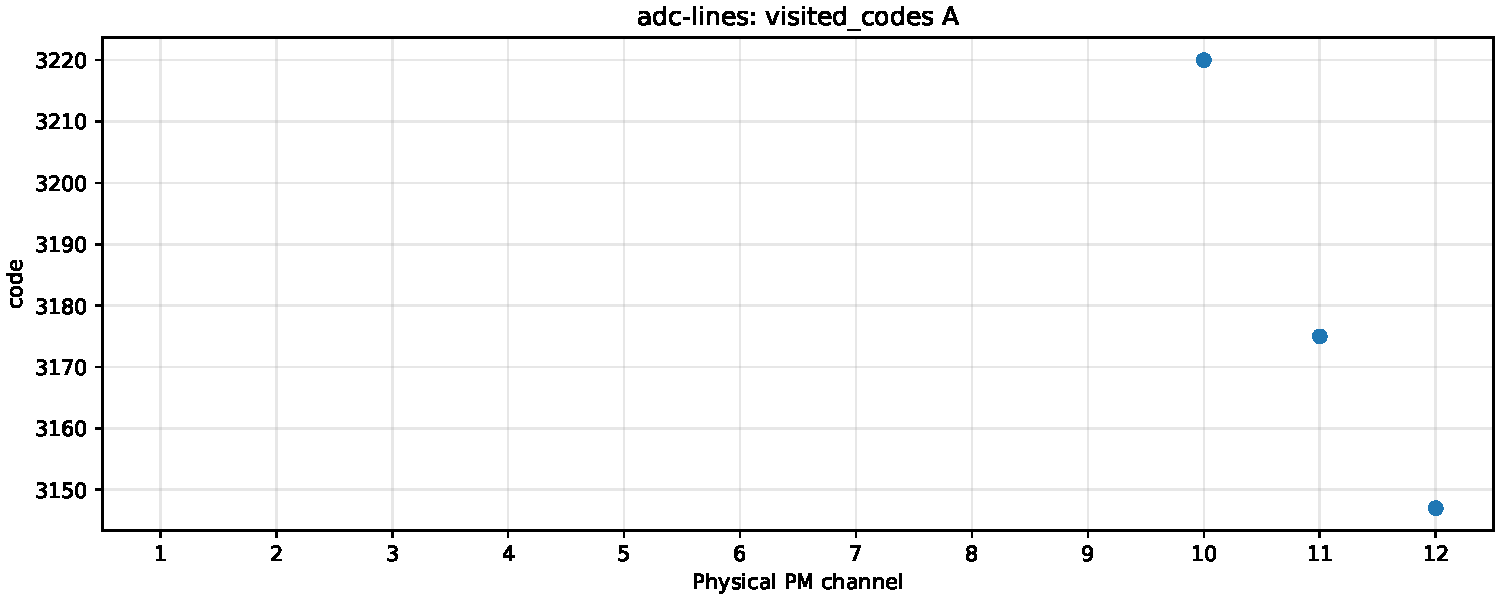
\includegraphics[width=\textwidth]{figures/figure-024.pdf}\end{center}
\begin{center}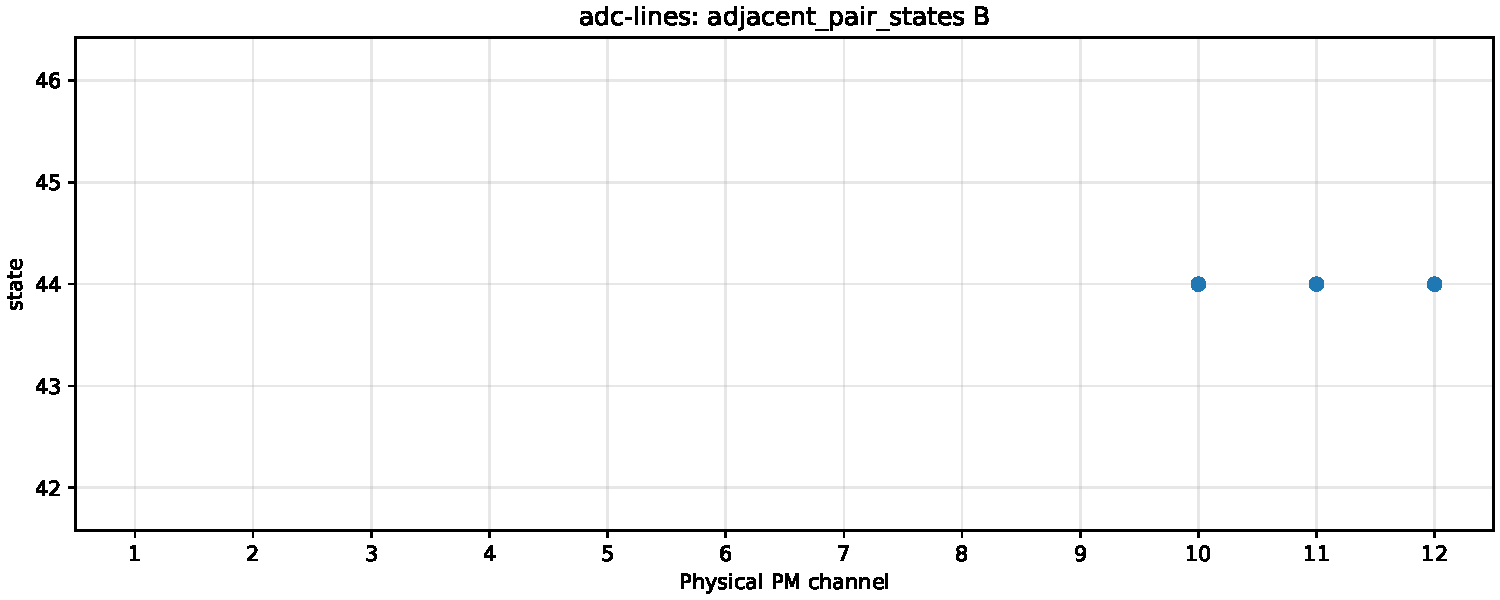
\includegraphics[width=\textwidth]{figures/figure-025.pdf}\end{center}
\begin{center}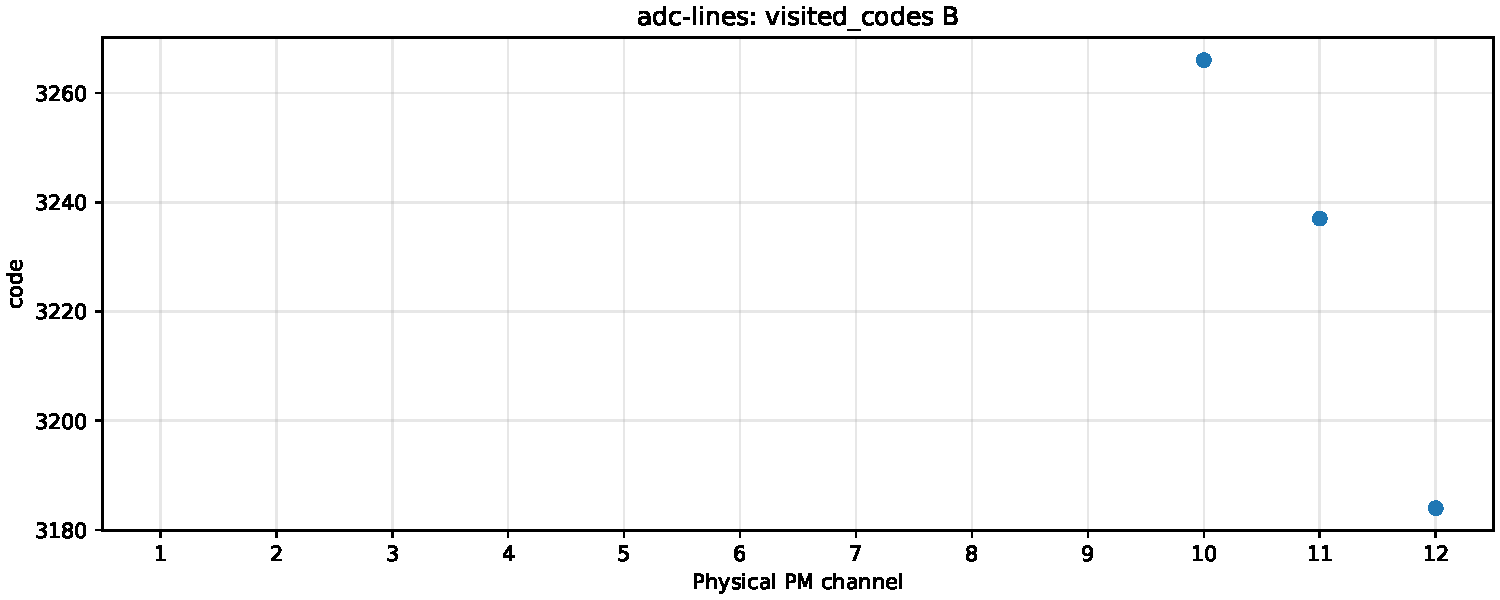
\includegraphics[width=\textwidth]{figures/figure-026.pdf}\end{center}
\begin{center}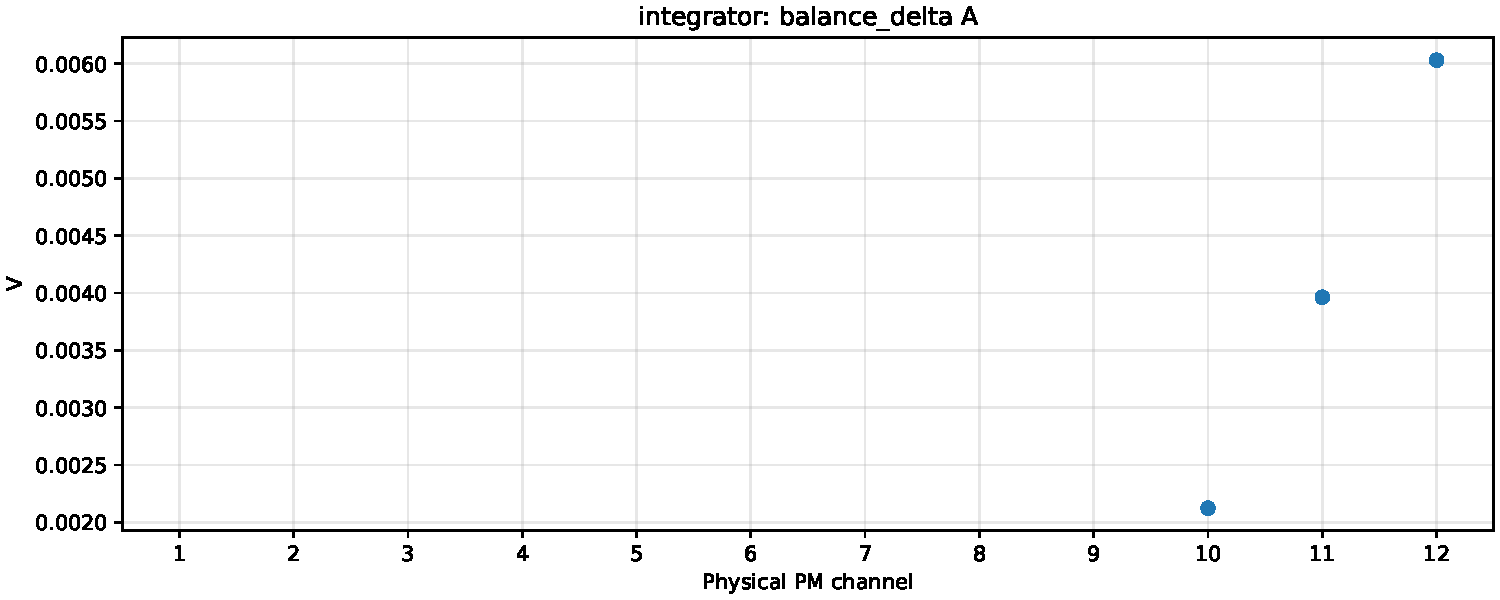
\includegraphics[width=\textwidth]{figures/figure-027.pdf}\end{center}
\begin{center}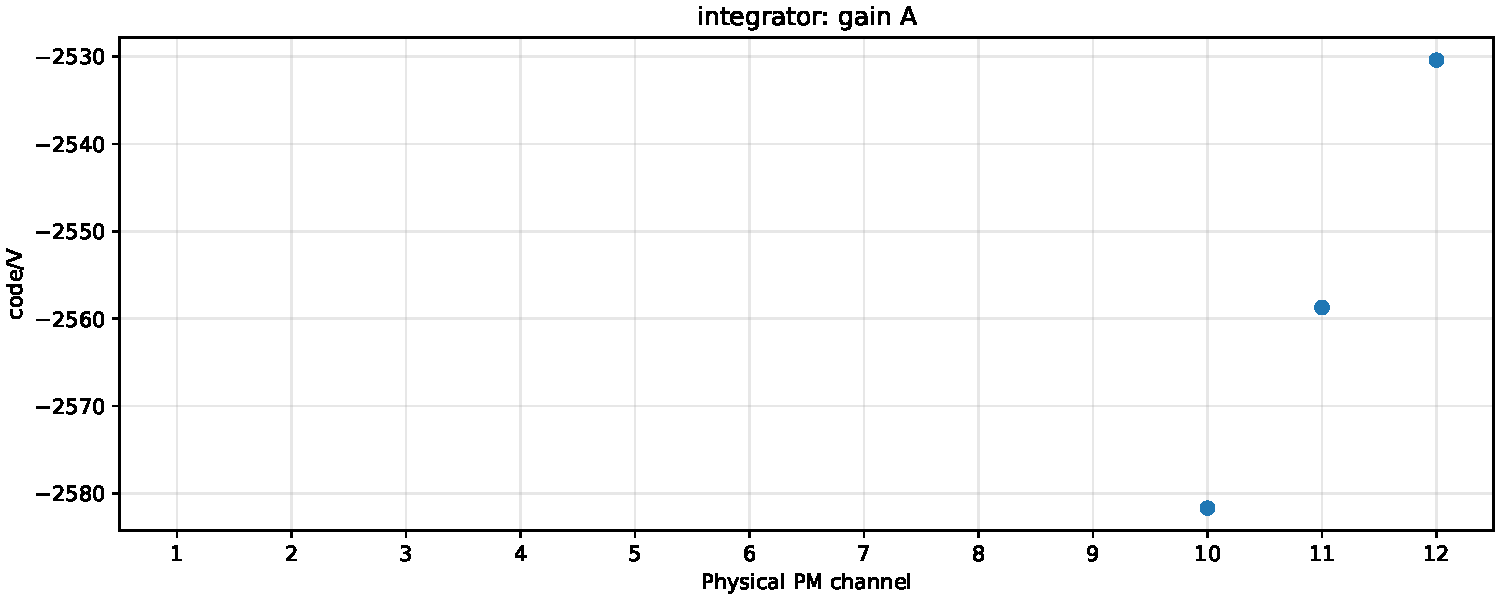
\includegraphics[width=\textwidth]{figures/figure-028.pdf}\end{center}
\begin{center}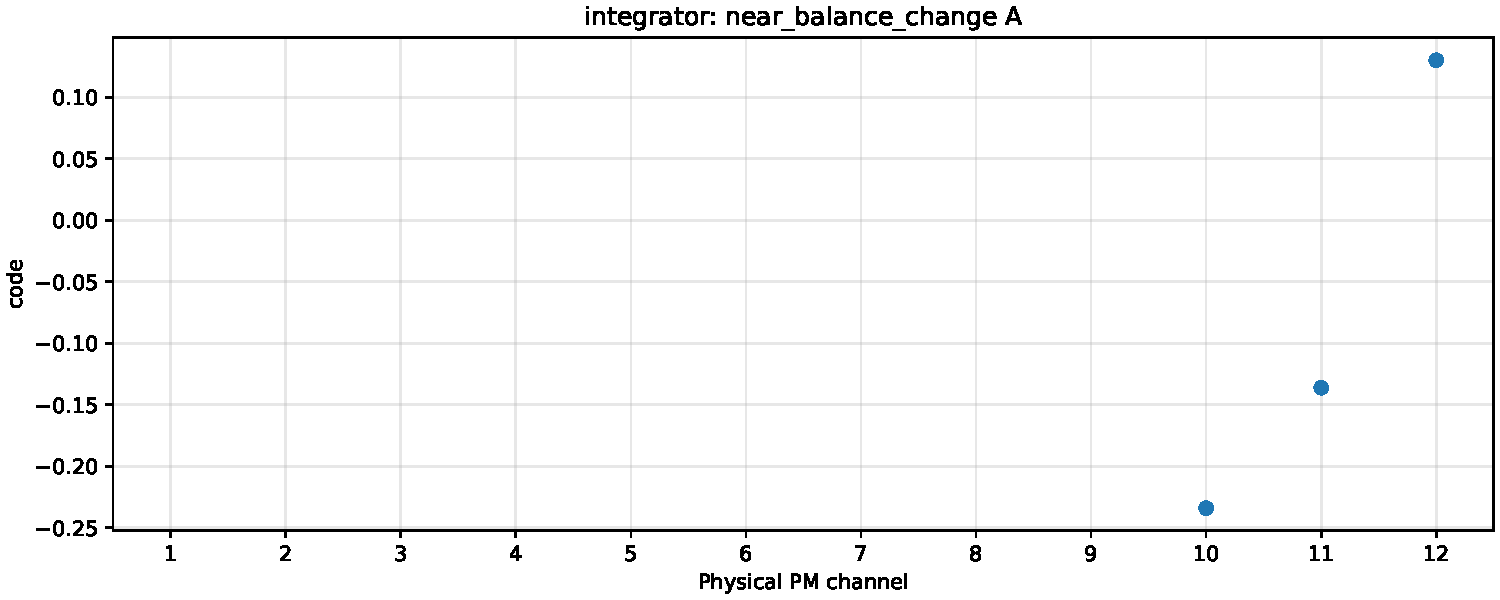
\includegraphics[width=\textwidth]{figures/figure-029.pdf}\end{center}
\begin{center}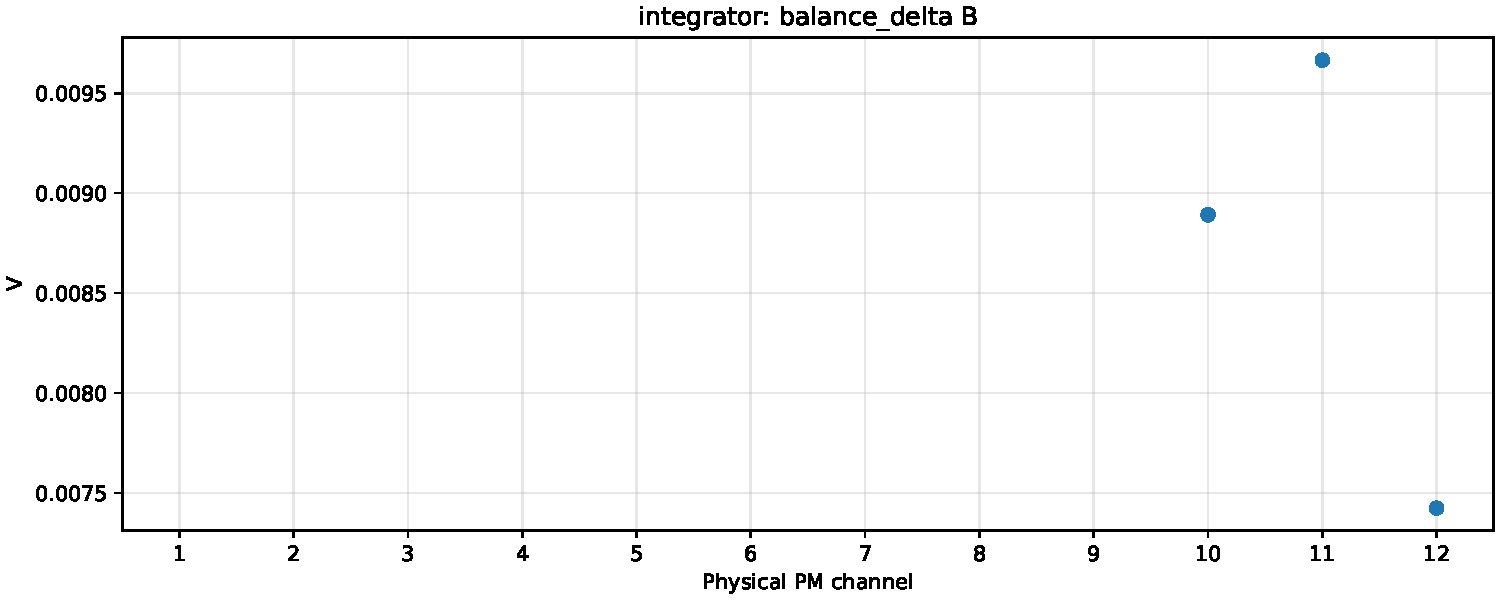
\includegraphics[width=\textwidth]{figures/figure-030.pdf}\end{center}
\begin{center}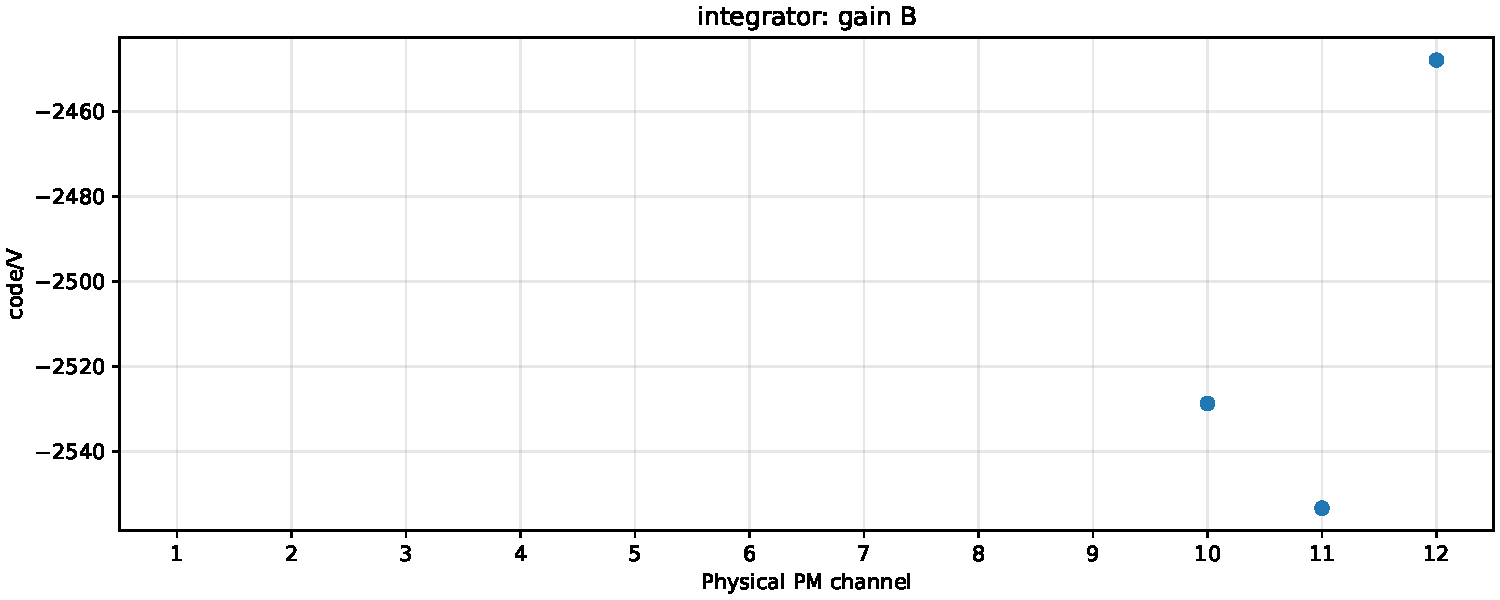
\includegraphics[width=\textwidth]{figures/figure-031.pdf}\end{center}
\begin{center}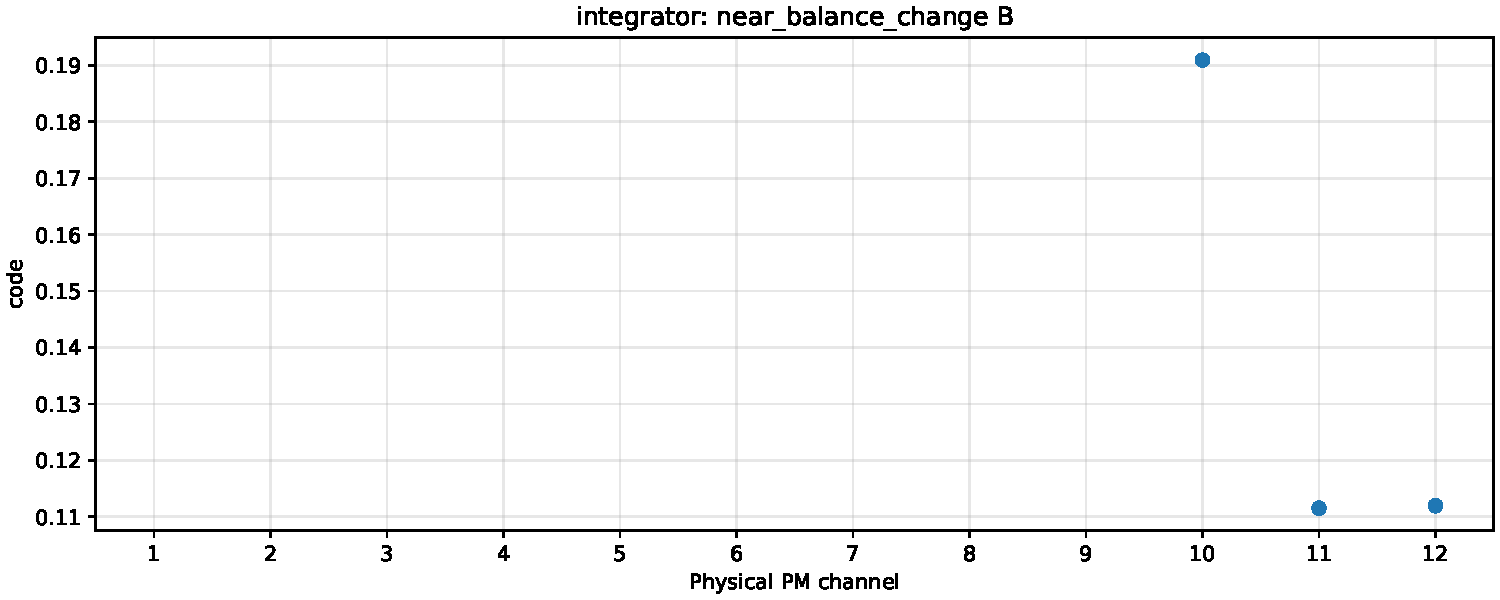
\includegraphics[width=\textwidth]{figures/figure-032.pdf}\end{center}
\begin{center}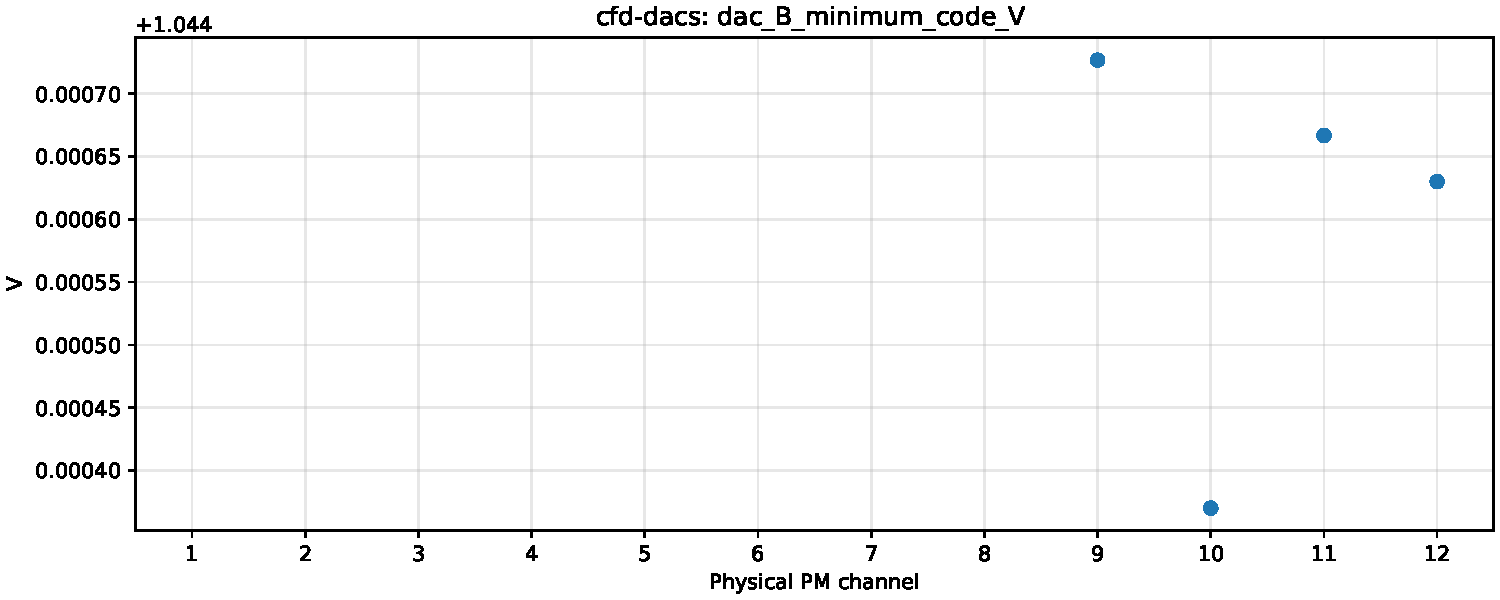
\includegraphics[width=\textwidth]{figures/figure-033.pdf}\end{center}
\begin{center}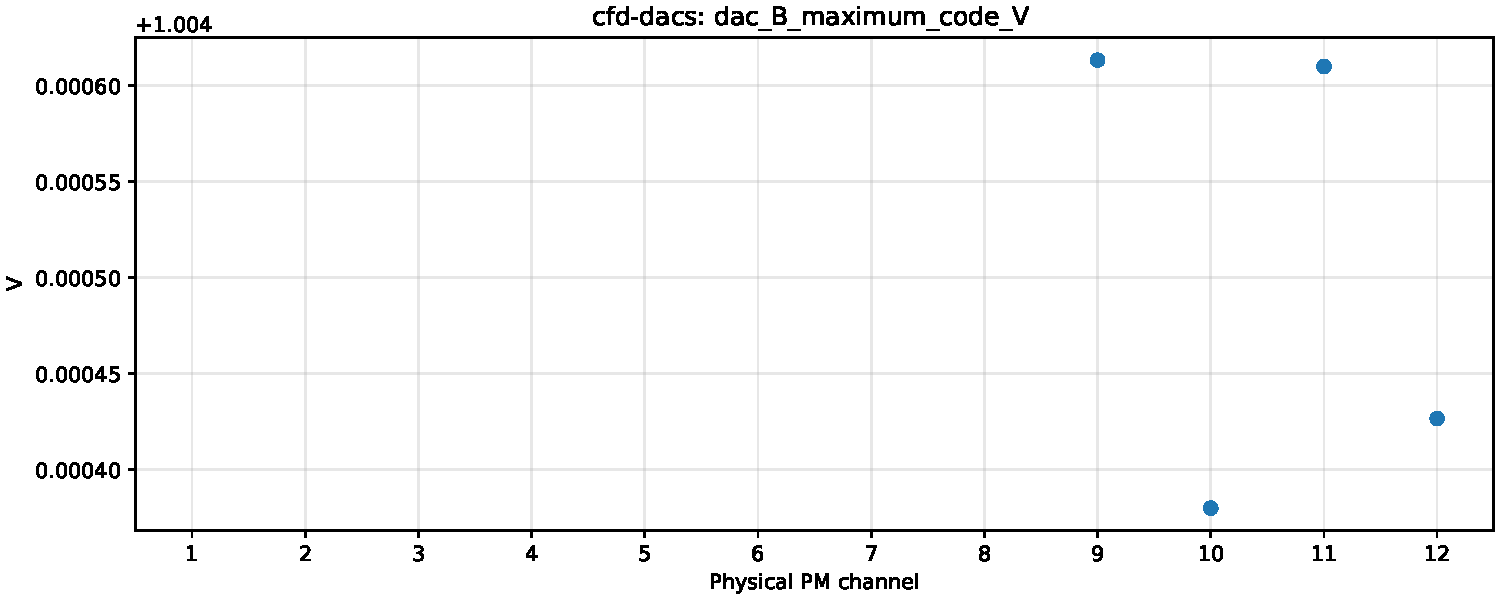
\includegraphics[width=\textwidth]{figures/figure-034.pdf}\end{center}
\begin{center}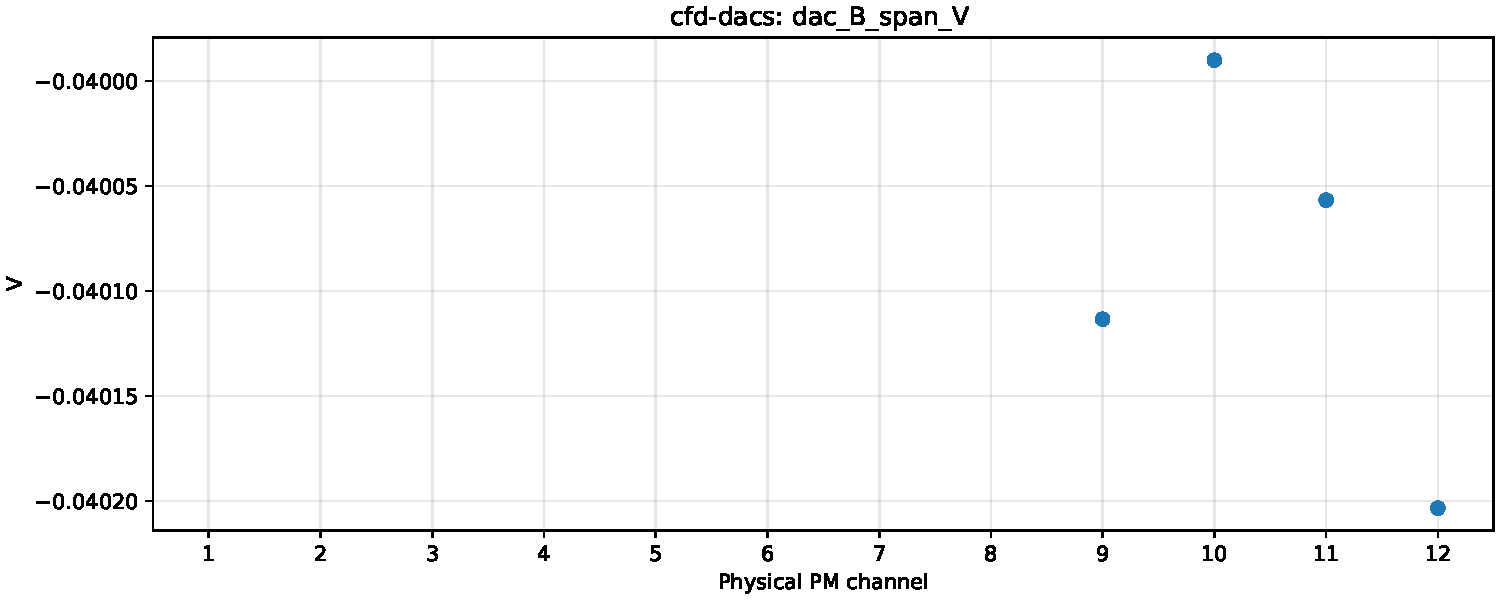
\includegraphics[width=\textwidth]{figures/figure-035.pdf}\end{center}
\begin{center}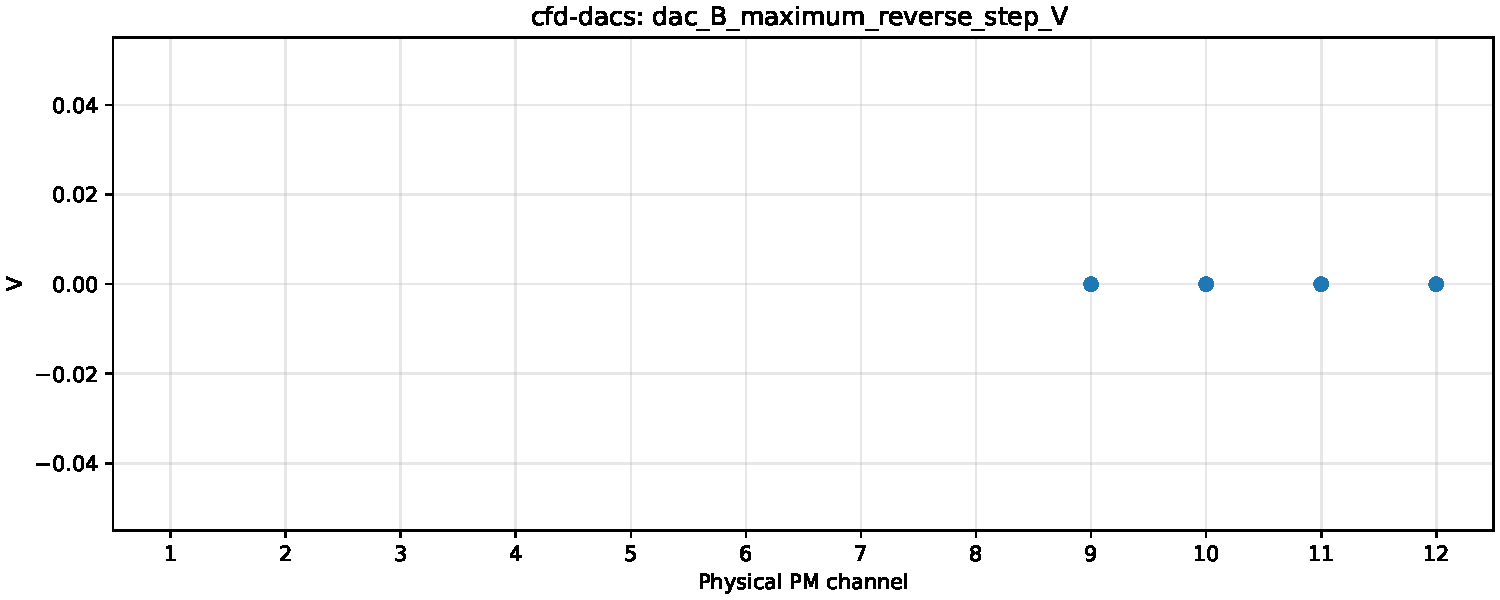
\includegraphics[width=\textwidth]{figures/figure-036.pdf}\end{center}
\begin{center}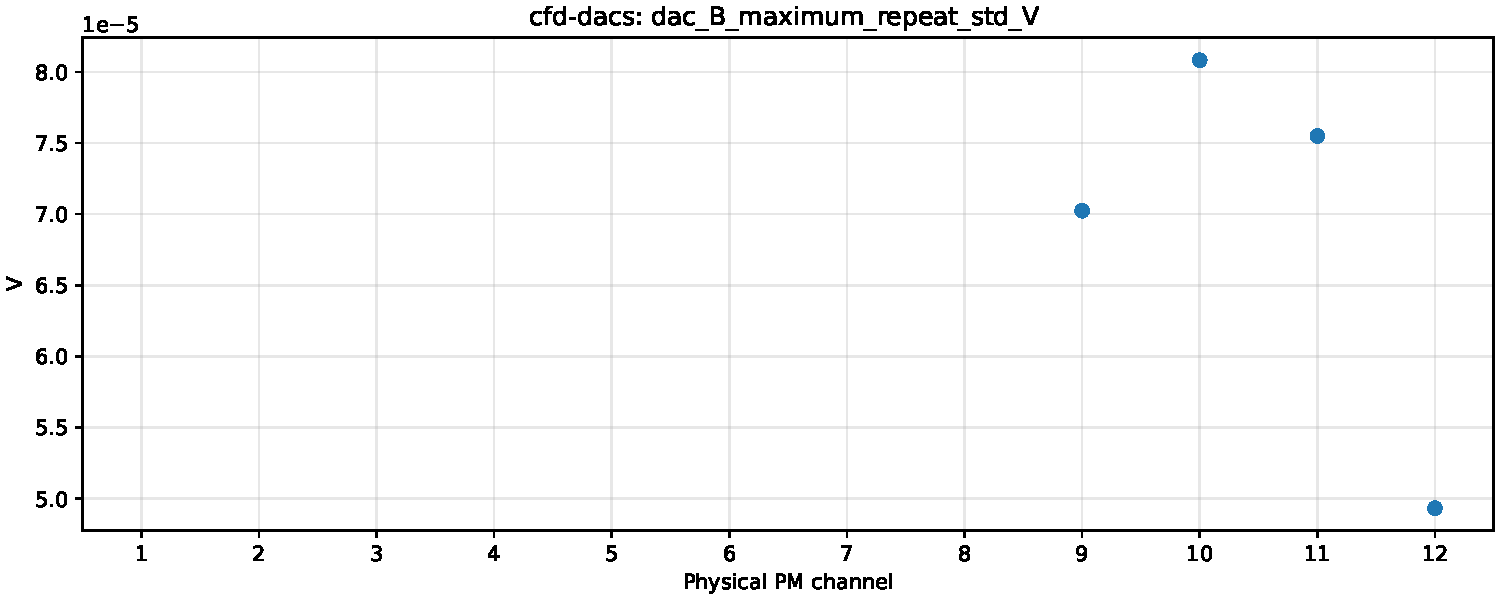
\includegraphics[width=\textwidth]{figures/figure-037.pdf}\end{center}
\begin{center}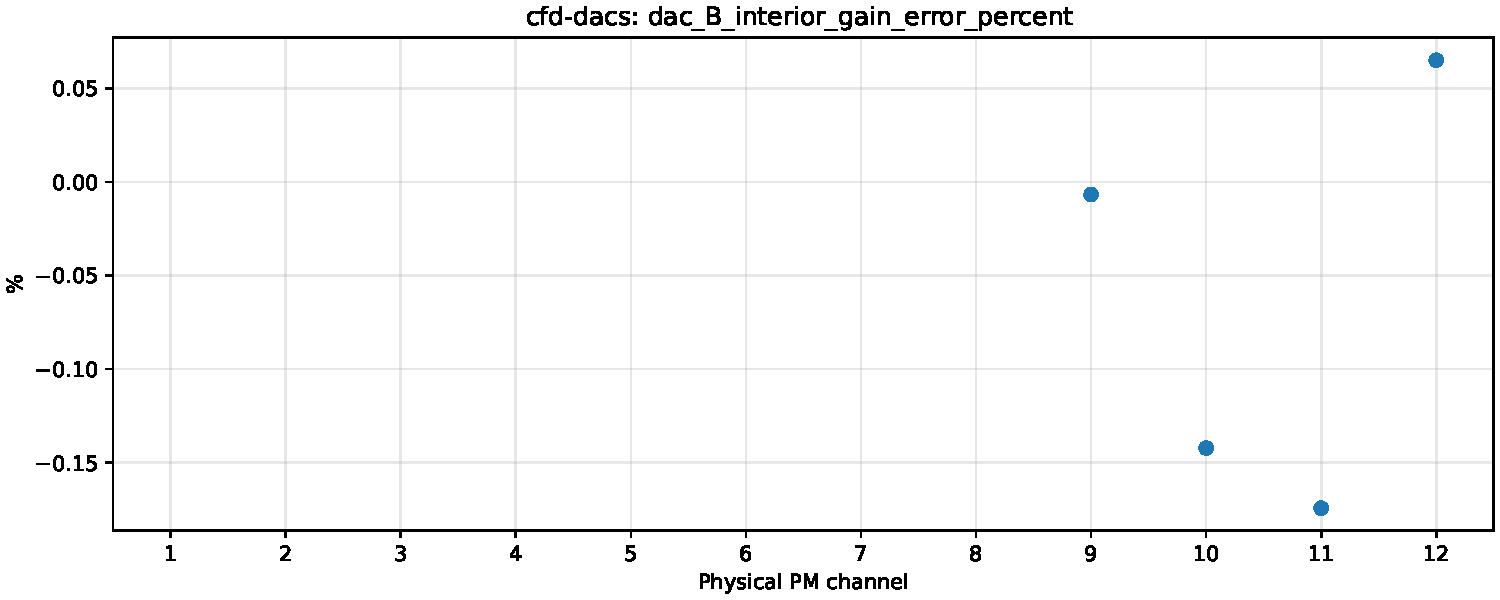
\includegraphics[width=\textwidth]{figures/figure-038.pdf}\end{center}
\begin{center}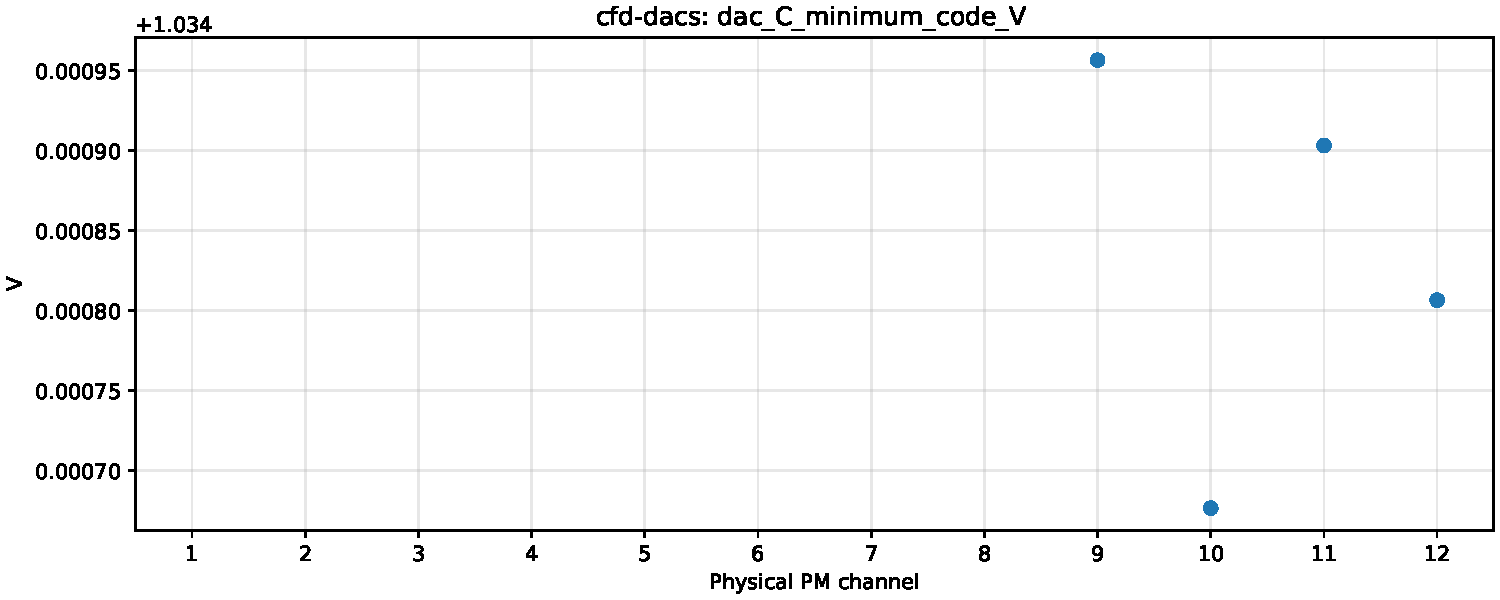
\includegraphics[width=\textwidth]{figures/figure-039.pdf}\end{center}
\begin{center}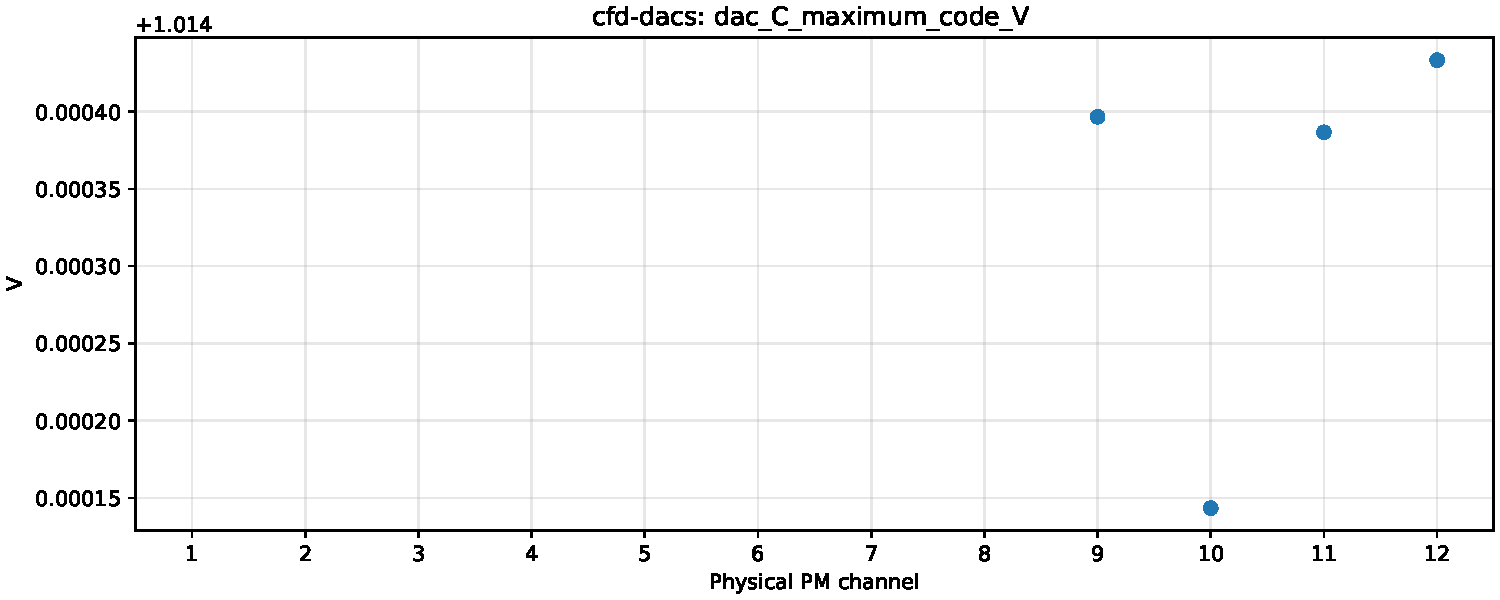
\includegraphics[width=\textwidth]{figures/figure-040.pdf}\end{center}
\begin{center}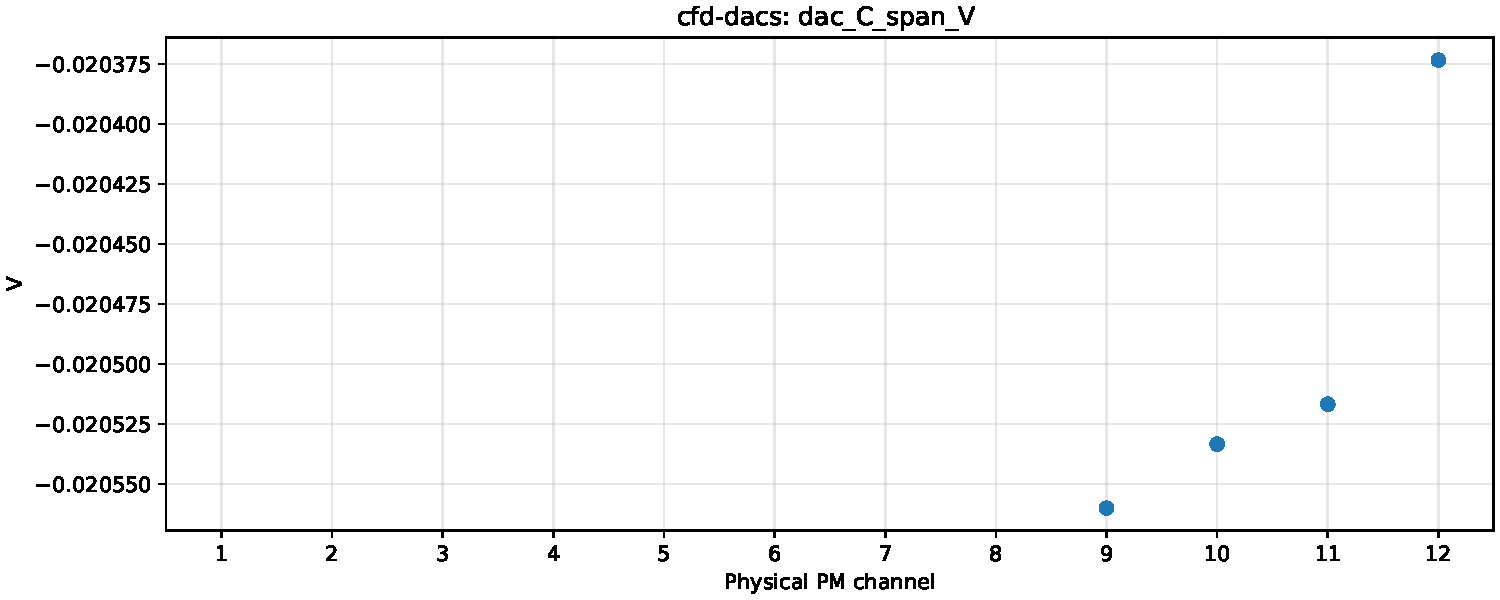
\includegraphics[width=\textwidth]{figures/figure-041.pdf}\end{center}
\begin{center}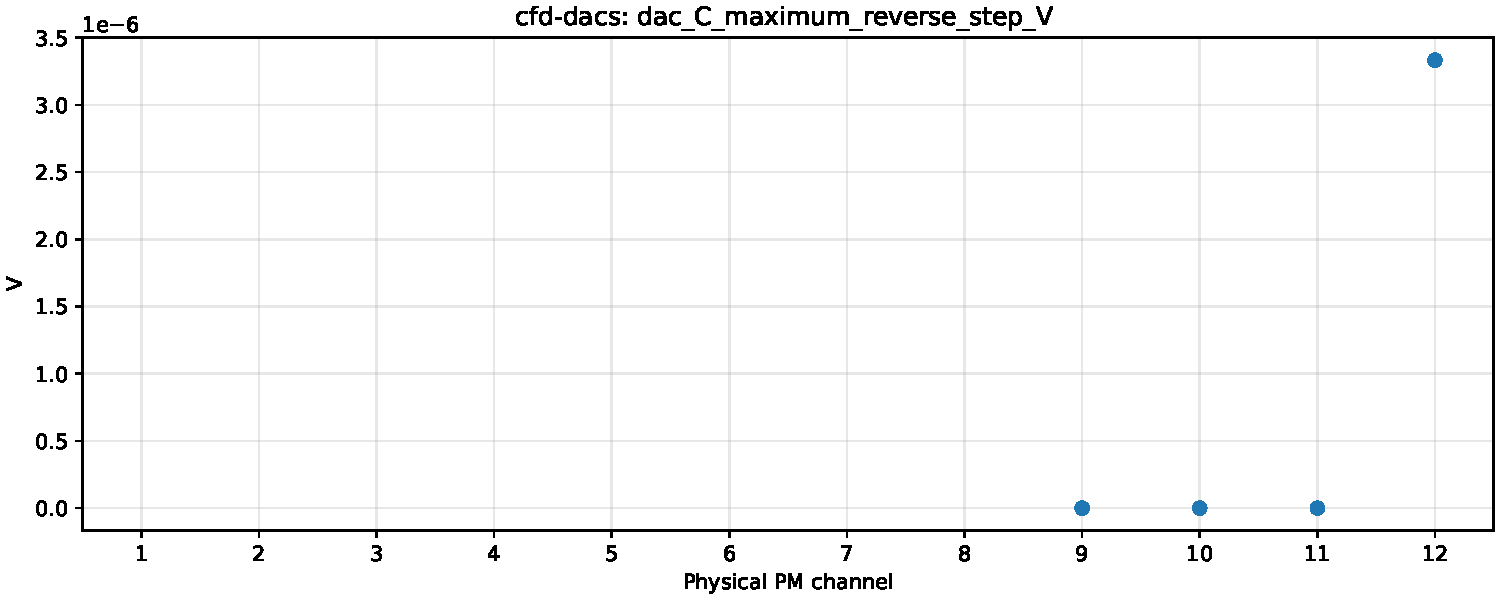
\includegraphics[width=\textwidth]{figures/figure-042.pdf}\end{center}
\begin{center}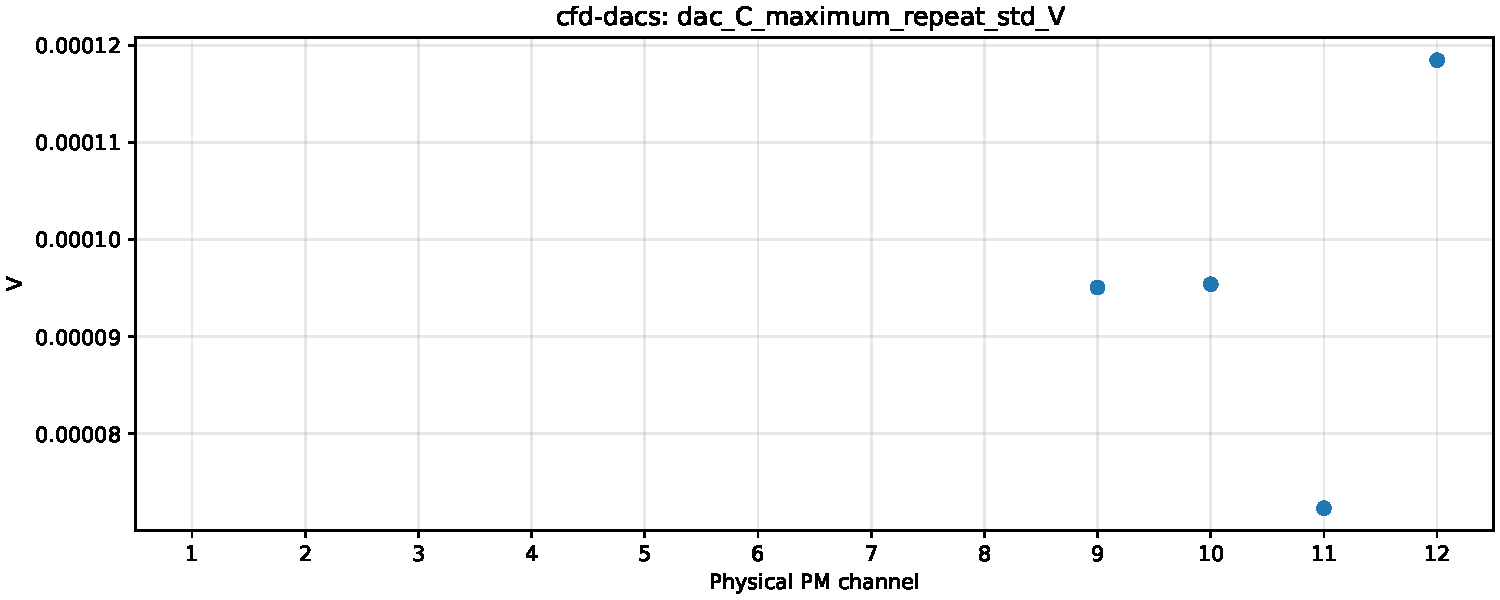
\includegraphics[width=\textwidth]{figures/figure-043.pdf}\end{center}
\begin{center}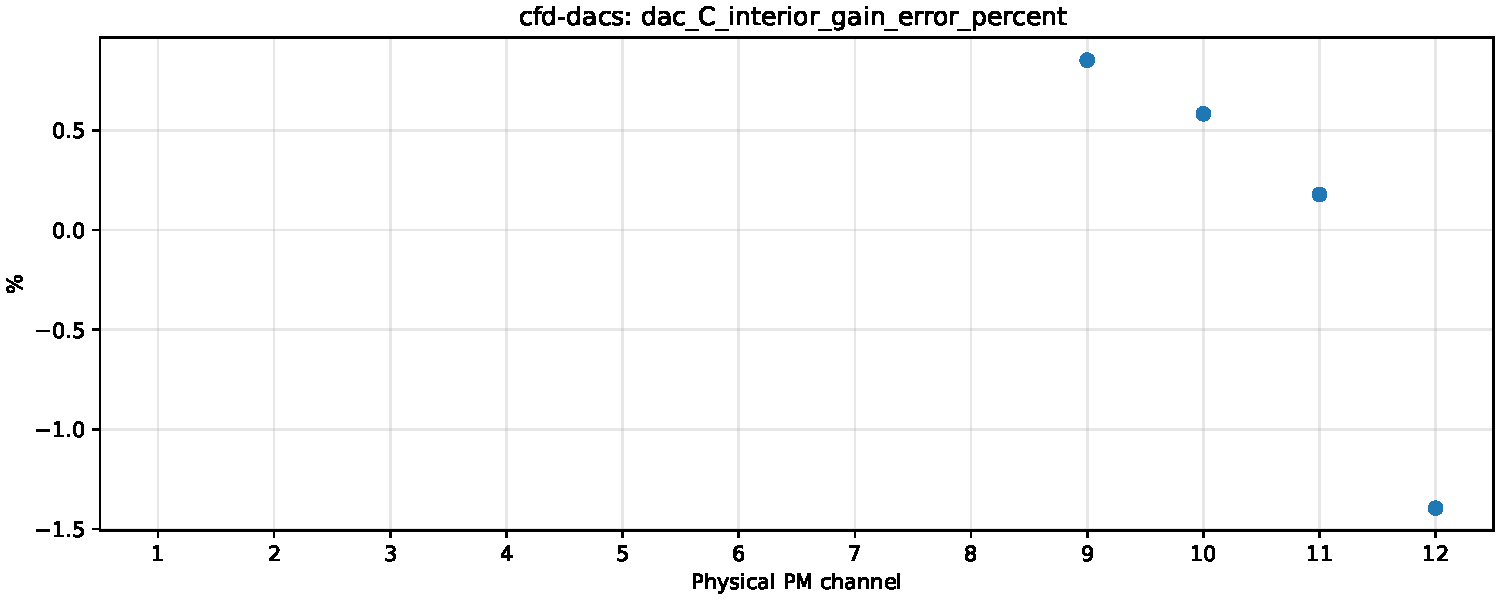
\includegraphics[width=\textwidth]{figures/figure-044.pdf}\end{center}
\begin{center}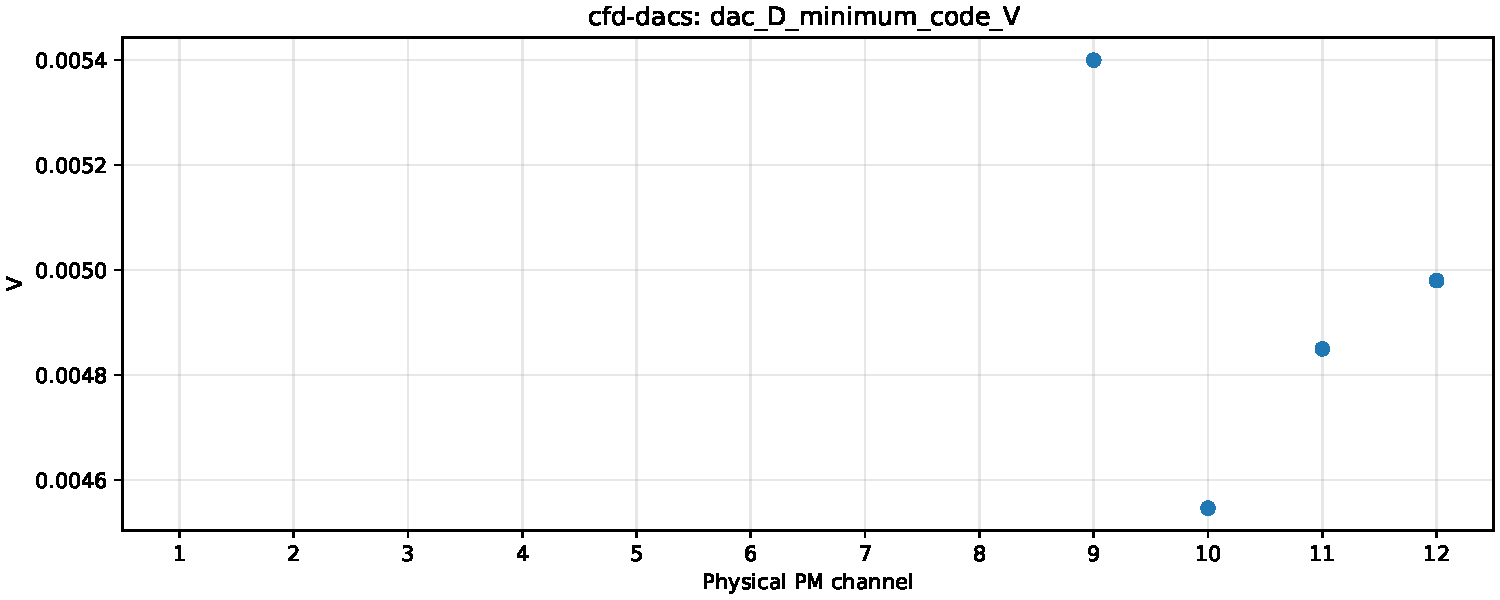
\includegraphics[width=\textwidth]{figures/figure-045.pdf}\end{center}
\begin{center}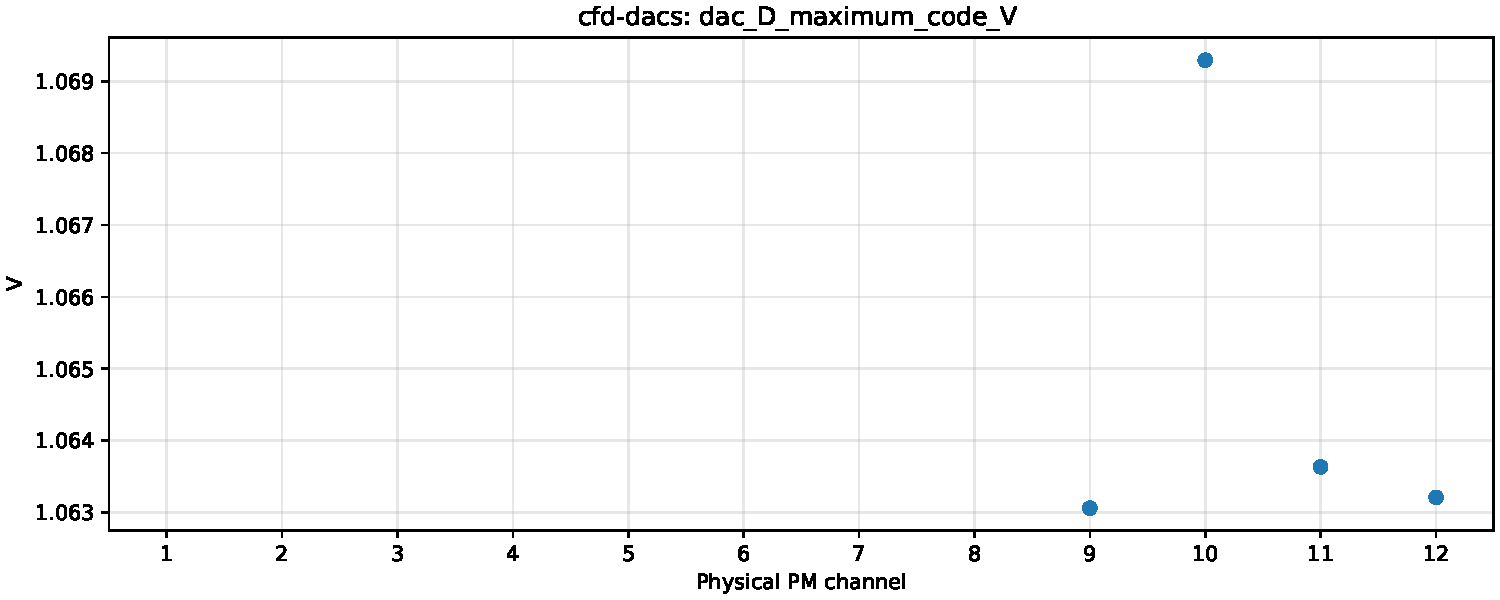
\includegraphics[width=\textwidth]{figures/figure-046.pdf}\end{center}
\begin{center}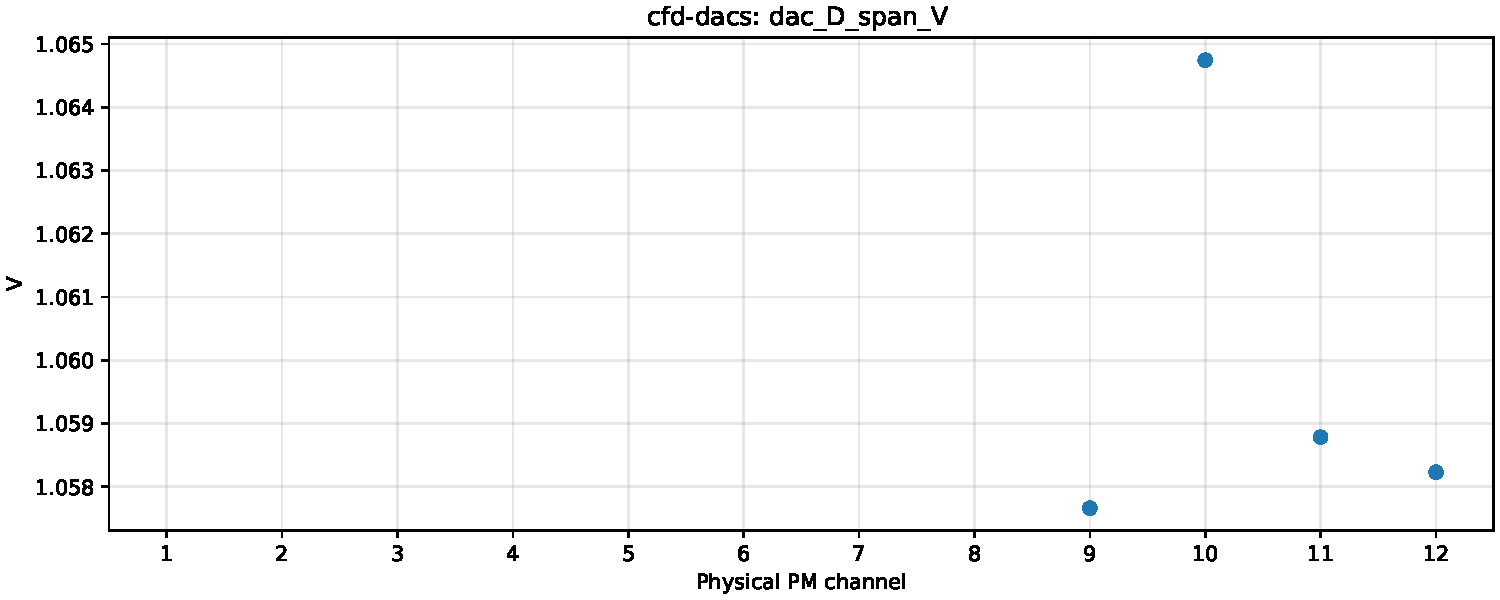
\includegraphics[width=\textwidth]{figures/figure-047.pdf}\end{center}
\begin{center}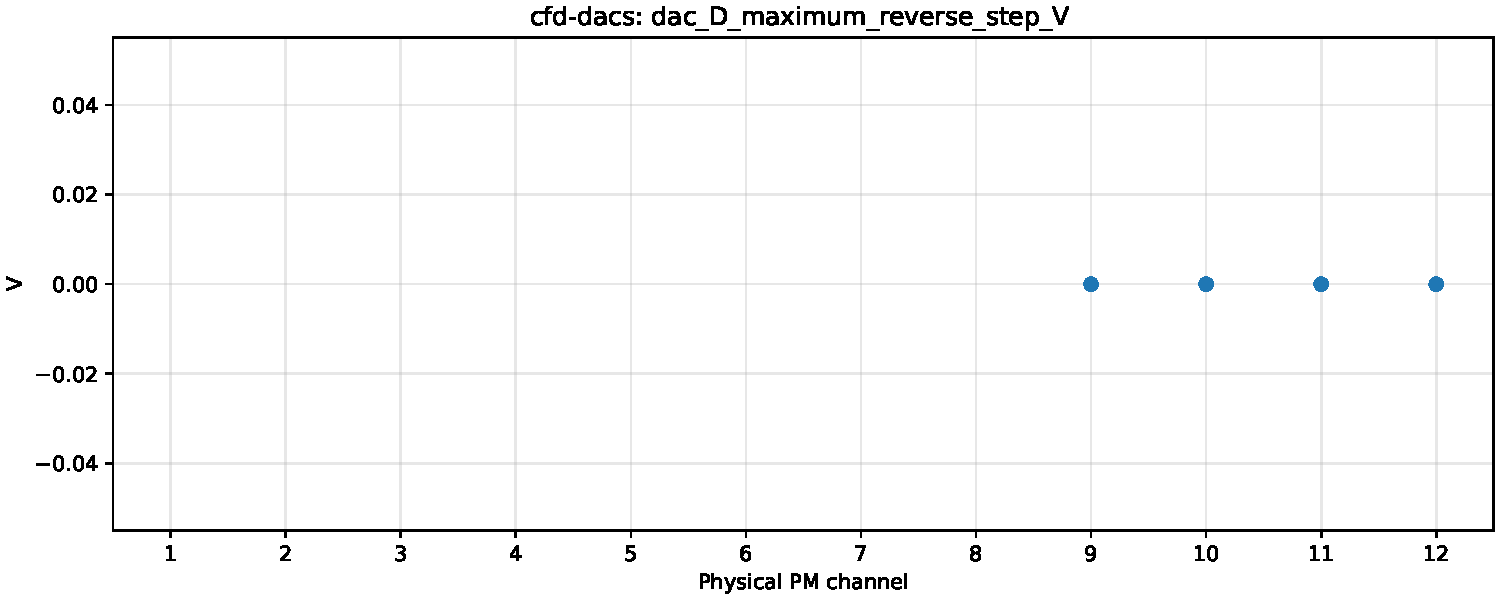
\includegraphics[width=\textwidth]{figures/figure-048.pdf}\end{center}
\begin{center}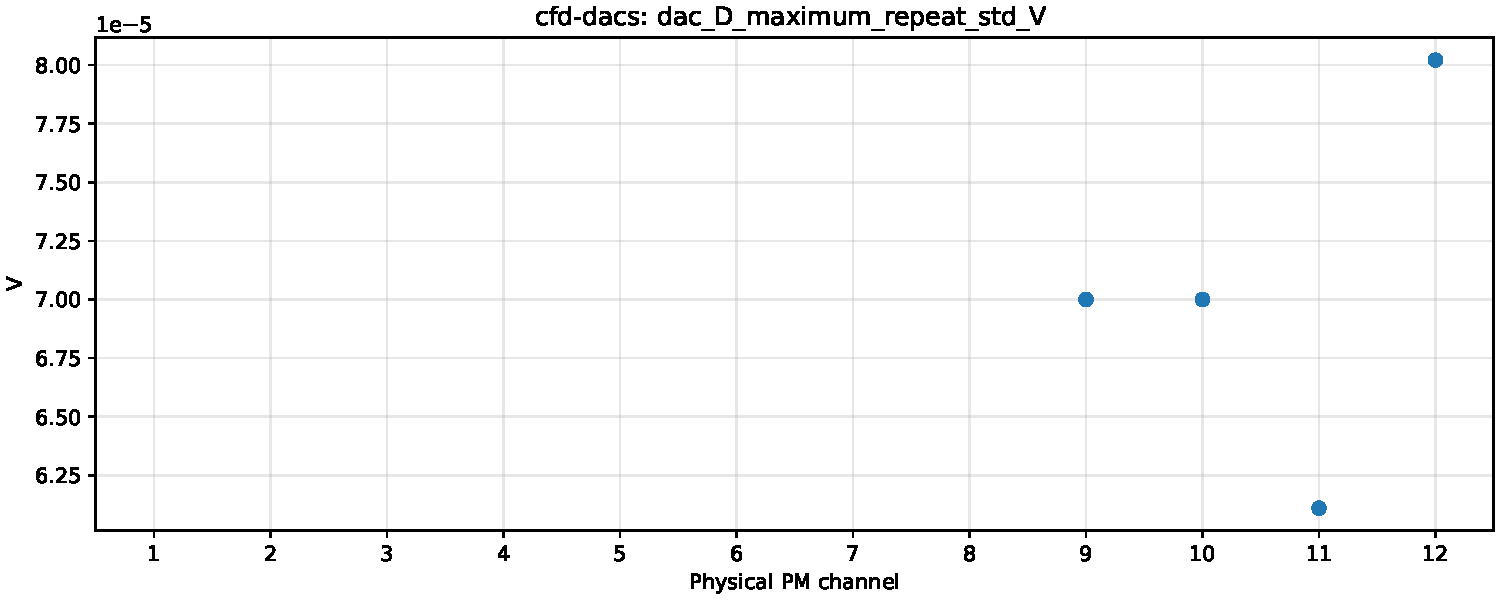
\includegraphics[width=\textwidth]{figures/figure-049.pdf}\end{center}
\begin{center}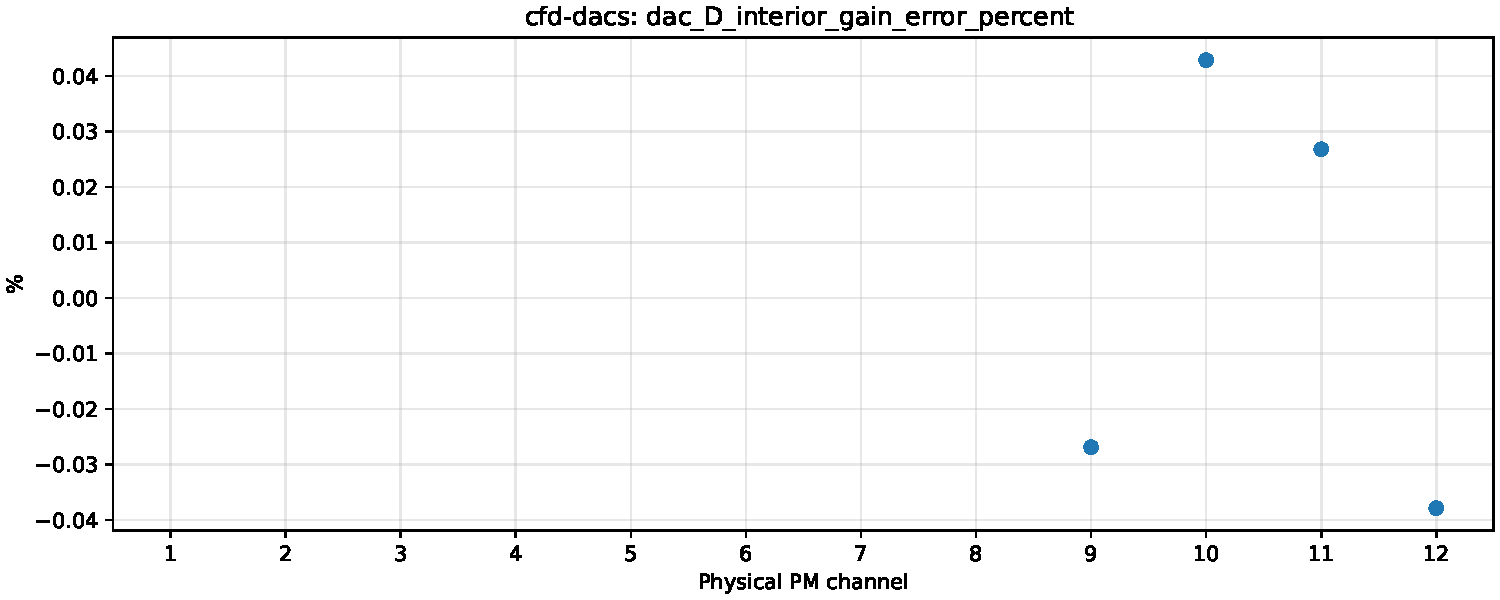
\includegraphics[width=\textwidth]{figures/figure-050.pdf}\end{center}
\begin{center}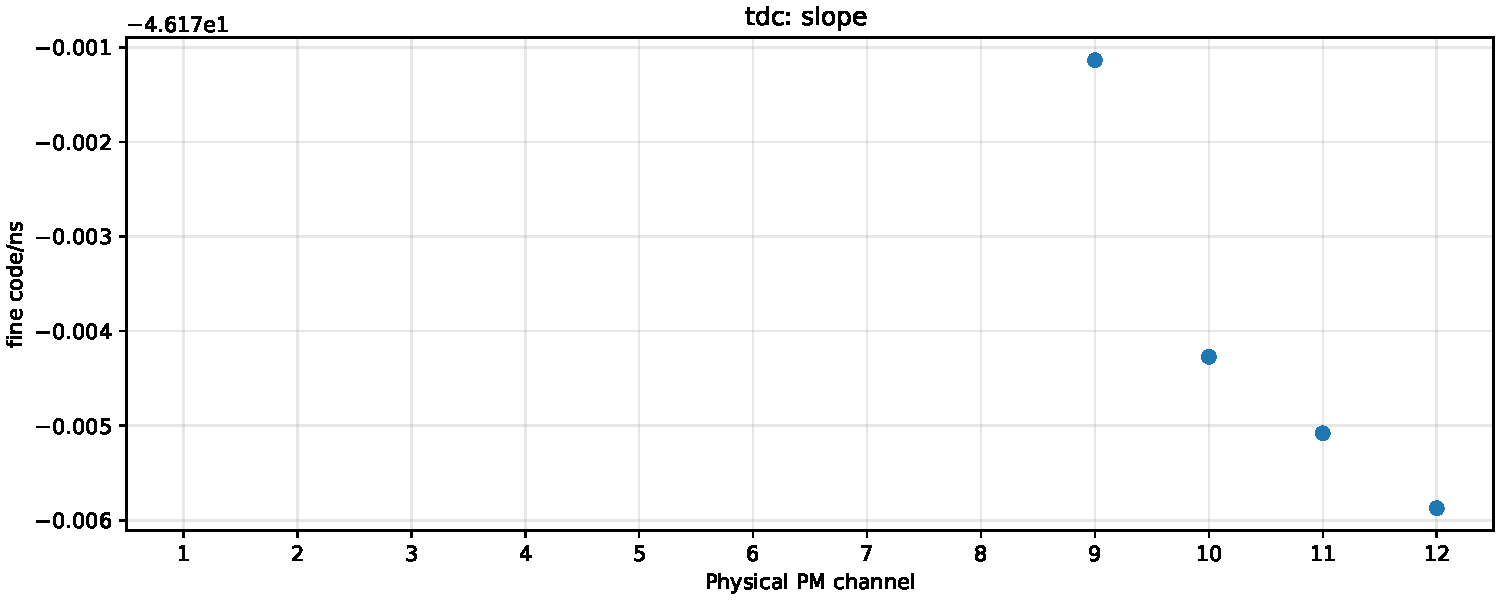
\includegraphics[width=\textwidth]{figures/figure-051.pdf}\end{center}
\begin{center}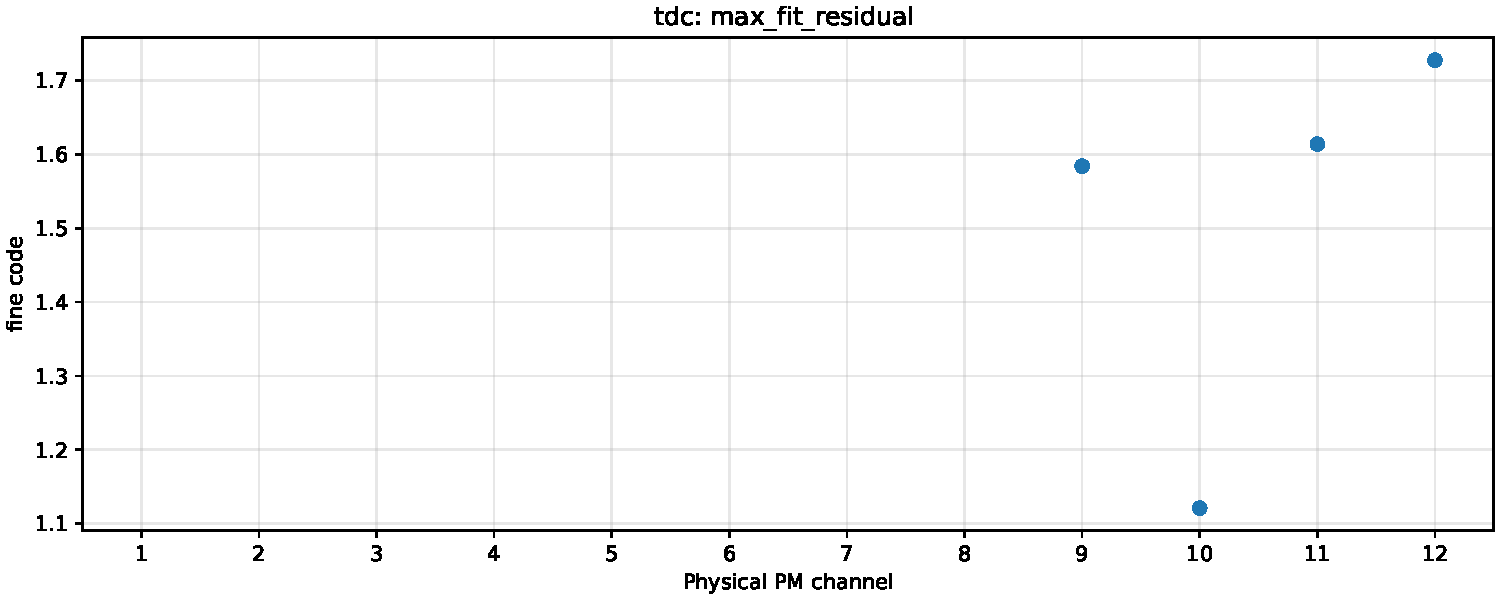
\includegraphics[width=\textwidth]{figures/figure-052.pdf}\end{center}
\begin{center}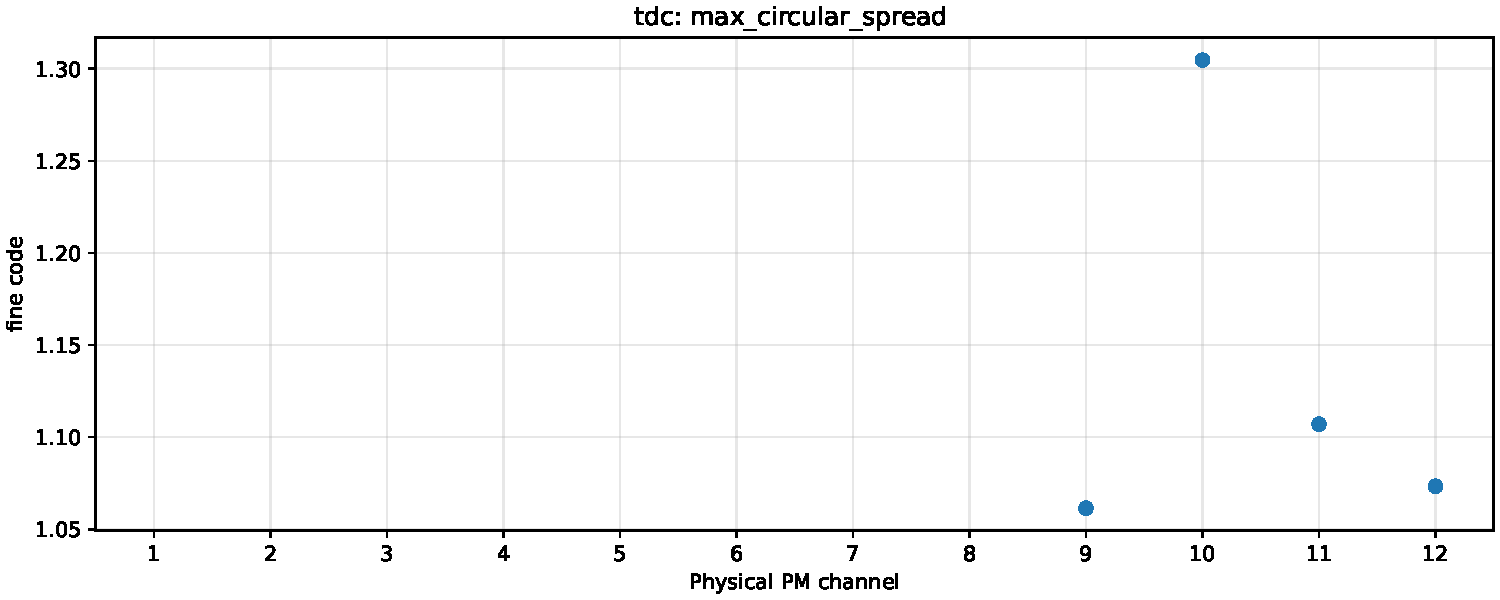
\includegraphics[width=\textwidth]{figures/figure-053.pdf}\end{center}
\begin{center}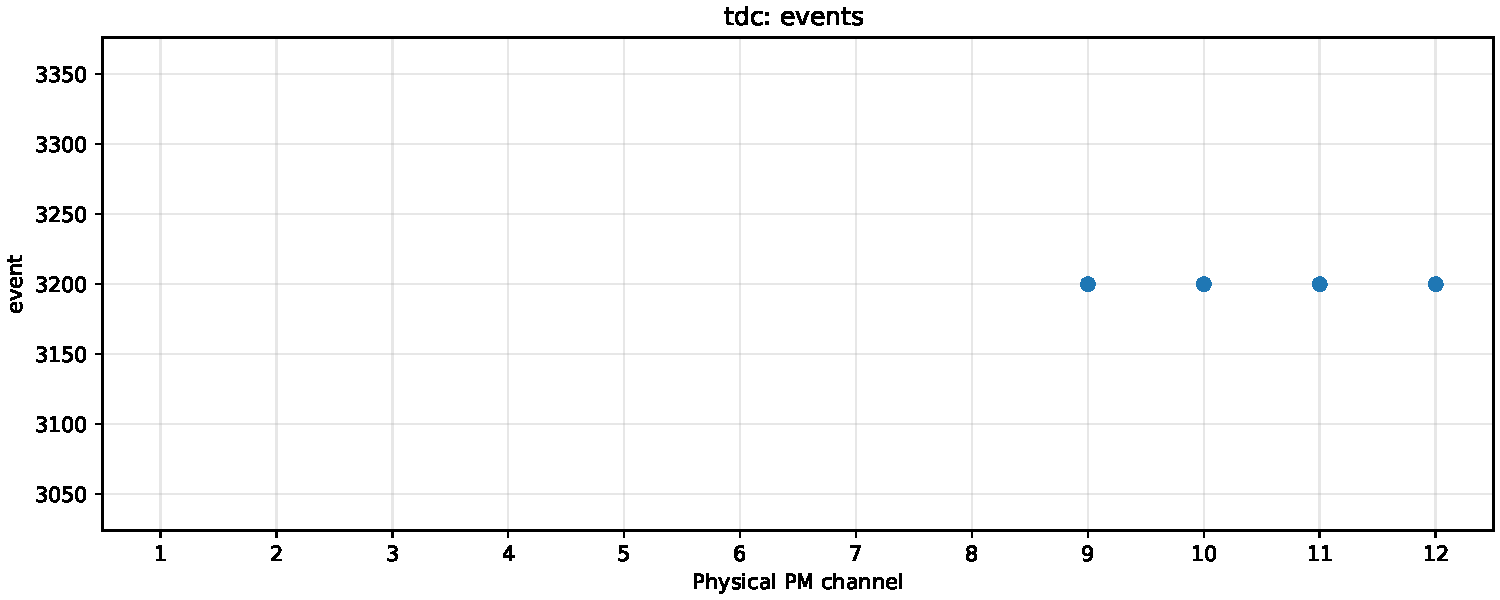
\includegraphics[width=\textwidth]{figures/figure-054.pdf}\end{center}
\begin{center}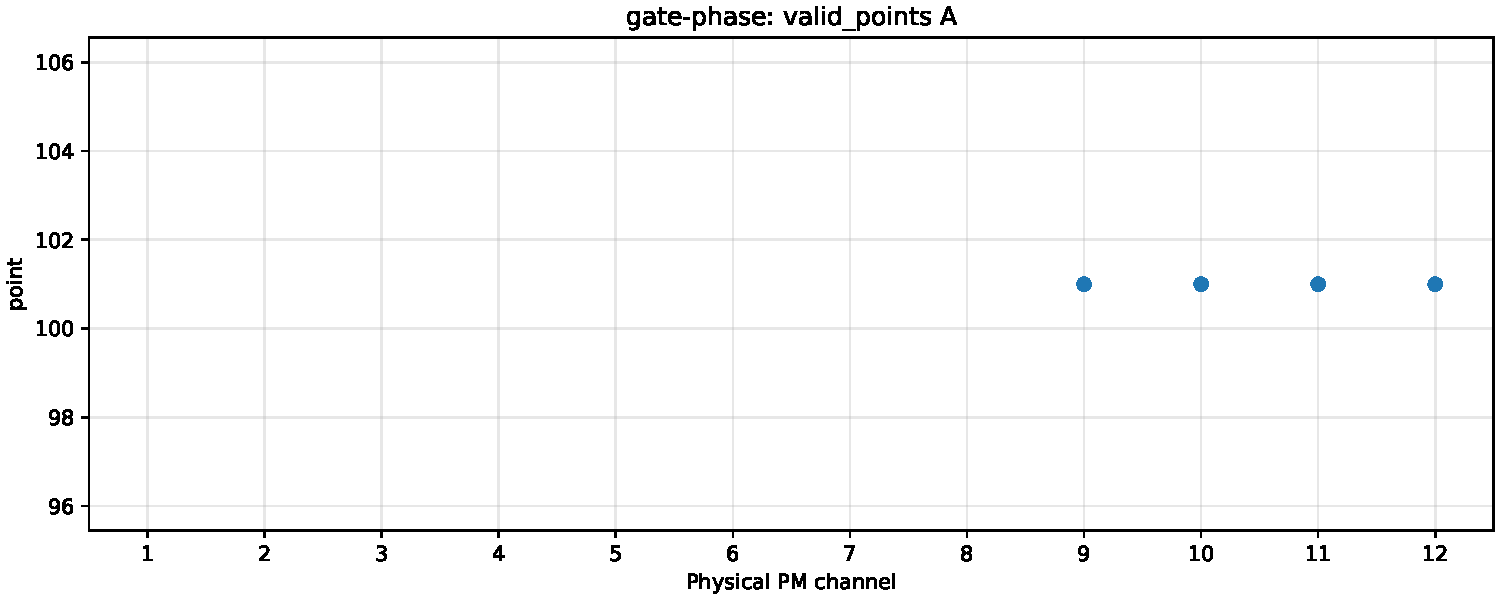
\includegraphics[width=\textwidth]{figures/figure-055.pdf}\end{center}
\begin{center}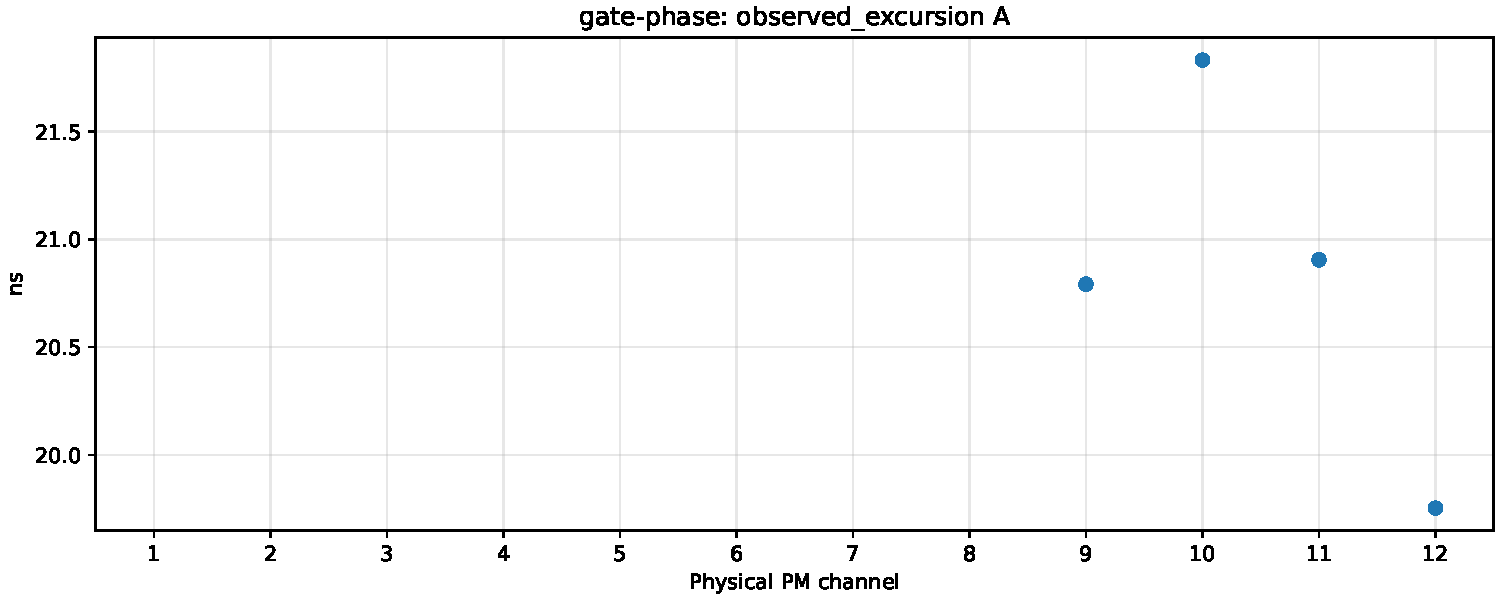
\includegraphics[width=\textwidth]{figures/figure-056.pdf}\end{center}
\begin{center}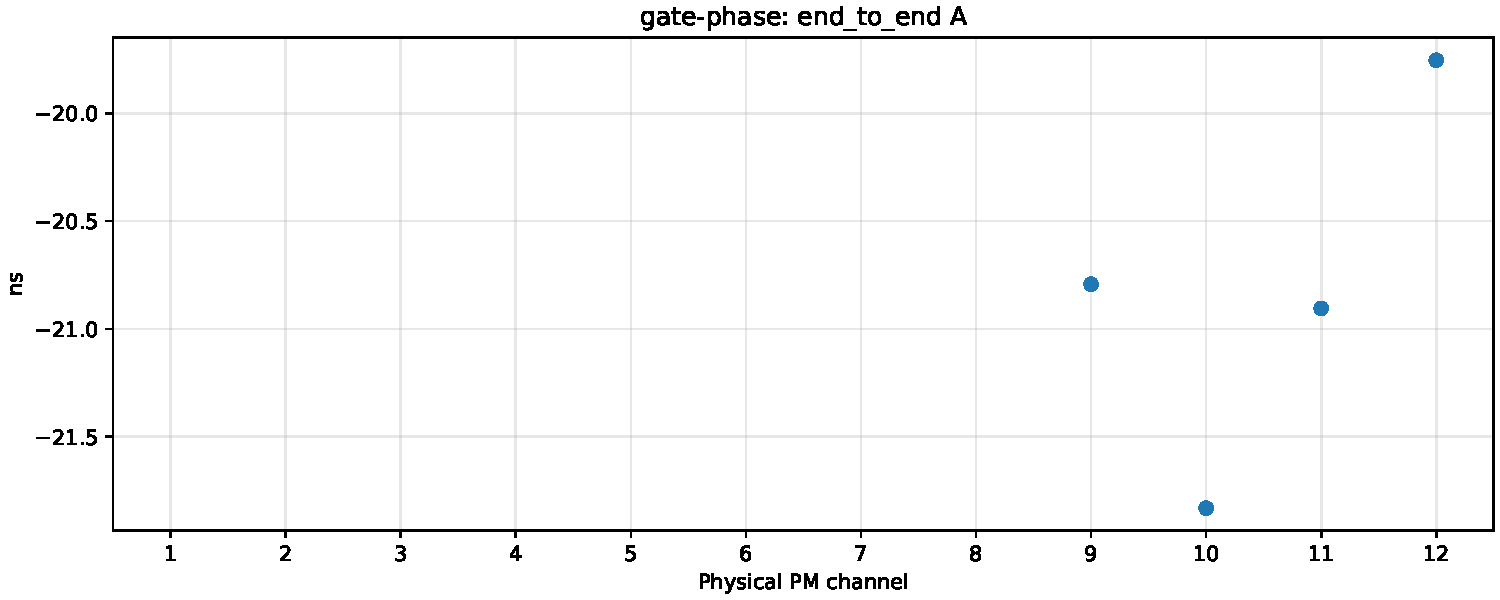
\includegraphics[width=\textwidth]{figures/figure-057.pdf}\end{center}
\begin{center}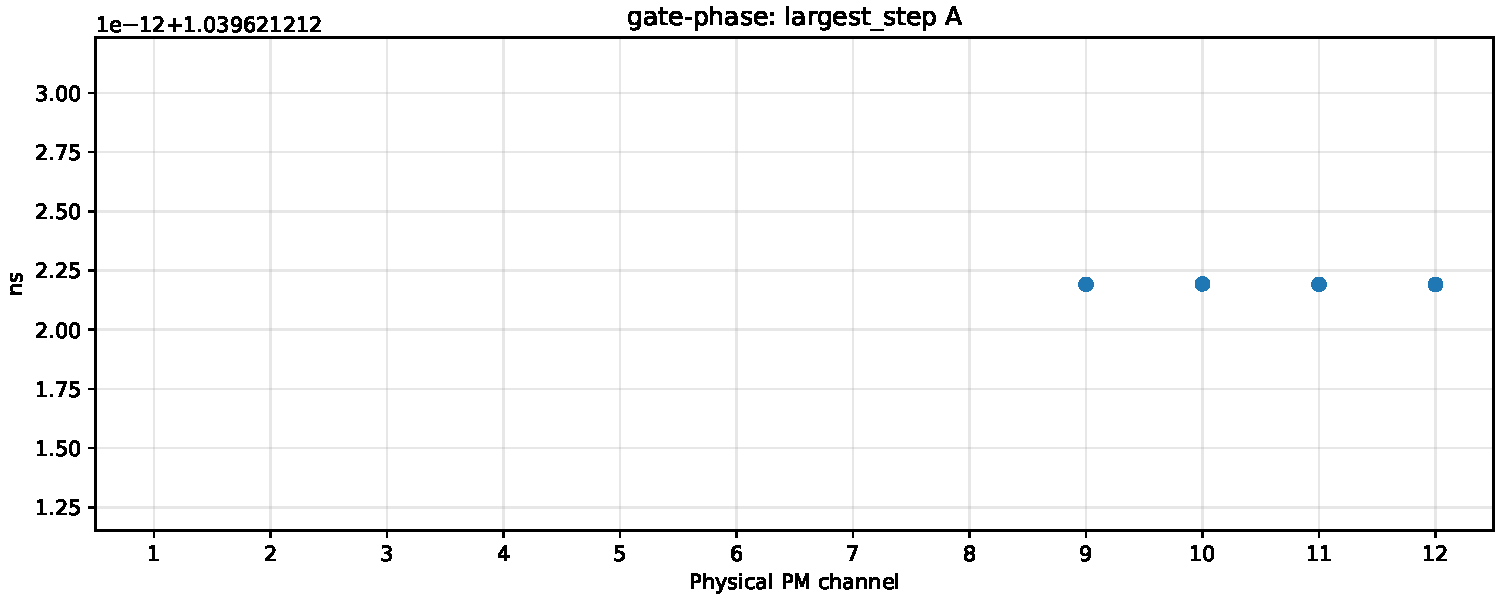
\includegraphics[width=\textwidth]{figures/figure-058.pdf}\end{center}
\begin{center}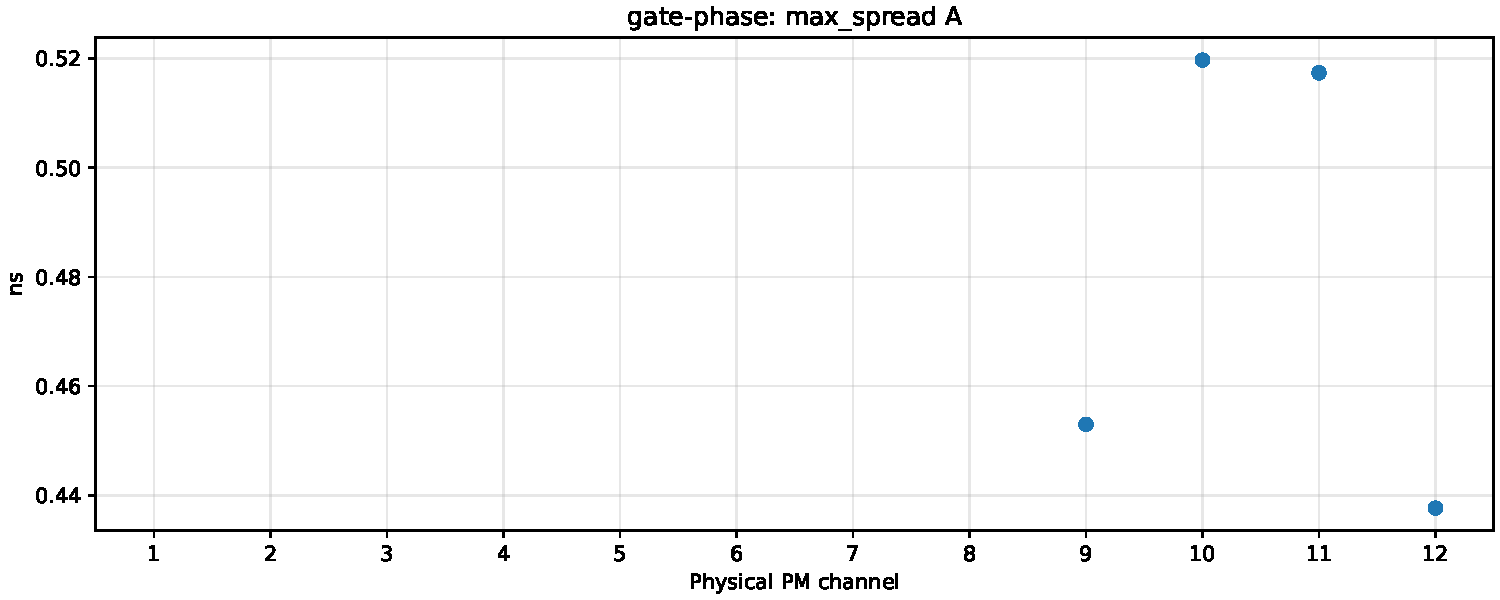
\includegraphics[width=\textwidth]{figures/figure-059.pdf}\end{center}
\begin{center}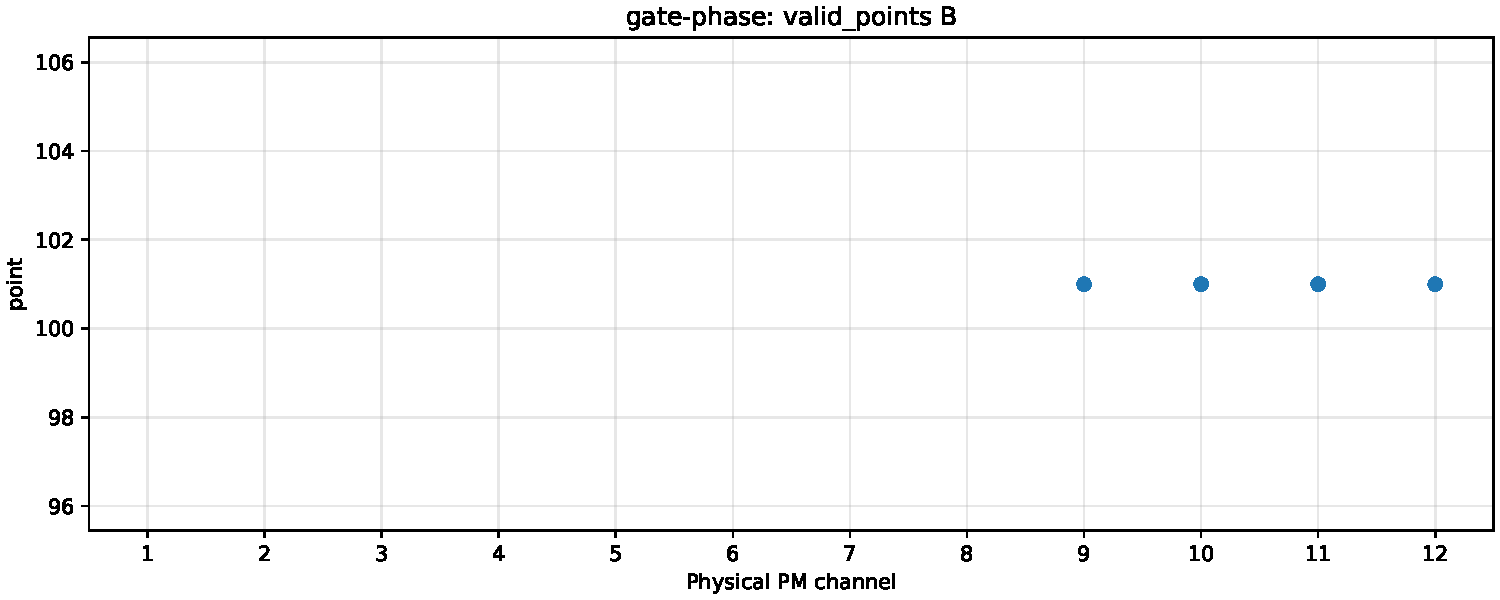
\includegraphics[width=\textwidth]{figures/figure-060.pdf}\end{center}
\begin{center}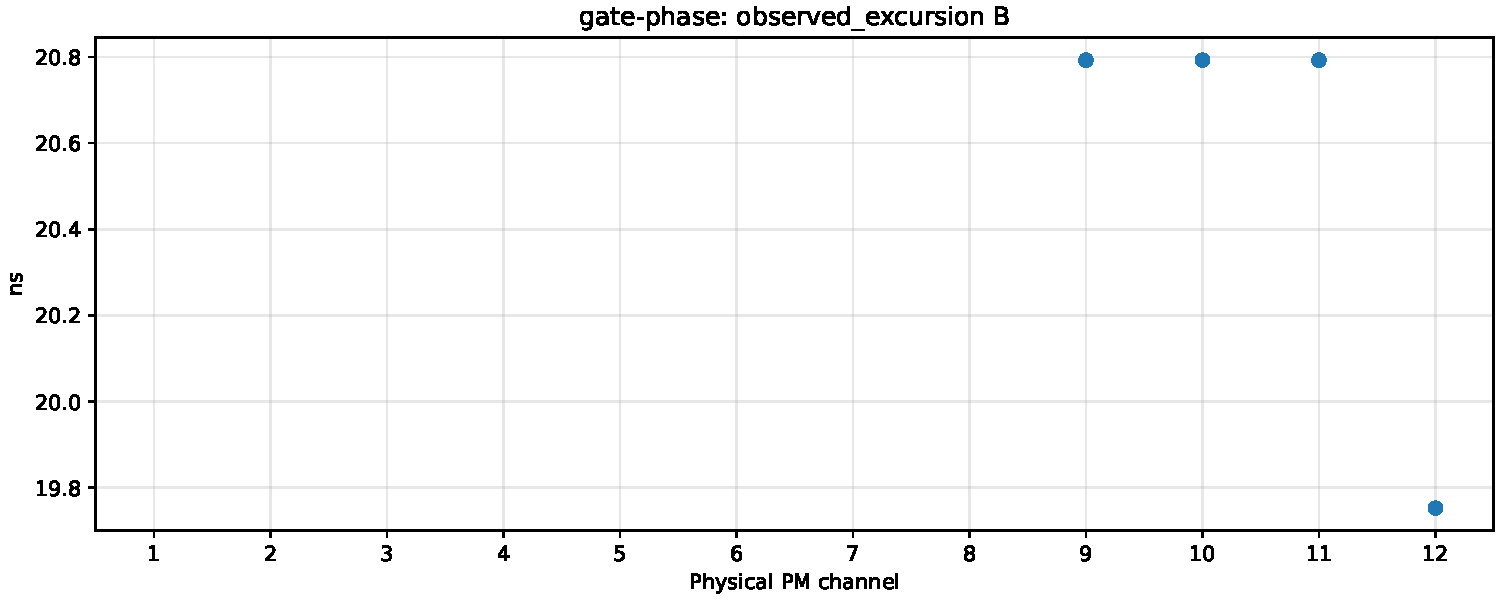
\includegraphics[width=\textwidth]{figures/figure-061.pdf}\end{center}
\begin{center}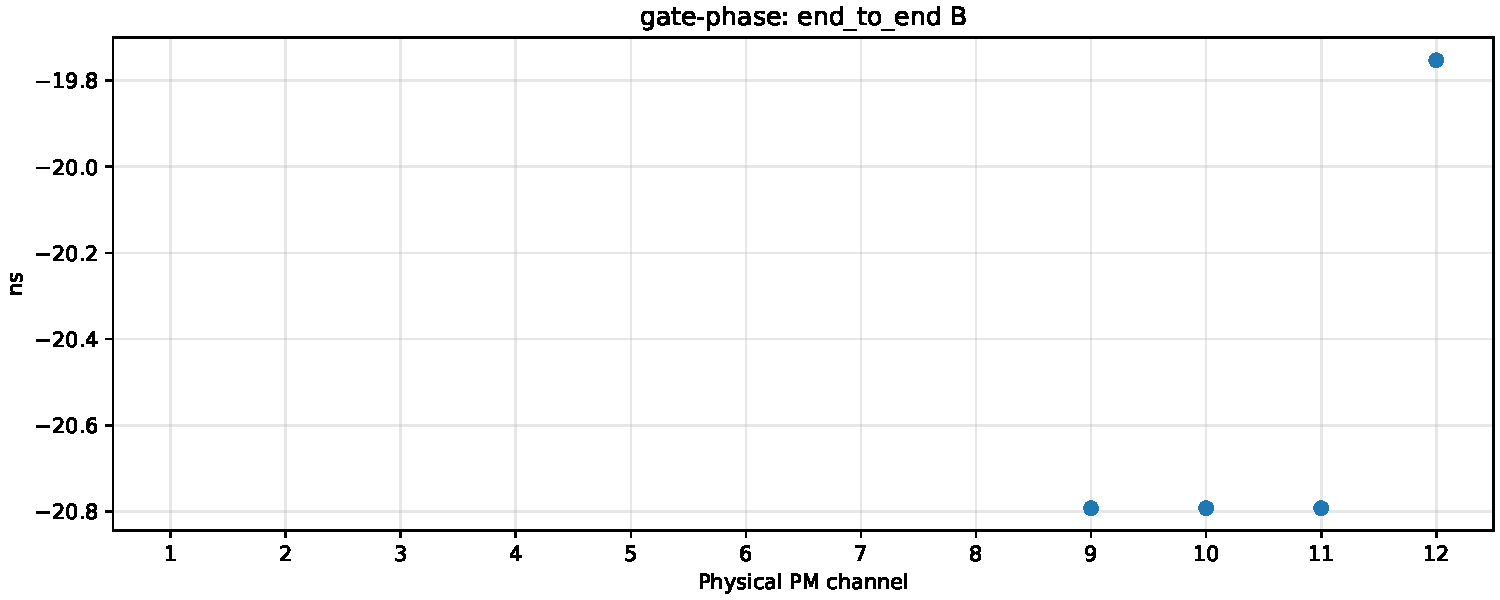
\includegraphics[width=\textwidth]{figures/figure-062.pdf}\end{center}
\begin{center}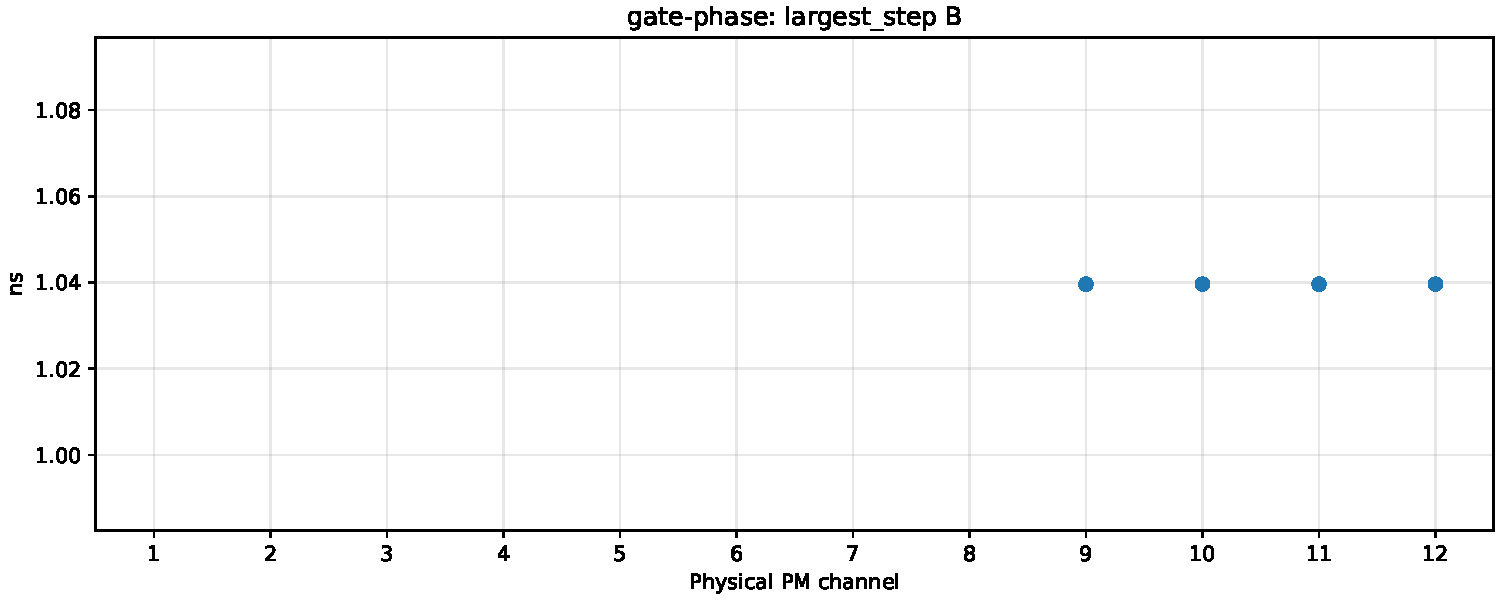
\includegraphics[width=\textwidth]{figures/figure-063.pdf}\end{center}
\begin{center}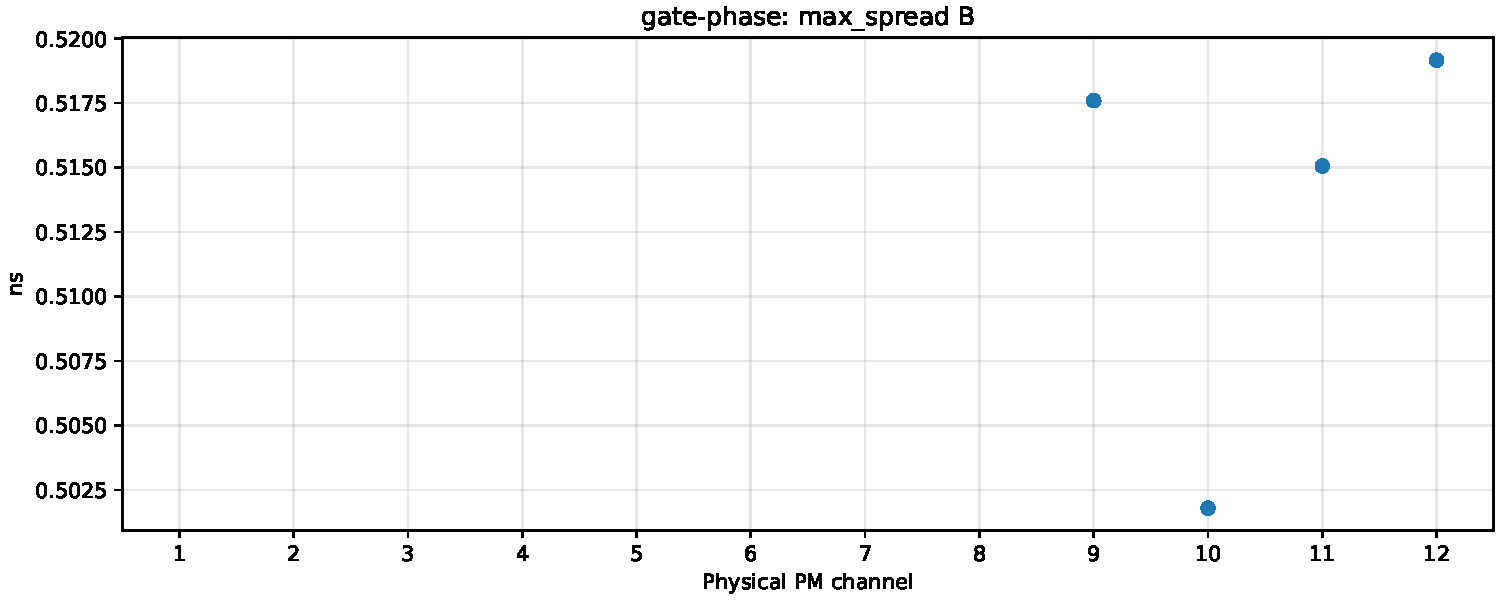
\includegraphics[width=\textwidth]{figures/figure-064.pdf}\end{center}
